\part{RL Methods for LLMs}

\chapter{RL Foundations for Language Models}
\label{rl-foundations-for-language-models}

Supervised fine-tuning (SFT) teaches a model to imitate demonstrations, but imitation has a ceiling: the model can never exceed the quality of its training data. Reinforcement learning breaks this barrier. By generating novel text, receiving reward feedback, and updating toward higher-reward behaviours, an RL-trained model can \emph{discover} strategies that no human demonstrator wrote---producing outputs that are more helpful, more accurate, and better aligned with human preferences~\cite{ouyang2022training}.

This is the mechanism behind every frontier model: GPT-4~\cite{openai2023gpt4}, Claude, Llama-3~\cite{grattafiori2024llama3}, and DeepSeek-R1~\cite{deepseek2025r1} all apply RL after SFT as the critical step that transforms a capable but unsteered model into an aligned assistant.

\section{Two Paradigms for RL in LLMs}
\label{two-paradigms-rl-llms}

RL methods for language models fall into two broad paradigms, each suited to different goals:

\paragraph{Paradigm 1: Alignment via Human Preferences (RLHF/DPO).}
The original motivation for applying RL to LLMs was \textbf{alignment}---making models helpful, harmless, and honest. \textbf{Reinforcement Learning from Human Feedback (RLHF)}~\cite{ouyang2022training, ziegler2019fine, christiano2017deep} trains a reward model from pairwise human judgments (``which response is better?'') and then optimizes the policy to maximize that learned reward. \textbf{DPO}~\cite{rafailov2023direct} simplifies this by eliminating the reward model entirely, converting preferences directly into a supervised loss. Both approaches produce aligned assistants that follow instructions and respect safety constraints.

\paragraph{Paradigm 2: Capability Enhancement via Verifiable Rewards (RLVR).}
More recently, RL has been used not just for alignment but for \textbf{teaching new capabilities}---particularly reasoning, mathematics, and code generation. Here the reward comes not from human preferences but from \textbf{verifiable outcomes}: did the model produce the correct answer? Did the code pass all tests? DeepSeek-R1~\cite{deepseek2025r1} demonstrated that GRPO with rule-based rewards (format correctness + answer accuracy) can train models to develop sophisticated chain-of-thought reasoning \emph{without any human preference data}. This paradigm---RL from Verifiable Rewards (RLVR)---is now the dominant approach for building reasoning models and agentic systems.

\begin{keybox}[The Shared Foundation]
Despite their different goals, both paradigms share the same core machinery:
\begin{itemize}
  \item A \textbf{policy} $\pi_\theta$ (the LLM) that generates text autoregressively
  \item A \textbf{reward signal} $r(x, y)$ (learned from preferences or computed from verification)
  \item A \textbf{KL constraint} against a reference policy to prevent degenerate solutions
  \item \textbf{Policy gradient optimization} (PPO or GRPO) to update the model toward higher reward
\end{itemize}
The chapters in this part develop each component in detail.
\end{keybox}

\section{Text Generation as an MDP}
\label{text-generation-as-mdp}

The key insight that makes RL applicable to language models is recasting autoregressive generation as a Markov Decision Process:

\begin{intuitionbox}[The LLM-as-Agent Analogy]
Think of the LLM as an \textbf{agent} writing a response one token at a time. At each step, it looks at everything written so far (the \emph{state}), chooses the next word (the \emph{action}), and the page grows by one token (the \emph{transition}). When the response is complete, a judge scores it (the \emph{reward}). The goal: learn a writing strategy (a \emph{policy}) that consistently earns high scores.
\end{intuitionbox}

Formally, the MDP for text generation is:

\begin{itemize}
  \item \textbf{State} $s_t = (x, y_1, \ldots, y_{t-1})$: the prompt concatenated with all tokens generated so far.
  \item \textbf{Action} $a_t \in \{1, \ldots, |\mathcal{V}|\}$: choosing the next token from the vocabulary (32K--128K options).
  \item \textbf{Transition} $P(s_{t+1}|s_t, a_t)$: deterministic---just append the chosen token. No environment stochasticity.
  \item \textbf{Reward} $r$: typically given only at the end of generation (sparse). For RLHF: the reward model score. For RLVR: correctness of the final answer.
  \item \textbf{Policy} $\pi_\theta(a_t|s_t)$: the LLM's next-token probability distribution---exactly what the softmax output already computes.
  \item \textbf{Discount} $\gamma = 1.0$: episodes are finite (one response), so no discounting needed.
\end{itemize}

This mapping is powerful because the LLM \emph{already is} a policy---its softmax output defines $\pi_\theta(a_t|s_t)$ for every state. We don't need to build a separate policy network; we just need to adjust the weights $\theta$ so the model assigns higher probability to token sequences that earn higher reward.

\section{The RLHF Pipeline}
\label{the-rlhf-pipeline}

The classic RLHF pipeline~\cite{ouyang2022training} consists of four stages:

\begin{enumerate}
  \item \textbf{Supervised Fine-Tuning (SFT)}: Train a base model on high-quality demonstrations to produce a policy $\pi_{\text{SFT}}$ that can follow instructions.
  \item \textbf{Reward Model Training}: Collect human preference comparisons ($y_w \succ y_l$ for the same prompt) and train a reward model $R_\phi(x, y)$ using the Bradley-Terry objective.
  \item \textbf{RL Optimization}: Use the reward model as a signal to optimize the policy via PPO or GRPO, subject to a KL constraint against $\pi_{\text{SFT}}$.
  \item \textbf{Evaluation and Iteration}: Evaluate the aligned model, collect new failure cases, and iterate.
\end{enumerate}

For RLVR (reasoning/agentic training), stages 1--2 are replaced: the SFT model is trained on reasoning traces, and the reward model is replaced by a verifier (e.g., checking mathematical correctness). Stage 3 remains the same---PPO or GRPO optimization against the reward signal.

\begin{intuitionbox}[How LLM RL Differs from Classical RL]
The LLM setting differs from classical RL in important ways:

\begin{itemize}
  \item \textbf{Deterministic transitions}: The ``next state'' is just the concatenation of previous tokens---no stochastic environment.
  \item \textbf{Sparse reward}: Feedback is typically given once at the end of generation (outcome reward) or at key steps (process reward).
  \item \textbf{Massive action space}: 32K--128K possible tokens at every step, but exploration is implicit via temperature sampling.
  \item \textbf{KL anchor}: LLM RL is constrained to stay close to the SFT policy, preventing reward hacking at the cost of reduced exploration.
  \item \textbf{No value function needed}: GRPO eliminates the critic network entirely, using group-relative normalization of rewards instead.
\end{itemize}

These differences explain why PPO and GRPO dominate over DQN-style approaches for LLMs.
\end{intuitionbox}

\section{Roadmap of This Part}
\label{what-this-part-covers}

The chapters ahead build the complete RL-for-LLMs toolkit:

\begin{enumerate}
  \item \textbf{PPO} (Chapter~5) --- The clipped surrogate objective, GAE for advantage estimation, the critic network, and the full RLHF training loop. The workhorse behind GPT-4 and Claude.
  \item \textbf{DPO} (Chapter~6) --- Bypassing RL entirely by converting preferences into a contrastive supervised loss. Simpler but less flexible than online RL.
  \item \textbf{GRPO} (Chapter~7) --- DeepSeek's critic-free algorithm that uses group-level reward normalization. The method behind DeepSeek-R1 and the dominant choice for reasoning model training.
  \item \textbf{Preference optimization variants} (Chapter~8) --- Online DPO, KTO, Best-of-N, and guidance on method selection.
  \item \textbf{Reward modeling} (Chapter~9) --- Bradley-Terry models, process vs.~outcome rewards, rule-based rewards for RLVR, and multi-objective combinations.
  \item \textbf{SFT best practices} (Chapter~10) --- Sequence packing, chat templates, data mixing, and how SFT quality determines the RL ceiling.
  \item \textbf{Systems engineering} (Chapter~11) --- Distributed training at scale: parallelism strategies, generation--training decoupling, and infrastructure for hundreds of GPUs.
\end{enumerate}

\chapter{PPO --- Proximal Policy Optimization}
\label{ppo-proximal-policy-optimization}

\section{Motivation and History}
\label{motivation-and-history}

\textbf{Problem}: Vanilla policy gradient updates have no constraint on step size. A single unlucky batch can push the policy into a region where it generates garbage $\rightarrow$ garbage gets low rewards $\rightarrow$ next gradient makes things worse $\rightarrow$ unrecoverable collapse.

\textbf{Solution history}:

\begin{enumerate}
  \item \textbf{TRPO}~\cite{schulman2015trust} (2015): Constrain KL divergence between old and new policy. Works perfectly but requires expensive second-order optimization (Fisher information matrix, conjugate gradients).
  \item \textbf{PPO} (2017)~\cite{schulman2017proximal}: Achieve similar stability with a simple first-order clipped objective. 10$\times$ simpler to implement, works almost as well, scales to distributed training trivially.
\end{enumerate}

\section{The Clipped Objective}
\label{the-clipped-objective}

The core innovation of PPO is a clipped surrogate objective that prevents destructively large policy updates while remaining simple to implement.

\begin{equation}
\boxed{L^{\text{CLIP}}(\theta) = \mathbb{E}_t\left[\min\left(r_t(\theta)\hat{A}_t,\; \text{clip}(r_t(\theta), 1{-}\epsilon, 1{+}\epsilon)\hat{A}_t\right)\right]}
\end{equation}
 where $r_t(\theta) = \frac{\pi_\theta(a_t|s_t)}{\pi_{\theta_\text{old}}(a_t|s_t)}$ is the probability ratio.

\begin{intuitionbox}[Clipping Intuition — The Key Insight]
The $\min$ operator creates a \textbf{pessimistic bound}:

\begin{itemize}
  \item \textbf{Good action ($\hat{A} > 0$)}: We want to increase its probability. The surrogate $r\hat{A}$ grows as $r$ increases. But clip caps benefit at $r = 1 + \epsilon$. \emph{``Don’t get greedy on one good example.''}
  \item \textbf{Bad action ($\hat{A} < 0$)}: We want to decrease its probability. $r\hat{A}$ improves as $r$ decreases. But clip caps benefit at $r = 1 - \epsilon$. \emph{``Don’t forget too aggressively based on one bad example.''}
\end{itemize}

Net effect: policy changes by at most $\pm$20\% per update step. Prevents both catastrophic collapse and overconfident specialization.
\end{intuitionbox}

\section{Full PPO Loss}
\label{full-ppo-loss}

\begin{equation}
L = L^{\text{CLIP}} - c_1 \underbrace{(V_\theta(s_t) - V^{\text{target}}_t)^2}_{\text{value loss}} + c_2 \underbrace{H[\pi_\theta(\cdot|s_t)]}_{\text{entropy bonus}}
\end{equation}

\begin{itemize}
  \item \textbf{Value loss} ($c_1 = 0.1$): Trains the critic to predict returns. Also clipped for stability.
  \item \textbf{Entropy bonus} ($c_2 = 0.01$): Prevents premature convergence to deterministic policy. Critical for exploration.
\end{itemize}

\section{Derivation of the PPO Gradient and Update Rule}
\label{derivation-of-the-ppo-gradient-and-update-rule}

This section traces the mathematical path from the RL objective to the PPO update rule, showing \emph{why} the clipped surrogate works.

\subsection{Step 1: The RL Objective}
\label{step-1-the-rl-objective}

The goal is to maximize expected cumulative reward under the policy: 
\begin{equation}
J(\theta) = \mathbb{E}_{\tau \sim \pi_\theta}\left[\sum_{t=0}^T r_t\right]
\end{equation}

\subsection{Step 2: Policy Gradient Theorem}
\label{step-2-policy-gradient-theorem}

The gradient of $J(\theta)$ with respect to policy parameters: 
\begin{equation}
\boxed{\nabla_\theta J(\theta) = \mathbb{E}_{\pi_\theta}\left[\sum_{t=0}^T \nabla_\theta \log \pi_\theta(a_t|s_t) \cdot \hat{A}_t\right]}
\end{equation}

where $\hat{A}_t$ is the advantage function (how much better action $a_t$ was compared to the average action in state $s_t$). This replaces the full return with the advantage to reduce variance.

\subsection{Step 3: Importance Sampling for Off-Policy Data}
\label{step-3-importance-sampling-for-off-policy-data}

PPO collects data using $\pi_{\theta_{\text{old}}}$ but updates $\pi_\theta$. To correct for this distribution mismatch, apply importance sampling: 
\begin{equation}
\nabla_\theta J(\theta) = \mathbb{E}_{\pi_{\theta_{\text{old}}}}\left[\frac{\pi_\theta(a_t|s_t)}{\pi_{\theta_{\text{old}}}(a_t|s_t)} \nabla_\theta \log \pi_\theta(a_t|s_t) \cdot \hat{A}_t\right]
\end{equation}

Define the probability ratio $r_t(\theta) = \frac{\pi_\theta(a_t|s_t)}{\pi_{\theta_{\text{old}}}(a_t|s_t)}$. Using the identity $\nabla_\theta \log f = \frac{\nabla_\theta f}{f}$, we get: 
\begin{equation}
\nabla_\theta J(\theta) = \mathbb{E}_{\pi_{\theta_{\text{old}}}}\left[\nabla_\theta\, r_t(\theta) \cdot \hat{A}_t\right]
\end{equation}

This means maximizing the \textbf{surrogate objective}: 
\begin{equation}
L^{\text{CPI}}(\theta) = \mathbb{E}_t\left[r_t(\theta) \cdot \hat{A}_t\right]
\end{equation}

\subsection{Step 4: The Problem with Unconstrained Surrogates}
\label{step-4-the-problem-with-unconstrained-surrogates}

$L^{\text{CPI}}$ is a valid objective, but without constraints, a single gradient step can push $r_t(\theta)$ far from 1.0, causing:

\begin{itemize}
  \item Importance weights become extreme $\rightarrow$ high variance
  \item Policy enters untested regions $\rightarrow$ reward model gives unreliable scores
  \item Catastrophic collapse: policy generates garbage, can’t recover
\end{itemize}

\textbf{TRPO solution}: Constrain $D_{\text{KL}}(\pi_{\theta_{\text{old}}} \| \pi_\theta) \leq \delta$. Requires second-order methods (expensive).

\subsection{Step 5: PPO’s Clipped Surrogate (First-Order Approximation)}
\label{step-5-ppos-clipped-surrogate-first-order-approximation}

PPO replaces the hard KL constraint with a \textbf{clipped objective} that achieves similar behavior using only first-order gradients:

\begin{equation}
\boxed{L^{\text{CLIP}}(\theta) = \mathbb{E}_t\left[\min\!\left(r_t(\theta)\hat{A}_t,\;\text{clip}(r_t(\theta), 1{-}\epsilon, 1{+}\epsilon)\hat{A}_t\right)\right]}
\end{equation}

\textbf{Derivation of the gradient}:

Let $L_t = \min(r_t \hat{A}_t,\; \bar{r}_t \hat{A}_t)$ where $\bar{r}_t = \text{clip}(r_t, 1{-}\epsilon, 1{+}\epsilon)$.

\begin{equation}
\nabla_\theta L_t = \begin{cases}
\nabla_\theta r_t(\theta) \cdot \hat{A}_t & \text{if } r_t \hat{A}_t < \bar{r}_t \hat{A}_t \text{ (unclipped term is smaller)} \\
0 & \text{if } r_t \hat{A}_t \geq \bar{r}_t \hat{A}_t \text{ (clipped term is smaller, gradient = 0)}
\end{cases}
\end{equation}

Expanding the conditions:

\begin{itemize}
  \item \textbf{When $\hat{A}_t > 0$ and $r_t < 1+\epsilon$}: Gradient flows normally --- policy is encouraged to increase $\pi_\theta(a_t|s_t)$.
  \item \textbf{When $\hat{A}_t > 0$ and $r_t \geq 1+\epsilon$}: Gradient is \textbf{zero} --- policy has already increased enough, stop pushing.
  \item \textbf{When $\hat{A}_t < 0$ and $r_t > 1-\epsilon$}: Gradient flows normally --- policy is encouraged to decrease $\pi_\theta(a_t|s_t)$.
  \item \textbf{When $\hat{A}_t < 0$ and $r_t \leq 1-\epsilon$}: Gradient is \textbf{zero} --- policy has already decreased enough, stop pushing.
\end{itemize}

\subsection{Step 6: The Complete PPO Update Rule}
\label{step-6-the-complete-ppo-update-rule}

Combining the clipped policy loss, value loss, and entropy bonus: 
\begin{equation}
\boxed{\theta_{k+1} = \theta_k + \alpha \cdot \nabla_\theta \left[L^{\text{CLIP}}(\theta) - c_1 L^{\text{VF}}(\theta) + c_2 H[\pi_\theta]\right]}
\end{equation}

where: 
\begin{align}
L^{\text{VF}}(\theta) &= \left(V_\theta(s_t) - V_t^{\text{target}}\right)^2 & &\text{(value function regression loss)} \\
H[\pi_\theta] &= -\sum_a \pi_\theta(a|s_t)\log\pi_\theta(a|s_t) & &\text{(entropy of the policy)}
\end{align}

\begin{intuitionbox}[Summary: Why This Works]
\begin{enumerate}
  \item \textbf{Policy gradient theorem} gives us the direction to improve the policy.
  \item \textbf{Importance sampling} lets us reuse data from $\pi_{\theta_{\text{old}}}$ across multiple epochs.
  \item \textbf{Clipping} prevents the importance weights from becoming extreme, keeping updates safe.
  \item \textbf{The min operator} ensures we always take the more conservative of (clipped, unclipped) --- a pessimistic lower bound on improvement.
  \item \textbf{Result}: Monotonic improvement with probability 1, using only first-order gradients. No Hessians, no conjugate gradients, no line searches.
\end{enumerate}
\end{intuitionbox}

\section{Rollout Buffer and Rollouts}
\label{rollout-buffer-and-rollouts}

In PPO, data management relies on a specialized, short-term storage system known as a \textbf{Rollout Buffer}. Unlike off-policy algorithms (DQN) that store experiences indefinitely in a replay buffer, PPO requires an ephemeral structure to satisfy its on-policy mathematical constraints.

\subsection{What is a Rollout?}
\label{what-is-a-rollout}

A \textbf{rollout} (trajectory) is a sequence of interactions generated by the agent running its current policy in the environment:

\begin{itemize}
  \item \textbf{The process}: The agent observes a state, selects an action, receives a reward, and moves to the next state. It repeats for a fixed number of steps or until the episode ends.
  \item \textbf{In LLMs/RLHF}: A rollout consists of taking a prompt from a dataset and letting the language model generate a complete sequence of tokens token-by-token until an end-of-text marker is hit. Each token is one ``step.''
\end{itemize}

\subsection{The Rollout Buffer}
\label{the-rollout-buffer}

The rollout buffer temporarily stores all data collected during the rollout phase. For every generated token/step, it records: 
\begin{equation}
\boxed{\mathcal{B} = \left\{ \left(s_t,\; a_t,\; \log\pi_{\theta_{\text{old}}}(a_t|s_t),\; r_t,\; V(s_t)\right) \right\}_{t=1}^{T}}
\end{equation}

\begin{itemize}
  \item $s_t, a_t, r_t$: State, action taken, and reward at step $t$.
  \item $\log\pi_{\theta_{\text{old}}}(a_t|s_t)$: Log-probability of taking that action under the exact policy that generated it (needed for ratio computation).
  \item $V(s_t)$: Value function’s baseline prediction (needed for GAE advantage computation).
\end{itemize}

\subsection{The Rollout Buffer Lifecycle}
\label{the-rollout-buffer-lifecycle}

The buffer operates in a strict three-phase clockwork cycle:

\begin{enumerate}
  \item \textbf{Collect}: The active policy interacts with the environment to fill the buffer with fresh trajectories (for a 70B model with batch=128, max\_tokens=512: up to 65K token-level transitions per rollout).
  \item \textbf{Train}: Compute GAE advantages across trajectories. Run $K$ epochs (typically 3--10) of mini-batch gradient descent to update policy weights using the clipped objective.
  \item \textbf{Purge}: The entire buffer is \textbf{completely wiped clean}. Because PPO is on-policy, data generated by the old policy cannot be safely reused for the next update cycle --- the ratio $r_t(\theta)$ would become stale and the clipping guarantees would break.
\end{enumerate}

\begin{warningbox}[Rollout Buffer vs Replay Buffer]
\textbf{Replay Buffer} (DQN, SAC): Off-policy. Stores millions of transitions indefinitely. Random sampling. Data reused across many updates.

\textbf{Rollout Buffer} (PPO, GRPO): On-policy. Stores one batch of trajectories. Used for a few epochs, then discarded entirely. Fresh data required every cycle.

This is why PPO requires continuous generation --- the buffer is emptied after every update, demanding fresh rollouts. This makes the generation bottleneck (60--70\% of wall-clock time) particularly painful.
\end{warningbox}

\begin{intuitionbox}[vLLM in RLHF Context]
In RLHF training, vLLM is used for the \textbf{generation phase} (60--70\% of wall-clock time). The policy model generates rollouts that are then scored by the reward model. Key benefits:

\begin{itemize}
  \item \textbf{Batched generation}: Generate 256+ responses in parallel across prompts.
  \item \textbf{Memory efficiency}: Fit more concurrent generations $\rightarrow$ higher GPU utilization during the generation bottleneck.
  \item \textbf{Prefix sharing}: When generating $N=8$ responses per prompt (GRPO), the prompt KV is computed once and shared across all 8 --- no redundant prefill.
  \item \textbf{Integration}: Frameworks like OpenRLHF and TRL use vLLM as the generation backend, separating generation workers (vLLM) from training workers (DeepSpeed/FSDP).
\end{itemize}
\end{intuitionbox}

\section{PPO for RLHF: The Full Loop}
\label{ppo-for-rlhf-the-full-loop}

\begin{figure}[ht!]
\centering
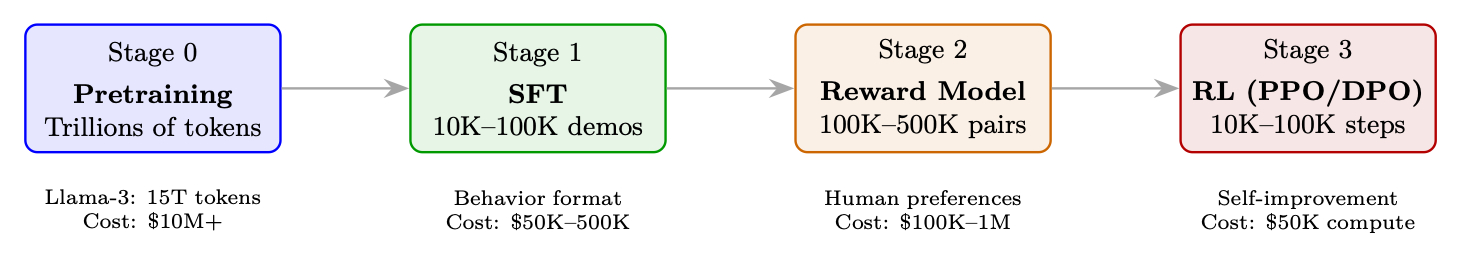
\includegraphics[width=0.85\textwidth]{figures/fig_025_fig25.png}
\end{figure}

\begin{examplebox}[Concrete PPO Step for a 70B Chat Model]
\textbf{Setup}: Batch of 128 prompts, Llama-3-70B policy, 512 max tokens.

\textbf{Step 1 --- Generate}: Sample 128 responses (temperature=0.7, top-p=0.9). This takes 60\% of time.

\textbf{Step 2 --- Score}: Reward model scores each (prompt, response) pair. Range: 0.2--0.95.

\textbf{Step 3 --- KL}: Compute per-token KL: $\text{KL}_t = \log\pi_\theta(y_t|y_{<t}) - \log\pi_\text{ref}(y_t|y_{<t})$. Mean KL across tokens: typically 3--8.

\textbf{Step 4 --- Final reward}: $R = r_\text{RM} - 0.05 \times \text{mean\_KL}$ (only at last token).

\textbf{Step 5 --- GAE}: Compute $\hat{A}_t$ for each token position using value head predictions. Whiten advantages (zero mean, unit variance).

\textbf{Step 6 --- Update}: 4 epochs of SGD on mini-batches of 16. Clip ratio $\epsilon = 0.2$. Gradient norm clipping at 1.0.

\textbf{Result}: Policy improves by $\sim$0.005 win-rate per step. After 10K steps: 5--10\% absolute improvement over SFT.
\end{examplebox}

\begin{warningbox}[Tokenization Pitfalls in RL for LLMs]
When computing per-token KL penalties and advantages, remember that tokenization determines what a ``step'' is. A single conceptual action (e.g., outputting ``2024'') might span 1--4 tokens depending on the tokenizer. This creates subtle issues:

\begin{itemize}
  \item \textbf{KL accounting}: Per-token KL sums to different totals for the same semantic content tokenized differently (e.g., rare words split into more subwords get higher total KL penalty).
  \item \textbf{Credit assignment}: GAE assigns advantage per token position---but semantic ``decisions'' often span multiple tokens. The model only truly ``decides'' at the first token of a word; subsequent subword tokens are largely deterministic.
  \item \textbf{Reward placement}: Placing reward only at the final token means all preceding tokens must propagate credit backward through GAE---longer responses suffer from more diluted signal.
\end{itemize}

\textbf{Mitigation}: Some systems normalize KL by sequence length, use word-level reward shaping, or apply reward at semantic boundaries rather than the final token.
\end{warningbox}

\section{Detailed Mechanics: Logits and Policy Updates}
\label{detailed-mechanics-logits-and-policy-updates}

\begin{figure}[ht!]
\centering
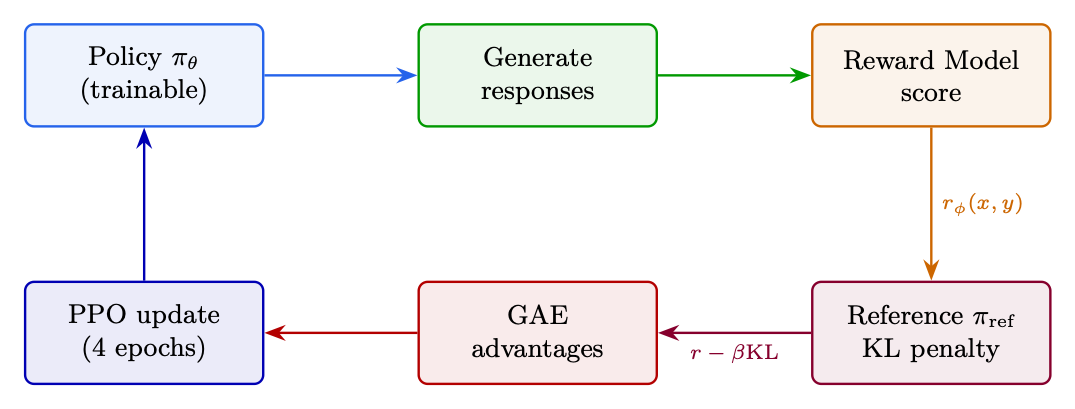
\includegraphics[width=0.85\textwidth]{figures/fig_026_fig26.png}
\caption{PPO end-to-end: from prompt batch through generation, reward scoring, KL computation, advantage estimation, to clipped policy update. The feedback loop shows the updated policy being used for the next generation step.}
\end{figure}

PPO manages two distinct parameter states in memory, which share the same neural network topology but hold different weight values during optimization:

\begin{keybox}[Core Architecture: Two Networks]
\begin{enumerate}
  \item \textbf{The Policy Network ($\pi_\theta$):} The active, live network parameterized by weights $\theta$. Continuously updated via backpropagation during optimization.
  \item \textbf{The Old Policy Network ($\pi_{\theta_{\text{old}}}$):} A frozen snapshot parameterized by weights $\theta_{\text{old}}$. Acts as a static anchor during a single optimization cycle to prevent the policy from shifting too drastically.
\end{enumerate}
\end{keybox}

\subsection{Phase 1: Rollout (Data Collection)}
\label{phase-1-rollout-data-collection}

During data collection, the agent interacts with the environment for $T$ steps. At each time-step $t$:

\begin{enumerate}
  \item The environment yields the current state/observation $s_t$ (for LLMs: prompt + tokens generated so far).
  \item State $s_t$ is passed through the current network snapshot ($\theta_{\text{old}}$).
  \item The network outputs raw unnormalized values --- \textbf{logits} $z_{\text{old}}$ --- a vector of size $|V|$ (vocabulary size 32K--128K).
  \item Probabilities are computed via Softmax: 
\begin{equation}
\boxed{P(a \mid s_t) = \text{Softmax}(z_{\text{old}}) = \frac{\exp(z_{\text{old}, a})}{\sum_{j=1}^{|V|} \exp(z_{\text{old}, j})}}
\end{equation}
  \item An action $a_t$ (next token) is sampled from $P(a \mid s_t)$, and the transition tuple $\langle s_t, a_t, r_t, s_{t+1} \rangle$ along with $\log \pi_{\theta_{\text{old}}}(a_t \mid s_t)$ is stored in the rollout buffer.
\end{enumerate}

\begin{intuitionbox}[Why Store Log-Probabilities?]
Storing $\log \pi_{\theta_{\text{old}}}(a_t \mid s_t)$ as a scalar during rollout avoids re-running the frozen network during optimization. This saves one full forward pass per mini-batch --- significant for 70B models.
\end{intuitionbox}

\subsection{Phase 2: Optimization Loop (Mini-Batch Updates)}
\label{phase-2-optimization-loop-mini-batch-updates}

Once the rollout buffer is full, PPO runs $K$ epochs (typically 3--10) over mini-batches. For every gradient step, logits are generated for both policies using the stored state $s_t$:

\textbf{Old Policy Evaluation} (frozen): 
\begin{equation}
z_{\text{old}} = f(s_t; \theta_{\text{old}}) \quad \longrightarrow \quad \log \pi_{\theta_{\text{old}}}(a_t \mid s_t) = \text{LogSoftmax}(z_{\text{old}})[a_t]
\end{equation}

\emph{Implementation shortcut: reuse the stored scalar from rollout instead of re-computing.}

\textbf{Live Policy Evaluation} (updating): 
\begin{equation}
z_{\text{new}} = f(s_t; \theta) \quad \longrightarrow \quad \log \pi_\theta(a_t \mid s_t) = \text{LogSoftmax}(z_{\text{new}})[a_t]
\end{equation}

Because $\theta$ updates after every mini-batch gradient step, $z_{\text{new}}$ changes continuously throughout the optimization loop, whereas $z_{\text{old}}$ remains perfectly static.

\subsection{From Logits to Probability Ratio}
\label{from-logits-to-probability-ratio}

The core PPO ratio measures how much more or less likely an action is under the new policy vs the old: 
\begin{equation}
\boxed{r_t(\theta) = \frac{\pi_\theta(a_t \mid s_t)}{\pi_{\theta_{\text{old}}}(a_t \mid s_t)}}
\end{equation}

To avoid catastrophic numerical underflow/overflow from dividing raw probabilities, the calculation is performed in \textbf{log-space}: 
\begin{align}
\log \pi_\theta(a_t \mid s_t) &= \text{LogSoftmax}(z_{\text{new}})[a_t] \\
\log \pi_{\theta_{\text{old}}}(a_t \mid s_t) &= \text{LogSoftmax}(z_{\text{old}})[a_t]
\end{align}

The ratio is recovered via exponentiation of the difference: 
\begin{equation}
\boxed{r_t(\theta) = \exp\!\left(\log \pi_\theta(a_t \mid s_t) - \log \pi_{\theta_{\text{old}}}(a_t \mid s_t)\right)}
\end{equation}

This ratio is injected into the PPO clipping objective: 
\begin{equation}
\boxed{\mathcal{L}^{\text{CLIP}}(\theta) = \hat{\mathbb{E}}_t \left[ \min\!\left(r_t(\theta)\hat{A}_t, \;\text{clip}(r_t(\theta),\, 1{-}\epsilon,\, 1{+}\epsilon)\,\hat{A}_t\right) \right]}
\end{equation}

\begin{intuitionbox}[How Clipping Works]
\begin{itemize}
  \item If $\hat{A}_t > 0$ (good action): ratio is clipped at $1+\epsilon$ --- cannot over-exploit good actions.
  \item If $\hat{A}_t < 0$ (bad action): ratio is clipped at $1-\epsilon$ --- cannot over-penalize bad actions.
  \item The $\min(\cdot)$ ensures we always take the more conservative estimate.
\end{itemize}

Result: monotonic improvement within a trust region --- no catastrophic collapses.
\end{intuitionbox}

\subsection{The PPO Weight Lifecycle}
\label{the-ppo-weight-lifecycle}

\begin{table}[ht!]
\centering
\caption{Evolution of $\theta$ and $\theta_{\text{old}}$ across PPO training phases.}
\begin{tabular}{@{}lp{3.5cm}p{3.5cm}p{6cm}@{}}
\toprule
\textbf{Phase} & \textbf{Live $\theta$} & \textbf{Old $\theta_{\text{old}}$} & \textbf{Ratio $r_t(\theta)$} \\
\midrule
1. Rollout Start & Active copy & Same active copy & Always $1.0$ (by identity) \\
2. Batch Step 1 & Computes gradients & Frozen & $1.0$ (initial step) \\
3. Batch Step $N$ & Modifying ($\theta \neq \theta_{\text{old}}$) & Frozen & Deviates from $1.0$ (e.g., $1.06$, $0.94$) \\
4. Clipping Active & Bounded by $\epsilon$ & Frozen & Trapped at bound ($1 \pm \epsilon$) \\
5. Optimization End & Highly optimized & Discarded & N/A \\
6. Next Cycle & $\theta \rightarrow \theta_{\text{old}}$ & Receives fresh $\theta$ & Resets back to $1.0$ \\
\bottomrule
\end{tabular}
\end{table}

\subsection{Continuous Action Spaces Extension}
\label{continuous-action-spaces-extension}

For continuous action spaces (not typical for LLMs, but important for robotics RL), the network outputs distribution parameters instead of discrete logits:

\begin{itemize}
  \item Predicted mean vector $\mu$
  \item Predicted standard deviation vector $\sigma$
\end{itemize}

Log-probabilities are computed via the Gaussian log-PDF: 
\begin{equation}
\boxed{\log \pi(a_t \mid s_t) = -\frac{1}{2}\left(\frac{a_t - \mu}{\sigma}\right)^{\!2} - \log(\sigma) - \frac{1}{2}\log(2\pi)}
\end{equation}

The ratio $r_t(\theta) = \exp(\log \pi_\theta - \log \pi_{\theta_{\text{old}}})$ is then computed identically and fed into the same clipping objective.

\section{TRL Implementation}
\label{trl-implementation}

The HuggingFace TRL library~\cite{vonwerra2022trl} provides production-ready implementations of all major RL methods for LLMs.

\begin{lstlisting}[style=pythonstyle]
from trl import PPOConfig, PPOTrainer, AutoModelForCausalLMWithValueHead
from transformers import AutoTokenizer
from peft import LoraConfig

# Model setup
model = AutoModelForCausalLMWithValueHead.from_pretrained(
    "meta-llama/Llama-3.1-8B-Instruct",
    torch_dtype=torch.bfloat16, device_map="auto",
    peft_config=LoraConfig(r=64, lora_alpha=16, target_modules=["q_proj","v_proj","k_proj","o_proj"])
)
tokenizer = AutoTokenizer.from_pretrained("meta-llama/Llama-3.1-8B-Instruct")

# PPO config with all critical hyperparameters
ppo_config = PPOConfig(
    learning_rate=1.5e-6,        # Low LR for stability
    batch_size=128,              # Prompts per step
    mini_batch_size=16,          # Gradient accumulation unit
    ppo_epochs=4,                # Epochs per batch (reuse data)
    gamma=1.0,                   # No discounting (single turn)
    lam=0.95,                    # GAE lambda
    cliprange=0.2,               # PPO epsilon
    cliprange_value=0.2,         # Value function clipping
    vf_coef=0.1,                 # Value loss coefficient
    init_kl_coef=0.05,           # Initial KL penalty
    target_kl=6.0,               # Adaptive KL target
    whiten_rewards=True,         # Normalize advantages
    gradient_accumulation_steps=4,
    max_grad_norm=1.0,
)

ppo_trainer = PPOTrainer(config=ppo_config, model=model, tokenizer=tokenizer,
    dataset=prompt_dataset, data_collator=collator)

# Training loop
for batch in ppo_trainer.dataloader:
    # 1. Generate responses
    query_tensors = batch["input_ids"]
    response_tensors = ppo_trainer.generate(
        query_tensors, max_new_tokens=512, temperature=0.7, top_p=0.9, do_sample=True
    )
    # 2. Score with reward model
    texts = [tokenizer.decode(r, skip_special_tokens=True) for r in response_tensors]
    rewards = [torch.tensor(reward_model.score(q, r)) for q, r in zip(batch["query"], texts)]
    # 3. PPO update (handles KL, GAE, clipping internally)
    stats = ppo_trainer.step(query_tensors, response_tensors, rewards)
    # Monitor: stats["ppo/mean_scores"], stats["ppo/policy/approx_kl"]
\end{lstlisting}

\section{Critical Hyperparameters}
\label{critical-hyperparameters}

\begin{tabular}{@{}lp{5cm}p{8cm}@{}}
\toprule
\textbf{Parameter} & \textbf{Typical} & \textbf{Effect of Getting It Wrong} \\
\midrule
\texttt{cliprange} & 0.2 & Too low: no learning. Too high: instability. \\
\texttt{init\_kl\_coef} & 0.01--0.1 & Too low: reward hacking. Too high: stuck at SFT. \\
\texttt{target\_kl} & 4--8 & Adaptive controller target. Lower = conservative. \\
\texttt{ppo\_epochs} & 4 & Too many: overfits to batch. Too few: wastes gen compute. \\
\texttt{learning\_rate} & $1{-}5 \times 10^{-6}$ & Too high: catastrophic forgetting. \\
\texttt{batch\_size} & 64--256 & Larger = smoother gradients, more gen compute. \\
\texttt{temperature} & 0.7--1.0 & Lower: less exploration. Higher: noisier advantages. \\
\bottomrule
\end{tabular}

\chapter{DPO --- Direct Preference Optimization}
\label{dpo-direct-preference-optimization}

\section{Motivation}
\label{motivation}

PPO requires 4 models in memory (policy, reference, reward model, value head), complex RL infrastructure, and is notoriously unstable. DPO~\cite{rafailov2023direct} asks: \emph{can we skip the RL and learn directly from preferences?}

\textbf{Key insight}: The optimal policy under the RLHF objective (reward maximization + KL penalty) has a \textbf{closed-form solution}. We can derive a supervised loss that implicitly optimizes the same objective.

\section{Mathematical Derivation}
\label{mathematical-derivation}

\textbf{Step 1}: RLHF objective: $\max_\pi \mathbb{E}_{x,y\sim\pi}[r(x,y)] - \beta D_\text{KL}[\pi\|\pi_\text{ref}]$

\textbf{Step 2}: The optimal solution is: $\pi^*(y|x) = \frac{1}{Z(x)} \pi_\text{ref}(y|x) \exp\left(\frac{r(x,y)}{\beta}\right)$

\textbf{Step 3}: Rearrange to express reward in terms of policy: $r(x,y) = \beta \log \frac{\pi^*(y|x)}{\pi_\text{ref}(y|x)} + \beta \log Z(x)$

\textbf{Step 4}: Substitute into Bradley-Terry preference model $P(y_w \succ y_l) = \sigma(r(y_w) - r(y_l))$. The $Z(x)$ cancels!

\begin{equation}
\boxed{\mathcal{L}_\text{DPO}(\theta) = -\mathbb{E}_{(x, y_w, y_l)}\left[\log\sigma\left(\beta\log\frac{\pi_\theta(y_w|x)}{\pi_\text{ref}(y_w|x)} - \beta\log\frac{\pi_\theta(y_l|x)}{\pi_\text{ref}(y_l|x)}\right)\right]}
\end{equation}

\begin{intuitionbox}[What DPO Actually Does]
Define the \textbf{implicit reward} as $\hat{r}(x,y) = \beta\log\frac{\pi_\theta(y|x)}{\pi_\text{ref}(y|x)}$.

DPO minimizes the cross-entropy loss where the ``label'' is: chosen should have higher implicit reward than rejected. The margin is controlled by $\beta$:

\begin{itemize}
  \item Large $\beta$: need large margin $\rightarrow$ policy moves aggressively $\rightarrow$ risk forgetting
  \item Small $\beta$: small margin suffices $\rightarrow$ policy stays close to reference $\rightarrow$ conservative
\end{itemize}

The reference model acts as a regularizer: the policy must ``justify'' any deviation from it by showing preference alignment.
\end{intuitionbox}

\section{Gradient Analysis}
\label{gradient-analysis}

The DPO gradient decomposes as: 
\begin{equation}
\nabla_\theta \mathcal{L} = -\beta \cdot \underbrace{\sigma(-\hat{r}_w + \hat{r}_l)}_{\text{weight: higher when model is wrong}} \cdot \left[\nabla_\theta \log\pi_\theta(y_w|x) - \nabla_\theta \log\pi_\theta(y_l|x)\right]
\end{equation}
 \textbf{Interpretation}: The gradient increases probability of chosen and decreases rejected. The weight is largest when the model currently prefers the wrong answer --- it focuses learning on ``confusing'' pairs.

\begin{examplebox}[Concrete DPO Example]
\textbf{Prompt}: ``Explain quantum entanglement to a 10-year-old.''

\textbf{Chosen} ($y_w$): ``Imagine you have two magic coins. When you flip one and it’s heads, the other one instantly becomes tails, no matter how far apart they are!''\\

$\log\pi_\theta(y_w|x) = -15.3$, $\log\pi_\text{ref}(y_w|x) = -16.1$

\textbf{Rejected} ($y_l$): ``Quantum entanglement is a phenomenon where two particles become correlated such that the quantum state of one particle cannot be described independently.''\\

$\log\pi_\theta(y_l|x) = -12.8$, $\log\pi_\text{ref}(y_l|x) = -12.5$

\textbf{Implicit rewards}: $\hat{r}_w = 0.1 \times ((-15.3) - (-16.1)) = 0.08$, $\hat{r}_l = 0.1 \times ((-12.8) - (-12.5)) = -0.03$

\textbf{Loss input}: $\sigma(0.08 - (-0.03)) = \sigma(0.11) = 0.527$

\textbf{Loss}: $-\log(0.527) = 0.64$ --- The model barely prefers the chosen. Gradient will push hard.

After training: chosen probability increases, rejected decreases, until margin stabilizes around $1/(2\beta)$.
\end{examplebox}

\section{TRL Implementation}
\label{trl-implementation-dup2}

The following shows a minimal working example using HuggingFace TRL.

\begin{lstlisting}[style=pythonstyle]
from trl import DPOConfig, DPOTrainer
from transformers import AutoModelForCausalLM, AutoTokenizer
from peft import LoraConfig
from datasets import load_dataset

model = AutoModelForCausalLM.from_pretrained("meta-llama/Llama-3.1-8B-Instruct",
    torch_dtype=torch.bfloat16, attn_implementation="flash_attention_2")
tokenizer = AutoTokenizer.from_pretrained("meta-llama/Llama-3.1-8B-Instruct")

# Dataset format: {"prompt": str, "chosen": str, "rejected": str}
dataset = load_dataset("argilla/ultrafeedback-binarized-preferences")

lora_config = LoraConfig(r=64, lora_alpha=16, lora_dropout=0.05,
    target_modules=["q_proj","k_proj","v_proj","o_proj","gate_proj","up_proj","down_proj"])

dpo_config = DPOConfig(
    output_dir="./dpo_output",
    beta=0.1,                    # KL regularization strength
    learning_rate=5e-7,          # Very low LR for stability
    loss_type="sigmoid",         # Standard DPO loss
    max_length=2048,             # Max sequence length
    max_prompt_length=1024,      # Truncation for prompts
    per_device_train_batch_size=2,
    gradient_accumulation_steps=8,  # Effective batch = 16
    gradient_checkpointing=True,
    bf16=True,
    num_train_epochs=1,          # DPO overfits fast - 1 epoch!
    warmup_ratio=0.1,
    logging_steps=10,
    eval_strategy="steps",
    eval_steps=200,
    save_strategy="steps",
    save_steps=500,
)

trainer = DPOTrainer(
    model=model,
    ref_model=None,             # With LoRA, ref = base model (no copy needed!)
    args=dpo_config,
    train_dataset=dataset["train"],
    eval_dataset=dataset["test"],
    tokenizer=tokenizer,
    peft_config=lora_config,
)
trainer.train()
# Key metrics to monitor: train/rewards/chosen, train/rewards/rejected, train/rewards/margins
\end{lstlisting}

\section{How DPO Works: Full Mechanics}
\label{how-dpo-works-full-mechanics}

This section provides the complete computational details of DPO --- what happens at the token level during training.

\subsection{Sequence-Level Log-Probabilities}
\label{sequence-level-log-probabilities}

The key quantity in DPO is the log-probability of an \textbf{entire sequence} $y = (y_1, y_2, \ldots, y_T)$ given prompt $x$. This is computed as the \textbf{sum of per-token log-probabilities}:

\begin{equation}
\boxed{\log \pi_\theta(y|x) = \sum_{t=1}^{T} \log \pi_\theta(y_t \mid x, y_{<t})}
\end{equation}

Each term $\log \pi_\theta(y_t | x, y_{<t})$ is the log-softmax output at position $t$ for the \emph{actual} token $y_t$ in the sequence. This is identical to the cross-entropy loss used in standard language modeling --- but here we \textbf{sum} rather than average.

\textbf{Critical detail}: The gradient flows through \textbf{every token position} in both $y_w$ and $y_l$. There is no masking of intermediate tokens --- every token contributes to the sequence-level log-probability.

\subsection{The DPO Loss Decomposed}
\label{the-dpo-loss-decomposed}

Starting from the loss: 
\begin{equation}
\mathcal{L}_{\text{DPO}}(\theta) = -\mathbb{E}_{(x, y_w, y_l) \sim \mathcal{D}}\!\left[\log \sigma\!\left(\beta \cdot h_\theta(x, y_w, y_l)\right)\right]
\end{equation}
 where the ``implicit reward margin'' $h_\theta$ is: 
\begin{equation}
h_\theta(x, y_w, y_l) = \underbrace{\log \frac{\pi_\theta(y_w|x)}{\pi_{\text{ref}}(y_w|x)}}_{\text{chosen reward proxy}} - \underbrace{\log \frac{\pi_\theta(y_l|x)}{\pi_{\text{ref}}(y_l|x)}}_{\text{rejected reward proxy}}
\end{equation}

Expanding into token-level terms: 
\begin{equation}
\boxed{h_\theta = \sum_{t=1}^{|y_w|}\!\left[\log\pi_\theta(y_w^t | x, y_w^{<t}) - \log\pi_{\text{ref}}(y_w^t | x, y_w^{<t})\right] - \sum_{t=1}^{|y_l|}\!\left[\log\pi_\theta(y_l^t | x, y_l^{<t}) - \log\pi_{\text{ref}}(y_l^t | x, y_l^{<t})\right]}
\end{equation}

\subsection{Forward Pass: Step by Step}
\label{forward-pass-step-by-step}

For one training example $(x, y_w, y_l)$:

\begin{enumerate}
  \item \textbf{Concatenate}: Form two sequences: $[x; y_w]$ and $[x; y_l]$. Pad to equal length within the batch.
  \item \textbf{Forward pass (policy $\pi_\theta$)}: Run both sequences through the model. Collect logits at every response position.
  \item \textbf{Extract log-probs}: At each position $t$ in the response, take $\log\text{softmax}(\text{logits}_t)[y_t]$ --- the log-probability of the actual token.
  \item \textbf{Sum over tokens}: 
\begin{align}
\text{logp\_chosen} &= \sum_{t \in \text{response positions}} \log\pi_\theta(y_w^t | x, y_w^{<t}) \\
\text{logp\_rejected} &= \sum_{t \in \text{response positions}} \log\pi_\theta(y_l^t | x, y_l^{<t})
\end{align}
  \item \textbf{Subtract reference} (pre-computed or from second forward pass): 
\begin{align}
\text{ratio\_w} &= \text{logp\_chosen} - \text{ref\_logp\_chosen} \\
\text{ratio\_l} &= \text{logp\_rejected} - \text{ref\_logp\_rejected}
\end{align}
  \item \textbf{Compute loss}: $\mathcal{L} = -\log\sigma(\beta \cdot (\text{ratio\_w} - \text{ratio\_l}))$
  \item \textbf{Backward pass}: Gradients flow back through steps 5 $\rightarrow$ 4 $\rightarrow$ 3 $\rightarrow$ 2 to update $\theta$.
\end{enumerate}

\subsection{Token-Level Gradient Analysis}
\label{token-level-gradient-analysis}

\textbf{Does every token get a gradient?} Yes. The gradient with respect to the logits at position $t$ in the chosen sequence is:

\begin{equation}
\frac{\partial \mathcal{L}}{\partial \text{logits}_t^{(w)}} = -\underbrace{\sigma(-\beta \cdot h_\theta)}_{\text{scaling factor}} \cdot \beta \cdot \frac{\partial \log\pi_\theta(y_w^t | \cdot)}{\partial \text{logits}_t^{(w)}}
\end{equation}

\textbf{Key insight}: The scaling factor $\sigma(-\beta \cdot h_\theta)$ is \textbf{shared across all tokens} in both sequences. It acts as an adaptive learning rate:

\begin{itemize}
  \item When $h_\theta$ is small (model can’t distinguish chosen from rejected): scaling $\approx 0.5$ --- strong gradient, learn aggressively.
  \item When $h_\theta$ is large (model already prefers chosen): scaling $\approx 0$ --- negligible gradient, don’t over-fit.
\end{itemize}

\textbf{Effect on chosen tokens}: Probability is \emph{increased} (log-prob pushed up).\\

\textbf{Effect on rejected tokens}: Probability is \emph{decreased} (log-prob pushed down).\\

\textbf{Relative to reference}: Only the \emph{difference} from $\pi_{\text{ref}}$ matters. If the model already assigns high probability to the chosen response (matching the reference), there’s little gradient.

\subsection{Per-Token vs. Sequence-Level: Length Normalization}
\label{per-token-vs.-sequence-level-length-normalization}

A subtle issue: longer sequences naturally have lower log-probabilities (more terms summed, each $\leq 0$). If $|y_w| \gg |y_l|$, the loss can be biased toward preferring shorter responses.

\textbf{Solutions}:

\begin{itemize}
  \item \textbf{Length-normalized DPO}: Replace $\log\pi_\theta(y|x)$ with $\frac{1}{|y|}\sum_t \log\pi_\theta(y_t|\cdot)$. Used in some implementations (SimPO adopts this).
  \item \textbf{Standard DPO}: Uses raw sum (no normalization). This \emph{implicitly} penalizes verbosity --- the model must assign high probability to every token in the chosen response.
  \item \textbf{Practical impact}: On benchmarks, length-normalized DPO reduces length gaming but can hurt instruction-following quality. Standard (unnormalized) is more common in production.
\end{itemize}

\subsection{Label Masking: What Gets Gradients}
\label{label-masking-what-gets-gradients}

\begin{keybox}[Which Tokens Receive Gradient in DPO]
\begin{itemize}
  \item \textbf{Prompt tokens} ($x$): \textbf{NO gradient}. The loss is computed only over response positions. Prompt tokens provide context but their logits don’t contribute to $\log\pi(y|x)$.
  \item \textbf{Chosen response tokens} ($y_w$): \textbf{ALL tokens get gradient}. Each $y_w^t$ contributes to the sum. Gradient pushes their probabilities up.
  \item \textbf{Rejected response tokens} ($y_l$): \textbf{ALL tokens get gradient}. Each $y_l^t$ contributes to the sum. Gradient pushes their probabilities down.
  \item \textbf{Padding tokens}: \textbf{NO gradient}. Masked out with attention mask.
\end{itemize}
\end{keybox}

\subsection{Pseudocode: DPO Training Step}
\label{pseudocode-dpo-training-step}

\begin{examplebox}[DPO Forward + Backward (PyTorch-style)]
\begin{lstlisting}[style=pythonstyle]
def dpo_loss(model, ref_model, batch, beta=0.1):
    """One DPO training step."""
    # batch contains: input_ids_chosen, input_ids_rejected,
    #                 labels_chosen, labels_rejected (prompt masked to -100)
    
    # 1. Forward pass: get per-token log-probs
    logps_chosen = get_sequence_logprob(model, batch["chosen"])
    logps_rejected = get_sequence_logprob(model, batch["rejected"])
    
    # 2. Reference log-probs (pre-computed or computed here)
    with torch.no_grad():
        ref_logps_chosen = get_sequence_logprob(ref_model, batch["chosen"])
        ref_logps_rejected = get_sequence_logprob(ref_model, batch["rejected"])
    
    # 3. Compute implicit reward margins
    chosen_rewards = beta * (logps_chosen - ref_logps_chosen)
    rejected_rewards = beta * (logps_rejected - ref_logps_rejected)
    
    # 4. DPO loss = -log(sigmoid(chosen_reward - rejected_reward))
    loss = -F.logsigmoid(chosen_rewards - rejected_rewards).mean()
    return loss

def get_sequence_logprob(model, sequences):
    """Sum of log-probs over response tokens only."""
    outputs = model(sequences["input_ids"], attention_mask=sequences["mask"])
    logits = outputs.logits[:, :-1, :]  # Shift for next-token prediction
    
    # Gather log-prob of actual tokens
    labels = sequences["labels"][:, 1:]  # Shifted labels
    log_probs = F.log_softmax(logits, dim=-1)
    token_logps = log_probs.gather(-1, labels.unsqueeze(-1)).squeeze(-1)
    
    # Mask: only sum over response tokens (labels != -100)
    mask = (labels != -100).float()
    return (token_logps * mask).sum(dim=-1)  # Shape: [batch_size]
\end{lstlisting}
\end{examplebox}

\subsection{Common Pitfalls}
\label{common-pitfalls}

\begin{warningbox}[DPO Implementation Pitfalls]
\begin{itemize}
  \item \textbf{Forgetting to mask the prompt}: If prompt tokens are included in the log-prob sum, the model optimizes for prompt likelihood (useless) and the effective $\beta$ is wrong.
  \item \textbf{Using mean instead of sum}: $\frac{1}{T}\sum_t \log\pi$ vs. $\sum_t \log\pi$ --- these give different implicit length penalties. Must be consistent between $\pi_\theta$ and $\pi_{\text{ref}}$.
  \item \textbf{Stale reference model}: If $\pi_{\text{ref}}$ is too far from $\pi_\theta$ (e.g., base model vs. fine-tuned), the KL term dominates and gradients vanish. Solution: use the SFT checkpoint (not base) as reference.
  \item \textbf{$\beta$ too large}: Magnifies log-prob differences $\rightarrow$ sigmoid saturates $\rightarrow$ zero gradients. Start with $\beta = 0.1$, tune in $[0.05, 0.5]$.
  \item \textbf{$\beta$ too small}: Theoretically allows more freedom from reference (weaker KL constraint), but the gradient $\propto \beta \cdot \sigma(-\beta h)$ becomes vanishingly small $\rightarrow$ loss landscape is flat $\rightarrow$ extremely slow convergence. The model has ``permission'' to move far but receives almost no signal telling it \emph{where} to move.
\end{itemize}
\end{warningbox}

\section{DPO Variants and When Each Fails}
\label{dpo-variants-and-when-each-fails}

\begin{warningbox}[When DPO Fails]
\textbf{1. Distribution shift}: Preference data from old model. Current policy generates different text $\rightarrow$ loss is optimizing on irrelevant examples.

\textbf{2. No exploration}: Can’t discover behaviors not in dataset. Stuck in local optimum.

\textbf{3. Reference collapse}: If reference is too strong, policy can’t move. If too weak, no regularization.

\textbf{4. Data quality}: Noisy labels poison training. Unlike PPO which averages over many samples, DPO memorizes individual pairs.

\textbf{5. Preference data diversity}: Ensure chosen/rejected pairs cover the full spectrum of quality differences (not just good-vs-terrible). Pairs that differ in \emph{approach}, not just quality, teach richer policy distinctions.
\end{warningbox}

\section{\texorpdfstring{$\beta$ Selection Guide}{beta Selection Guide}}
\label{beta-selection-guide}

\begin{tabular}{@{}lp{5cm}p{8cm}@{}}
\toprule
$\beta$ & \textbf{Regime} & \textbf{When to Use} \\
\midrule
0.01 & Very aggressive & Only if data is extremely clean and you need large distributional shift \\
0.05 & Aggressive & Good data, want noticeable improvement over SFT \\
0.1 & Standard & Default starting point. Good balance of quality vs stability \\
0.2 & Conservative & Noisy data, or model already close to desired behavior \\
0.5 & Very conservative & Safety fine-tuning where you must not break capabilities \\
\bottomrule
\end{tabular}

\section{DPO Batch Size Configuration and Scaling}
\label{dpo-batch-size-configuration-and-scaling}

Unlike standard SFT which operates on single-sequence token predictions, DPO leverages a \textbf{pairwise loss} comparing a preferred sequence against a dispreferred sequence. This fundamentally alters memory utilization and optimization stability.

\subsection{Global Batch Size Target}
\label{global-batch-size-target}

Empirical evidence across DPO implementations establishes an optimal global batch size range: 
\begin{equation}
\boxed{B_{\text{global}} \in [32, 128]}
\end{equation}

\begin{itemize}
  \item $B_{\text{global}} < 32$: Severe gradient noise in implicit reward estimation $\rightarrow$ policy oscillates destructively between alignment goals (helpfulness vs. safety).
  \item $B_{\text{global}} > 128$: Diminishing returns on convergence velocity; high communication overhead across distributed compute.
\end{itemize}

\subsection{Mathematical Decomposition}
\label{mathematical-decomposition}

Because DPO loads \textbf{two} model copies simultaneously (active policy $\pi_\theta$ + frozen reference $\pi_{\text{ref}}$), per-sequence memory is doubled. The global batch size is decomposed as: 
\begin{equation}
\boxed{B_{\text{global}} = B_{\text{micro}} \times N_{\text{GPUs}} \times K_{\text{accum}}}
\end{equation}

\begin{itemize}
  \item $B_{\text{micro}}$: Per-device micro-batch size (preference pairs per forward pass).
  \item $N_{\text{GPUs}}$: Number of parallel data-processing devices.
  \item $K_{\text{accum}}$: Gradient accumulation steps before weight update.
\end{itemize}

\textbf{The pairing multiplier}: A single DPO data instance contains a prompt ($x$), chosen ($y_w$), and rejected ($y_l$). The actual tensor load per micro-batch: 
\begin{equation}
T_{\text{sequences}} = 2 \times B_{\text{micro}}
\end{equation}

For models $>$7B parameters on 80GB GPUs with context lengths 4096--8192 tokens, the physical limit is rigidly constrained to $B_{\text{micro}} \in [1, 2]$.

\subsection{Distributed Scaling Configurations}
\label{distributed-scaling-configurations}

\begin{table}[ht!]
\centering
\caption{Distributed scaling profiles for DPO training ($B_{\text{global}} = 64$ target).}
\begin{tabular}{@{}lp{5cm}p{8cm}@{}}
\toprule
\textbf{Configuration} & \textbf{Single GPU} & \textbf{8-GPU Node} \\
\midrule
$B_{\text{global}}$ & 64 & 64 \\
$B_{\text{micro}}$ & 2 (4 sequences) & 2 (4 sequences) \\
$N_{\text{GPUs}}$ & 1 & 8 \\
$K_{\text{accum}}$ & 32 steps & 4 steps \\
Throughput & Sequential/slow & High parallel throughput \\
\bottomrule
\end{tabular}
\end{table}

\subsection{VRAM Optimization: Pre-computing Reference Log-Probabilities}
\label{vram-optimization-pre-computing-reference-log-probabilities}

The DPO loss: 
\begin{equation}
\mathcal{L}_{\text{DPO}}(\theta) = -\mathbb{E}_{(x, y_w, y_l)}\!\left[\log \sigma\!\left(\beta \log \frac{\pi_\theta(y_w|x)}{\pi_{\text{ref}}(y_w|x)} - \beta \log \frac{\pi_\theta(y_l|x)}{\pi_{\text{ref}}(y_l|x)}\right)\right]
\end{equation}

Because $\pi_{\text{ref}}$ is \textbf{completely static} throughout training, its outputs can be pre-computed:

\begin{keybox}[Reference Model Eviction Strategy]
\begin{enumerate}
  \item Execute a forward pass over dataset $\mathcal{D}$ using only $\pi_{\text{ref}}$ before training begins.
  \item Cache the scalars $\log \pi_{\text{ref}}(y_w|x)$ and $\log \pi_{\text{ref}}(y_l|x)$ to disk.
  \item \textbf{Evict $\pi_{\text{ref}}$ completely from GPU memory.}
\end{enumerate}

\textbf{Result}: Available GPU memory doubles $\rightarrow$ can increase $B_{\text{micro}}$ from 1--2 to 4--8, maximizing hardware utilization and training throughput.

\emph{Implementation}: In TRL, set \texttt{precompute\_ref\_log\_probs=True} in \texttt{DPOConfig}. For 70B models, this saves $\sim$140GB of GPU memory across the cluster.
\end{keybox}

\section{DPO Extensions and Variants}
\label{sec:dpo-variants}

Direct Preference Optimization (DPO) reformulates RLHF as a supervised learning problem by deriving a closed-form mapping between the reward function and the optimal policy. The standard DPO loss is:

\[
\mathcal{L}_{\text{DPO}}(\theta) = -\mathbb{E}_{(q,y_w,y_l)}\!\left[
    \log \sigma\!\left(
      \beta \log \frac{\pi_\theta(y_w|q)}{\pi_{\text{ref}}(y_w|q)}
      - \beta \log \frac{\pi_\theta(y_l|q)}{\pi_{\text{ref}}(y_l|q)}
    \right)
  \right],
\]

where $y_w$ is the preferred (winning) response, $y_l$ is the dispreferred (losing) response, and $\beta$ controls the strength of the KL penalty. The following subsections cover the most important extensions and variants.

\subsection{f-DPO -- Generalised f-Divergence DPO}
\label{sec:fdpo}

\begin{intuitionbox}[Beyond Reverse KL]
Standard DPO uses reverse KL divergence as the regulariser between policy and reference. Reverse KL is \emph{mode-seeking}: it prefers to concentrate probability mass on a few high-reward responses. Forward KL is \emph{mode-covering}: it spreads probability mass to cover all plausible responses. f-DPO~\cite{wang2023fdpo} generalises to any f-divergence, allowing practitioners to trade off these behaviours.
\end{intuitionbox}

The f-DPO loss replaces the log-ratio with the derivative of the f-divergence generator:

\[
\mathcal{L}_{f\text{-DPO}} = -\mathbb{E}\!\left[
    f'\!\left(\frac{\pi_\theta(y_w|q)}{\pi_{\text{ref}}(y_w|q)}\right)
    - f'\!\left(\frac{\pi_\theta(y_l|q)}{\pi_{\text{ref}}(y_l|q)}\right)
  \right],
\]

where $f'$ is the derivative of the f-divergence generator function.

\begin{keybox}[f-Divergence Options in TRL]
\begin{itemize}
  \item \textbf{reverse\_kl}: $f'(u) = \log u$. Standard DPO. Mode-seeking.
  \item \textbf{forward\_kl}: $f'(u) = -1/u$. Mode-covering. Better diversity.
  \item \textbf{js\_divergence}: $f'(u) = \log(2u/(u+1))$. Balanced mode-seeking/covering.
  \item \textbf{alpha\_divergence}: $f'(u) = u^{\alpha-1}$. Interpolates between forward and reverse KL.
\end{itemize}
\end{keybox}

\begin{examplebox}[f-DPO in TRL]
\begin{lstlisting}[style=pythonstyle]
from trl import DPOConfig, DPOTrainer

# Jensen-Shannon divergence (balanced)
config = DPOConfig(
    f_divergence_type="js_divergence",
    beta=0.1,
)

# Alpha divergence (alpha=0: forward KL, alpha=1: reverse KL)
config_alpha = DPOConfig(
    f_divergence_type="alpha_divergence",
    f_alpha_divergence_coef=0.5,   # alpha parameter
    beta=0.1,
)

trainer = DPOTrainer(
    model=model,
    ref_model=ref_model,
    args=config,
    train_dataset=dataset,
)
\end{lstlisting}
\end{examplebox}

\begin{keybox}[When to Use f-DPO]
\begin{itemize}
  \item Use \textbf{JS divergence} when you want a balance between diversity and quality.
  \item Use \textbf{forward KL} for creative tasks where diversity is paramount.
  \item Use \textbf{reverse KL} (standard DPO) for tasks with a single correct answer.
  \item Use \textbf{alpha divergence} to continuously interpolate and tune the trade-off.
\end{itemize}
\end{keybox}

\subsection{Robust DPO}
\label{sec:robust-dpo}

\begin{intuitionbox}[Noisy Labels in Preference Data]
Human preference annotations are noisy. Annotators disagree, make mistakes, and sometimes flip the preferred/dispreferred labels. Standard DPO treats all labels as ground truth, which can cause the model to overfit to noise. Robust DPO~\cite{chowdhury2024robustdpo} analytically debiases the loss under a known noise model.
\end{intuitionbox}

Assume each label is flipped with probability $\epsilon$ (the noise rate). The debiased loss is:

\[
\boxed{
    \mathcal{L}_{\text{robust}} =
    \frac{(1-\epsilon)\,\mathcal{L}_{\text{DPO}}(y_w, y_l)
          - \epsilon\,\mathcal{L}_{\text{DPO}}(y_l, y_w)}{1 - 2\epsilon},
  }
\]

where $\mathcal{L}_{\text{DPO}}(y_w, y_l)$ is the standard DPO loss treating $y_w$ as preferred, and $\mathcal{L}_{\text{DPO}}(y_l, y_w)$ is the loss with labels flipped. This correction removes the bias introduced by label noise.

\begin{keybox}[Intuition for Robust DPO]
The formula is a linear combination that ``subtracts out'' the contribution of flipped labels. When $\epsilon=0$, it reduces to standard DPO. When $\epsilon=0.5$, the denominator goes to zero -- the labels are pure noise and no learning is possible. In practice, $\epsilon \in [0.05, 0.2]$ covers most real annotation noise levels.
\end{keybox}

\begin{examplebox}[Robust DPO in TRL]
\begin{lstlisting}[style=pythonstyle]
from trl import DPOConfig, DPOTrainer

config = DPOConfig(
    loss_type="robust",
    label_smoothing=0.1,   # corresponds to epsilon = 0.1
    beta=0.1,
)

trainer = DPOTrainer(
    model=model,
    ref_model=ref_model,
    args=config,
    train_dataset=dataset,
)
\end{lstlisting}
\end{examplebox}

\subsection{TR-DPO -- Trust Region DPO}
\label{sec:tr-dpo}

\begin{intuitionbox}[Stale Reference Model Problem]
Standard DPO uses a fixed reference model $\pi_{\text{ref}}$ throughout training. As the policy $\pi_\theta$ improves, the KL penalty $\beta \log(\pi_\theta/\pi_{\text{ref}})$ grows, eventually dominating the loss and preventing further improvement. TR-DPO~\cite{gorbatenko2024trdpo} periodically updates the reference model to track the current policy.
\end{intuitionbox}

TR-DPO updates the reference model using an exponential moving average (EMA):

\[
\pi_{\text{ref}}^{(t+1)} \leftarrow
    \alpha \cdot \pi_\theta^{(t)} + (1-\alpha) \cdot \pi_{\text{ref}}^{(t)},
\]

where $\alpha \in (0,1)$ is the mixup coefficient. This is applied every $T_{\text{sync}}$ gradient steps.

\begin{examplebox}[TR-DPO in TRL]
\begin{lstlisting}[style=pythonstyle]
from trl import DPOConfig, DPOTrainer

config = DPOConfig(
    loss_type="sigmoid",        # standard DPO loss
    sync_ref_model=True,        # enable TR-DPO
    ref_model_mixup_alpha=0.6,  # alpha: how much of current policy to mix in
    ref_model_sync_steps=512,   # T_sync: sync every 512 steps
    beta=0.1,
)

trainer = DPOTrainer(
    model=model,
    ref_model=ref_model,
    args=config,
    train_dataset=dataset,
)
\end{lstlisting}
\end{examplebox}

\begin{keybox}[When to Use TR-DPO]
\begin{itemize}
  \item Long training runs where the policy drifts far from the initial reference.
  \item When you observe the DPO loss plateauing early due to KL penalty domination.
  \item Iterative DPO pipelines where new preference data is collected from the current policy.
  \item Set $\alpha$ close to 1 for fast reference updates; close to 0 for slow updates.
\end{itemize}
\end{keybox}

\subsection{EXO -- Exact Optimisation}
\label{sec:exo}

\begin{intuitionbox}[DPO’s KL Direction Problem]
DPO is derived by solving for the optimal policy under a reverse KL constraint. However, the resulting loss actually optimises a \emph{forward} KL objective in the reward space, which is the wrong direction. EXO~\cite{ji2024exo} corrects this by using reverse KL probability matching, which is the theoretically correct objective for alignment.
\end{intuitionbox}

EXO minimises the reverse KL between the model distribution and the target (reward-optimal) distribution:

\[
\mathcal{L}_{\text{EXO}} = \mathbb{E}_{y \sim \pi_\theta}\!\left[
    \log \frac{\pi_\theta(y|q)}{p^*(y|q)}
  \right],
\]

where $p^*(y|q) \propto \pi_{\text{ref}}(y|q) \exp(r(y,q)/\beta)$ is the optimal policy. In practice, EXO approximates this using the available preference pairs:

\[
\mathcal{L}_{\text{EXO}} \approx -\mathbb{E}\!\left[
    \log \sigma\!\left(
      \beta \log \frac{\pi_{\text{ref}}(y_w|q)}{\pi_\theta(y_w|q)}
      - \beta \log \frac{\pi_{\text{ref}}(y_l|q)}{\pi_\theta(y_l|q)}
    \right)
  \right].
\]

Note the \emph{swapped} roles of $\pi_\theta$ and $\pi_{\text{ref}}$ compared to DPO.

\begin{examplebox}[EXO in TRL]
\begin{lstlisting}[style=pythonstyle]
from trl import DPOConfig, DPOTrainer

config = DPOConfig(
    loss_type="exo_pair",
    beta=0.1,
)

trainer = DPOTrainer(
    model=model,
    ref_model=ref_model,
    args=config,
    train_dataset=dataset,
)
\end{lstlisting}
\end{examplebox}

\subsection{NCA -- Noise Contrastive Alignment}
\label{sec:nca}

\begin{intuitionbox}[Likelihood Collapse in DPO]
A known failure mode of DPO is \emph{likelihood collapse}: the model learns to decrease the probability of the losing response but also decreases the probability of the winning response (since the loss only cares about the \emph{difference}). NCA~\cite{chen2024nca} adds an absolute likelihood term to prevent this.
\end{intuitionbox}

NCA reframes alignment as noise-contrastive estimation. The loss has three terms:

\[
\boxed{
    \mathcal{L}_{\text{NCA}} =
      -\log \sigma(r_w)
      - \tfrac{1}{2}\log \sigma(-r_w)
      - \tfrac{1}{2}\log \sigma(-r_l),
  }
\]

where $r_y = \beta \log(\pi_\theta(y|q)/\pi_{\text{ref}}(y|q))$ is the implicit reward. The first term encourages high reward for $y_w$; the second and third terms penalise high reward for both $y_w$ and $y_l$ (preventing collapse).

\begin{examplebox}[NCA in TRL]
\begin{lstlisting}[style=pythonstyle]
from trl import DPOConfig, DPOTrainer

config = DPOConfig(
    loss_type="nca_pair",
    beta=0.01,   # small beta: absolute likelihood term dominates
)

trainer = DPOTrainer(
    model=model,
    ref_model=ref_model,
    args=config,
    train_dataset=dataset,
)
\end{lstlisting}
\end{examplebox}

\begin{keybox}[When to Use NCA]
\begin{itemize}
  \item When you observe the winning response probability decreasing during DPO training.
  \item For tasks where absolute response quality matters, not just relative ranking.
  \item Use small $\beta$ (e.g., 0.01) to give the absolute likelihood term more weight.
\end{itemize}
\end{keybox}

\subsection{SLiC-HF -- Sequence Likelihood Calibration}
\label{sec:slic}

\begin{intuitionbox}[Hinge Loss as a Simpler Alternative]
The log-sigmoid loss in DPO is smooth but can be slow to converge when the margin is large. SLiC-HF~\cite{zhao2023slichf} uses a hinge loss, which is zero when the margin exceeds a threshold and linear otherwise. This is simpler, faster, and surprisingly competitive.
\end{intuitionbox}

The SLiC-HF loss is:

\[
\mathcal{L}_{\text{SLiC}} = \max\!\left(0,\;
    \delta - \beta\log\frac{\pi_\theta(y_w|q)}{\pi_{\text{ref}}(y_w|q)}
    + \beta\log\frac{\pi_\theta(y_l|q)}{\pi_{\text{ref}}(y_l|q)}
  \right),
\]

where $\delta$ is the margin threshold. When the model already assigns a margin of $\delta$ between winning and losing responses, the loss is zero.

\begin{examplebox}[SLiC-HF in TRL]
\begin{lstlisting}[style=pythonstyle]
from trl import DPOConfig, DPOTrainer

config = DPOConfig(
    loss_type="hinge",
    beta=0.1,
)

trainer = DPOTrainer(
    model=model,
    ref_model=ref_model,
    args=config,
    train_dataset=dataset,
)
\end{lstlisting}
\end{examplebox}

\subsection{Iterative RPO -- Reasoning Preference Optimisation}
\label{sec:rpo}

\begin{intuitionbox}[DPO Forgets How to Generate]
Standard DPO trains the model to \emph{discriminate} between winning and losing responses. But for reasoning tasks, the model also needs to \emph{generate} correct reasoning traces. A model that can discriminate but not generate is useless at inference time. RPO adds an NLL (negative log-likelihood) term on the winning response to ensure the model learns to generate it.
\end{intuitionbox}

The RPO loss combines DPO and SFT:

\[
\mathcal{L}_{\text{RPO}} =
    \lambda_1 \mathcal{L}_{\text{DPO}}(y_w, y_l)
    + \lambda_2 \mathcal{L}_{\text{NLL}}(y_w),
\]

where $\mathcal{L}_{\text{NLL}}(y_w) = -\log \pi_\theta(y_w|q)$ is the standard language modelling loss on the winning response.

\begin{examplebox}[Iterative RPO in TRL]
\begin{lstlisting}[style=pythonstyle]
from trl import DPOConfig, DPOTrainer

config = DPOConfig(
    loss_type="sigmoid",            # Standard DPO loss
    rpo_alpha=1.0,                  # NLL regularisation weight (RPO)
    beta=0.1,
)

trainer = DPOTrainer(
    model=model,
    ref_model=ref_model,
    args=config,
    train_dataset=dataset,
)
\end{lstlisting}
\end{examplebox}

\begin{keybox}[When to Use RPO]
\begin{itemize}
  \item Reasoning tasks (math, code, logic) where the model must generate step-by-step solutions.
  \item When DPO training causes the model to lose fluency or generation quality.
  \item Iterative pipelines: generate rollouts, label them, train with RPO, repeat.
  \item The NLL term acts as a regulariser, preventing the policy from collapsing.
\end{itemize}
\end{keybox}

\subsection{SimPO -- Simple Preference Optimisation}
\label{sec:simpo}

\begin{intuitionbox}[Reference-Free Preference Learning]
DPO requires a reference model to compute the implicit reward. This doubles memory usage and adds complexity. SimPO~\cite{meng2024simpo} eliminates the reference model by using the \emph{average log-probability} of the response as an implicit reward, with a length normalisation term to prevent the model from preferring short responses.
\end{intuitionbox}

SimPO defines the implicit reward as:

\[
r_{\text{SimPO}}(y|q) = \frac{\beta}{|y|} \log \pi_\theta(y|q),
\]

and the loss as:

\[
\boxed{
    \mathcal{L}_{\text{SimPO}} = -\mathbb{E}\!\left[
      \log \sigma\!\left(
        \frac{\beta}{|y_w|}\log\pi_\theta(y_w|q)
        - \frac{\beta}{|y_l|}\log\pi_\theta(y_l|q)
        - \gamma
      \right)
    \right],
  }
\]

where $\gamma > 0$ is a target reward margin that ensures the winning response has strictly higher reward than the losing response by at least $\gamma$.

\begin{keybox}[SimPO vs DPO vs ORPO]
\begin{itemize}
  \item \textbf{DPO}: uses reference model; ratio-based implicit reward.
  \item \textbf{ORPO}: reference-free; adds odds-ratio term to SFT loss.
  \item \textbf{SimPO}: reference-free; length-normalised log-prob reward + margin.
  \item SimPO is simpler than DPO (no reference model) and more principled than ORPO.
  \item The length normalisation in SimPO is critical: without it, the model prefers long responses.
\end{itemize}
\end{keybox}

\begin{examplebox}[SimPO in TRL]
\begin{lstlisting}[style=pythonstyle]
from trl import DPOConfig, DPOTrainer

config = DPOConfig(
    loss_type="simpo",
    simpo_gamma=0.5,   # target reward margin gamma
    beta=2.5,          # length normalisation coefficient
    # No ref_model needed!
)

trainer = DPOTrainer(
    model=model,
    ref_model=None,    # SimPO is reference-free
    args=config,
    train_dataset=dataset,
)
\end{lstlisting}
\end{examplebox}

\chapter{GRPO --- Group Relative Policy Optimization}
\label{grpo-group-relative-policy-optimization}

Group Relative Policy Optimization (GRPO)~\cite{shao2024deepseekmath} is a reinforcement learning algorithm designed specifically for language models that eliminates the need for a separate value network (critic). Introduced by DeepSeek as part of their DeepSeekMath work and later scaled to DeepSeek-R1~\cite{deepseek2025r1}, GRPO has rapidly become the dominant RL method for LLM training---adopted by most open-source alignment frameworks (TRL, OpenRLHF, veRL) as the default algorithm.

The core idea is deceptively simple: instead of training a neural network to predict expected reward (the critic in PPO), GRPO \emph{estimates} it empirically by generating multiple responses to the same prompt and using the group’s reward statistics as a baseline. This removes an entire model from memory, halves the engineering complexity, and---surprisingly---often outperforms PPO because empirical baselines are more accurate than a poorly-trained value function.

GRPO is particularly effective for:

\begin{itemize}
  \item \textbf{Reasoning tasks} with verifiable rewards (math, code) where binary correctness provides a clean signal.
  \item \textbf{Large models} (70B+) where the memory savings from removing the critic are critical.
  \item \textbf{Multi-turn and agentic settings} where value estimation across tool calls is intractable.
\end{itemize}

This chapter covers GRPO’s motivation, algorithm, key variants (Dr.~GRPO, DAPO, 2-GRPO, GDPO), and practical implementation with TRL.

\section{Motivation}
\label{motivation-dup2}

PPO’s value model (critic) has three major problems for language:

\begin{enumerate}
  \item \textbf{Memory}: The value head shares the policy backbone (140GB for 70B). Doubles memory if separate.
  \item \textbf{Accuracy}: Predicting expected reward for a partial sequence is extremely hard. The value function is often wrong $\rightarrow$ wrong advantages $\rightarrow$ wrong gradient direction.
  \item \textbf{Training}: Value head needs many samples to converge. During early RL, it gives noisy predictions that destabilize policy learning.
\end{enumerate}

\textbf{GRPO’s key insight}~\cite{shao2024deepseekmath}: Instead of learning $V(s)$, \emph{estimate} it empirically from a group of samples. Generate $G$ responses to the same prompt, compute their rewards, and use the group statistics as the baseline.

\section{Algorithm}
\label{algorithm}

\begin{enumerate}
  \item For each prompt $x$, sample $G$ completions: $\{y_1, \ldots, y_G\} \sim \pi_\theta(\cdot|x)$
  \item Score each: $r_i = R(x, y_i)$
  \item Normalize within group: $\hat{A}_i = \frac{r_i - \mu_G}{\sigma_G}$ where $\mu_G = \frac{1}{G}\sum_j r_j$, $\sigma_G = \text{std}(\{r_j\})$
  \item Apply PPO-style clipped update using these advantages
\end{enumerate}

\begin{equation}
\boxed{\hat{A}_i = \frac{r_i - \mu_G}{\sigma_G}, \qquad L = \mathbb{E}\left[\min\left(r_t(\theta)\hat{A}_i,\; \text{clip}(r_t(\theta), 1{\pm}\epsilon)\hat{A}_i\right)\right] - \beta D_\text{KL}[\pi_\theta\|\pi_\text{ref}]}
\end{equation}

\begin{intuitionbox}[Why Group Normalization Works]
\textbf{The group mean approximates $V(s)$}: If you sample enough responses to the same prompt, their average reward is a Monte Carlo estimate of the expected reward = value function.

\textbf{Above mean = good move}: $\hat{A}_i > 0$ means this response is better than average for this prompt. Reinforce it.

\textbf{Below mean = bad move}: $\hat{A}_i < 0$ means worse than average. Suppress it.

\textbf{Normalization}: Dividing by $\sigma_G$ ensures advantages are scale-invariant across prompts with different reward ranges.

\textbf{DeepSeek-R1 breakthrough}~\cite{deepseek2025r1}: Pure GRPO with binary correctness rewards ($r = 1$ if answer correct, $r = 0$ otherwise) trained on math/code spontaneously developed chain-of-thought reasoning, self-verification, and error correction --- without any explicit instruction to do so.
\end{intuitionbox}

\begin{figure}[ht!]
\centering
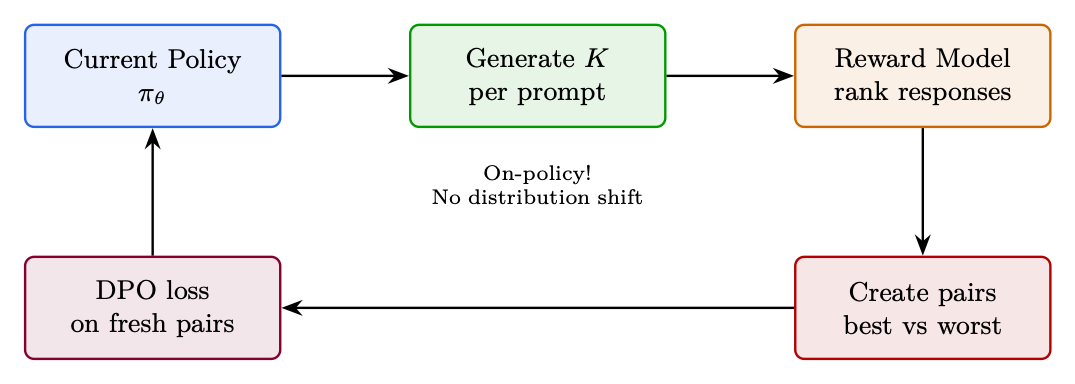
\includegraphics[width=0.85\textwidth]{figures/fig_029_fig29.png}
\caption{GRPO in action: $G{=}5$ responses are sampled for a single math prompt. Three are correct ($r{=}1$), two are wrong ($r{=}0$). The group mean $\mu_G{=}0.6$ acts as the baseline; correct responses receive positive advantage (reinforced), wrong ones receive negative advantage (suppressed).}
\end{figure}

\section{TRL Implementation}
\label{trl-implementation-dup3}

The following shows a minimal working example using HuggingFace TRL.

\begin{lstlisting}[style=pythonstyle]
from trl import GRPOConfig, GRPOTrainer
from transformers import AutoModelForCausalLM, AutoTokenizer

model = AutoModelForCausalLM.from_pretrained("Qwen/Qwen2.5-7B-Instruct",
    torch_dtype=torch.bfloat16, attn_implementation="flash_attention_2")
tokenizer = AutoTokenizer.from_pretrained("Qwen/Qwen2.5-7B-Instruct")

grpo_config = GRPOConfig(
    output_dir="./grpo_output",
    num_generations=8,           # G = group size
    temperature=1.0,             # High temp for diversity within group
    max_completion_length=2048,  # Max response length
    beta=0.04,                   # KL penalty coefficient
    learning_rate=1e-6,
    per_device_train_batch_size=2,  # Prompts per device (x8 gens = 16 responses)
    gradient_accumulation_steps=8,
    num_train_epochs=2,
    bf16=True,
    gradient_checkpointing=True,
    max_grad_norm=0.5,
    logging_steps=10,
    # vLLM generation for speed (critical for GRPO due to 8x generation)
    use_vllm=True,
    vllm_gpu_memory_utilization=0.7,
)

# Reward function: binary correctness for math
def reward_fn(completions, prompts, **kwargs):
    """Return list of floats: 1.0 if correct, 0.0 if wrong."""
    rewards = []
    for completion, prompt in zip(completions, prompts):
        answer = extract_answer(completion)
        expected = get_ground_truth(prompt)
        rewards.append(1.0 if answer == expected else 0.0)
    return rewards

# Can combine multiple reward functions!
def format_reward_fn(completions, **kwargs):
    """Bonus for using proper LaTeX formatting."""
    return [0.5 if "\\boxed{" in c else 0.0 for c in completions]

trainer = GRPOTrainer(
    model=model,
    args=grpo_config,
    reward_funcs=[reward_fn, format_reward_fn],  # Multi-objective!
    train_dataset=math_dataset,
    tokenizer=tokenizer,
)
trainer.train()
\end{lstlisting}

\section{Group Size Analysis}
\label{group-size-analysis}

\begin{tabular}{@{}lp{3.5cm}p{3.5cm}p{6cm}@{}}
\toprule
$G$ & \textbf{Signal Quality} & \textbf{Compute} & \textbf{When to Use} \\
\midrule
2 & Very noisy (coin flip) & Low & Never recommended --- too noisy for stable learning \\
4 & Moderate & Moderate & Quick experiments, easy tasks (pass rate $>$ 50\%) \\
8 & Good (standard) & High & Default. Good balance for most tasks \\
16 & Excellent & Very high & Hard tasks (pass rate $<$ 20\%), need many attempts to get positives \\
32 & Near-perfect & Extreme & Only if you have massive compute and very hard task \\
\bottomrule
\end{tabular}

\begin{keybox}[Critical: Group Must Contain Both Successes and Failures]
If all $G$ responses are correct ($r_i = 1 \;\forall i$): all advantages = 0, no learning signal!\\

If all wrong: same problem. The prompt’s difficulty must match model’s capability.\\

\textbf{Goldilocks rule}: Filter prompts to 20--80\% pass rate for current model. Re-filter every 500 steps as model improves.
\end{keybox}

\section{GRPO Variants and Extensions}
\label{grpo-variants-and-extensions}

\subsection{Diversity in GRPO Groups}
\label{diversity-in-grpo-groups}

\begin{intuitionbox}[Mode Collapse in RL Training]
Without diversity pressure, RL-trained LLMs collapse to a narrow set of high-reward responses:

\begin{itemize}
  \item The model learns one ``template'' answer for each question type
  \item Entropy drops rapidly; the model becomes deterministic
  \item Reward hacking becomes easier (narrow outputs are easier to exploit)
  \item Generalization suffers: the model memorizes reward patterns, not reasoning
\end{itemize}

The KL penalty $\beta D_\text{KL}[\pi_\theta \| \pi_\text{ref}]$ is the primary diversity mechanism, but it’s not sufficient alone.
\end{intuitionbox}

\begin{keybox}[GRPO Group Diversity]
GRPO generates $N$ responses per prompt and uses within-group ranking. Diversity within the group is critical:

\begin{itemize}
  \item \textbf{High temperature} ($\tau=0.8$--$1.0$): Ensures varied responses for meaningful comparison
  \item \textbf{Large $N$} (8--16): More samples = more likely to include both good and bad approaches
  \item \textbf{DAPO’s ``No Repeat'' penalty}: Rejects duplicate responses within a group to force exploration
  \item If all $N$ responses are identical: advantage is zero, no learning signal
  \item If responses are too diverse (random): reward signal is noisy, slow learning
\end{itemize}

\textbf{Sweet spot}: Temperature that gives distinct approaches while staying on-topic.
\end{keybox}

\begin{table}[ht!]
\centering
\caption{Diversity-promoting methods for RL training.}
\begin{tabular}{@{}lp{11cm}@{}}
\toprule
\textbf{Method} & \textbf{How It Promotes Diversity} \\
\midrule
Entropy bonus & Add $\alpha H(\pi_\theta)$ to the reward. Directly penalizes low-entropy (deterministic) policies. \\
KL penalty & $-\beta D_\text{KL}[\pi_\theta \| \pi_\text{ref}]$ prevents collapse toward a single mode. \\
Rejection sampling & Generate many candidates, keep top-$k$ by reward. Naturally selects for diverse high-quality responses. \\
Best-of-N & At inference: generate $N$ responses, score all, return the best. Diversity comes from sampling. \\
DPO with diverse pairs & Train on pairs where chosen/rejected differ in \emph{approach}, not just quality. \\
Multi-reward & Use multiple reward models (safety, helpfulness, code quality). Prevents collapsing to one dimension. \\
\bottomrule
\end{tabular}
\end{table}

\begin{warningbox}[Diversity vs. Quality Tradeoff]
More diversity is not always better:

\begin{itemize}
  \item Too much diversity (high entropy) = random, unhelpful responses
  \item Too little diversity (low entropy) = repetitive, reward-hacked responses
  \item \textbf{Monitor}: Track response entropy, unique n-gram ratio, and reward distribution width during training. If all three are dropping simultaneously, you have a collapse problem.
\end{itemize}
\end{warningbox}

\subsubsection{Verbalized Sampling for RL Data Collection}
\label{verbalized-sampling-for-rl-data-collection}

Post-training alignment (RLHF, DPO) often reduces output diversity due to \emph{typicality bias}: human annotators systematically prefer familiar, ``typical'' text over novel alternatives. This mode collapse is a data-level phenomenon, not purely algorithmic.

Verbalized Sampling (VS)~\cite{zhang2025verbalized} is a training-free prompting strategy that circumvents this collapse by asking the model to \textbf{explicitly verbalize a probability distribution} over multiple responses in a single generation.

\begin{keybox}[Verbalized Sampling – Core Idea]
Instead of sampling a single response (which collapses to the mode), prompt the model to output \emph{multiple candidate responses along with their probabilities}:

\texttt{‘‘Generate 5 jokes about coffee and their corresponding probabilities.’’}

The model produces a list like:

\begin{enumerate}
  \item Joke A (probability: 0.35)
  \item Joke B (probability: 0.25)
  \item Joke C (probability: 0.20)
  \item Joke D (probability: 0.12)
  \item Joke E (probability: 0.08)
\end{enumerate}

Then sample from this verbalized distribution. Because the model explicitly represents the full distribution (not just the argmax), lower-probability but creative/diverse responses become accessible.
\end{keybox}

\begin{lstlisting}[style=pythonstyle]
# Verbalized Sampling: prompt model to output distribution
def verbalized_sample(model, tokenizer, task, n=5):
    prompt = (
        f"{task}\n\n"
        f"Generate {n} different responses and assign a probability "
        f"to each (probabilities should sum to 1.0). "
        f"Format: [response] (probability: X.XX)"
    )
    output = model.generate(
        tokenizer(prompt, return_tensors="pt").input_ids,
        max_new_tokens=1024,
        temperature=0.7,
        do_sample=True,
    )
    # Parse responses and probabilities from output
    responses, probs = parse_verbalized_distribution(
        tokenizer.decode(output[0])
    )
    # Sample from the verbalized distribution
    import random
    chosen = random.choices(responses, weights=probs, k=1)[0]
    return chosen
\end{lstlisting}

\begin{intuitionbox}[Why Verbalized Sampling Works]
\begin{itemize}
  \item \textbf{Bypasses mode collapse}: Standard sampling from aligned models heavily concentrates on one or two ``safe'' responses. VS forces the model to articulate alternatives it \emph{knows} but wouldn’t normally surface.
  \item \textbf{Diversity is semantic}: Unlike temperature scaling (lexical noise), VS produces genuinely different approaches---the model reasons about distinct options.
  \item \textbf{Scales with capability}: More capable models produce better-calibrated verbalized distributions---they benefit \emph{more} from VS (1.6--2.1$\times$ diversity gain in creative writing).
  \item \textbf{Training-free}: No fine-tuning or modified decoding; works with any instruction-following model at inference time.
  \item \textbf{For GRPO}: Use VS to generate the $G$ response candidates per prompt---ensures the group contains semantically diverse approaches rather than surface-level variations.
\end{itemize}
\end{intuitionbox}

Before diving into the extensions, let us briefly recap the base GRPO algorithm established in the previous sections. The core mechanism---sampling a group of completions, normalizing their rewards, and applying a clipped policy gradient---is elegant in its simplicity. However, practitioners quickly discovered specific failure modes: pretraining bias diluting gradients (Dr.~GRPO), symmetric clipping limiting exploration (DAPO), wasteful large group sizes (2-GRPO), and reward-scale imbalance in multi-objective settings (GDPO). The following sections address each of these in turn.

\begin{keybox}[GRPO Baseline Recap]
Given a prompt $q$, sample $G$ completions $\{o_1,\dots,o_G\}$ from the current policy $\pi_\theta$. Compute rewards $\{r_1,\dots,r_G\}$ and normalise: 
\[
\hat{A}_i = \frac{r_i - \mu_r}{\sigma_r + \epsilon}, \qquad
  \mu_r = \frac{1}{G}\sum_{i=1}^G r_i, \quad
  \sigma_r = \sqrt{\frac{1}{G}\sum_{i=1}^G (r_i-\mu_r)^2}.
\]
 The clipped surrogate loss (per token) is: 
\[
\mathcal{L}_{\text{GRPO}} = -\frac{1}{G}\sum_{i=1}^G \frac{1}{|o_i|}
    \sum_{t=1}^{|o_i|}
    \min\!\Bigl(
      \rho_{i,t}\,\hat{A}_i,\;
      \mathrm{clip}(\rho_{i,t},1{-}\epsilon,1{+}\epsilon)\,\hat{A}_i
    \Bigr),
\]
 where $\rho_{i,t} = \pi_\theta(o_{i,t}|q,o_{i,<t})\,/\,\pi_{\text{old}}(o_{i,t}|q,o_{i,<t})$.
\end{keybox}

\subsection{DAPO -- Dynamic Adaptive Policy Optimization}
\label{sec:dapo}

\begin{intuitionbox}[Why DAPO?]
Base GRPO uses \emph{symmetric} clipping: the policy is equally constrained whether it wants to increase or decrease the probability of a token. But exploration and exploitation have different risk profiles. Increasing the probability of a good token is generally safe; suppressing a token that happened to appear in a bad completion can be catastrophically wrong if the token itself is neutral. DAPO~\cite{yu2025dapo} introduces five targeted fixes that together substantially improve training stability and final performance.
\end{intuitionbox}

\subsubsection*{Component 1 -- Asymmetric Clipping (Clip-Higher)}
\label{component-1-asymmetric-clipping-clip-higher}

Standard PPO/GRPO clips the importance ratio symmetrically at $[1-\epsilon, 1+\epsilon]$. DAPO replaces this with an asymmetric band:

\[
\boxed{
    \mathrm{clip}_{\text{DAPO}}(\rho, A) =
    \begin{cases}
      \mathrm{clip}(\rho,\, 1-\epsilon,\, 1+\epsilon_{\text{high}}) & \text{if } A > 0 \\
      \mathrm{clip}(\rho,\, 1-\epsilon,\, 1+\epsilon) & \text{if } A \le 0
    \end{cases}
  }
\]

where $\epsilon_{\text{high}} > \epsilon$ (typical values: $\epsilon=0.2$, $\epsilon_{\text{high}}=0.28$). When the advantage is positive the policy is allowed to move further toward the good token; when the advantage is negative the usual conservative clipping applies to avoid over-suppression.

\subsubsection*{Component 2 -- Token-Level Loss Aggregation}
\label{component-2-token-level-loss-aggregation}

Base GRPO divides the loss by the \emph{number of sequences} $G$. DAPO divides by the \emph{total number of tokens} across all sequences:

\[
\mathcal{L}_{\text{token}} =
    -\frac{1}{\sum_{i=1}^G |o_i|}
    \sum_{i=1}^G \sum_{t=1}^{|o_i|}
    \min\!\bigl(\rho_{i,t}\hat{A}_i,\;
                \mathrm{clip}_{\text{DAPO}}(\rho_{i,t},\hat{A}_i)\,\hat{A}_i\bigr).
\]

This prevents long completions from dominating the gradient signal simply because they contain more tokens.

\subsubsection*{Component 3 -- Overlong Filtering}
\label{component-3-overlong-filtering}

When a completion is truncated (no EOS token within the maximum length budget), it provides \emph{misleading} signal: the model is penalised for tokens that were generated correctly but happened to appear before the truncation boundary. DAPO masks these completions entirely:

\[
m_i = \mathbf{1}[\text{EOS} \in o_i], \qquad
  \mathcal{L}_{\text{filtered}} =
    -\frac{\sum_{i=1}^G m_i \sum_t (\cdots)}{\sum_{i=1}^G m_i |o_i|}.
\]

\subsubsection*{Component 4 -- Soft Overlong Punishment}
\label{component-4-soft-overlong-punishment}

Rather than a hard mask, a softer variant applies a length penalty that grows smoothly as completions approach the maximum length $L_{\max}$:

\[
r_i \leftarrow r_i - \lambda \cdot \max\!\left(0,\, \frac{|o_i| - L_{\text{cache}}}{L_{\max} - L_{\text{cache}}}\right),
\]

where $L_{\text{cache}}$ is a ``safe'' length threshold.

\subsubsection*{Component 5 -- Dynamic Sampling}
\label{component-5-dynamic-sampling}

DAPO re-samples prompts whose entire group of completions receives the same reward (all correct or all incorrect), because such groups contribute zero gradient after normalisation. This keeps the effective batch size stable throughout training.

\begin{examplebox}[DAPO in TRL]
\begin{lstlisting}[style=pythonstyle]
from trl import GRPOConfig, GRPOTrainer

config = GRPOConfig(
    # Asymmetric clipping
    epsilon=0.2,
    epsilon_high=0.28,          # Clip-Higher
    # Token-level loss
    loss_type="dapo",           # enables token-level aggregation
    # Overlong filtering
    mask_truncated_completions=True,
    # Generation budget
    max_completion_length=1024,
    num_generations=8,
    # Note: DAPO loss internally handles zero-variance group filtering
)

trainer = GRPOTrainer(
    model=model,
    reward_funcs=[reward_fn],
    args=config,
    train_dataset=dataset,
)
trainer.train()
\end{lstlisting}
\end{examplebox}

\begin{keybox}[When to Use DAPO]
\begin{itemize}
  \item Long-form reasoning tasks where completions frequently hit the length limit.
  \item Any setting where you observe reward variance collapsing mid-training.
  \item When base GRPO shows instability (loss spikes, entropy collapse).
  \item Recommended as a \emph{drop-in improvement} over base GRPO for most tasks.
\end{itemize}
\end{keybox}

\subsection{GSPO -- Group Sequence Policy Optimization}
\label{sec:gspo}

\begin{intuitionbox}[The Off-Policy Problem]
GRPO clips importance ratios \emph{per token}. But a sequence of 500 tokens can have a product of per-token ratios that is astronomically large or small, even if each individual ratio is within $[1-\epsilon, 1+\epsilon]$. When training for multiple gradient steps on the same batch (off-policy), this mismatch grows rapidly and the clipping bound becomes meaningless at the sequence level.
\end{intuitionbox}

GSPO~\cite{chen2025gspo} defines a \emph{sequence-level} importance weight as the geometric mean of per-token ratios, which equals the $|o_i|$-th root of the full sequence probability ratio:

\[
\boxed{
    s_i(\theta) = \left(\frac{\pi_\theta(o_i \mid q)}{\pi_{\text{old}}(o_i \mid q)}\right)^{1/|o_i|}
    = \exp\!\left(\frac{1}{|o_i|}\sum_{t=1}^{|o_i|} \log \frac{\pi_\theta(o_{i,t}|q,o_{i,<t})}{\pi_{\text{old}}(o_{i,t}|q,o_{i,<t})}\right).
  }
\]

This is the \emph{length-normalised} sequence probability ratio. The GSPO loss clips this single scalar per sequence:

\[
\mathcal{L}_{\text{GSPO}} = -\frac{1}{G}\sum_{i=1}^G
    \min\!\Bigl(s_i(\theta)\,\hat{A}_i,\;
               \mathrm{clip}(s_i(\theta),1{-}\epsilon,1{+}\epsilon)\,\hat{A}_i\Bigr).
\]

\begin{keybox}[GSPO vs GRPO Clipping]
\begin{itemize}
  \item \textbf{GRPO}: clips each of the $|o_i|$ per-token ratios independently. A sequence can have all ratios within bounds yet have a product ratio of $10^{50}$.
  \item \textbf{GSPO}: clips the geometric mean once per sequence. Guarantees the \emph{sequence-level} policy shift is bounded.
  \item GSPO is theoretically correct for off-policy IS; GRPO is an approximation.
\end{itemize}
\end{keybox}

\begin{examplebox}[GSPO in TRL]
\begin{lstlisting}[style=pythonstyle]
from trl import GRPOConfig, GRPOTrainer

config = GRPOConfig(
    # Sequence-level importance sampling
    importance_sampling_level="sequence",   # GSPO mode
    # Off-policy: reuse each batch for multiple gradient steps
    steps_per_generation=4,
    num_generations=8,
    epsilon=0.2,
)

trainer = GRPOTrainer(
    model=model,
    reward_funcs=[reward_fn],
    args=config,
    train_dataset=dataset,
)
\end{lstlisting}
\end{examplebox}

\begin{warningbox}[When to Use GSPO]
GSPO is most beneficial when \texttt{steps\_per\_generation > 1} (off-policy training). For purely on-policy training ($\text{steps\_per\_generation}=1$) the difference from GRPO is negligible. Off-policy training can dramatically reduce generation cost (the most expensive step), making GSPO + off-policy a strong efficiency choice.
\end{warningbox}

\subsection{Dr.~GRPO -- Debiased Reward GRPO}
\label{sec:dr-grpo}

\begin{intuitionbox}[The Pretraining Bias Problem]
Standard GRPO normalises advantages within a group, but the \emph{pretraining distribution} introduces a systematic bias: tokens that are common in pretraining data receive large gradients even when they carry no task-relevant information. Dr.~GRPO~\cite{liu2024drgrpo} identifies and corrects this bias, focusing gradient signal on \emph{informative} tokens.
\end{intuitionbox}

Dr.~GRPO modifies the per-token gradient weight to account for the token’s marginal contribution to the reward signal. Tokens that the model already assigns high probability to (regardless of the reward) are down-weighted:

\[
w_{i,t} = \hat{A}_i \cdot \bigl(1 - \pi_{\text{ref}}(o_{i,t}|q,o_{i,<t})\bigr),
\]

where $\pi_{\text{ref}}$ is the reference (pretrained) model. This is a form of \emph{token efficiency}: the gradient is concentrated on tokens where the policy genuinely needs to change.

\begin{examplebox}[Dr. GRPO in TRL]
\begin{lstlisting}[style=pythonstyle]
from trl import GRPOConfig, GRPOTrainer

config = GRPOConfig(
    loss_type="dr_grpo",
    num_generations=8,
    beta=0.04,   # KL penalty coefficient
)

trainer = GRPOTrainer(
    model=model,
    ref_model=ref_model,   # required for token weighting
    reward_funcs=[reward_fn],
    args=config,
    train_dataset=dataset,
)
\end{lstlisting}
\end{examplebox}

\begin{keybox}[When to Use Dr. GRPO]
\begin{itemize}
  \item When training on tasks with a large vocabulary mismatch between pretraining and RL.
  \item When you observe that common filler tokens dominate the gradient.
  \item Pairs well with a reference model that is close to the initial policy.
\end{itemize}
\end{keybox}

\subsection{2-GRPO -- Minimal Two-Rollout GRPO}
\label{sec:2grpo}

\begin{intuitionbox}[``It Takes Two'' Insight]
The ``It Takes Two'' paper~\cite{xu2025twograpo} demonstrates empirically and theoretically that GRPO with $G=2$ (just two completions per prompt) matches or exceeds GRPO with $G=16$ on most reasoning benchmarks. This is surprising -- why would fewer samples be sufficient?
\end{intuitionbox}

The key insight is that GRPO’s effectiveness does \emph{not} primarily come from accurate advantage estimation (which requires large $G$). Instead, it comes from an implicit \emph{contrastive objective} that is structurally similar to DPO:

\[
\mathcal{L}_{\text{2-GRPO}} \approx
  -\mathbb{E}_{(o^+, o^-) \sim \pi_\theta}\!\left[
    \log \sigma\!\left(
      \beta \log \frac{\pi_\theta(o^+|q)}{\pi_{\text{old}}(o^+|q)}
      - \beta \log \frac{\pi_\theta(o^-|q)}{\pi_{\text{old}}(o^-|q)}
    \right)
  \right],
\]

where $o^+$ is the higher-reward completion and $o^-$ the lower-reward one. With $G=2$, this contrastive structure is explicit. With $G=16$, the same signal is present but diluted by redundant pairs.

\begin{keybox}[Compute Savings from 2-GRPO]
\begin{itemize}
  \item $G=2$ vs $G=16$: \textbf{8$\times$ less generation compute}.
  \item Generation is typically the bottleneck (60--80\% of wall-clock time).
  \item Total training speedup: approximately 4--6$\times$ end-to-end.
  \item No accuracy loss on GSM8K, MATH, and code benchmarks.
\end{itemize}
\end{keybox}

\begin{examplebox}[2-GRPO in TRL]
\begin{lstlisting}[style=pythonstyle]
from trl import GRPOConfig, GRPOTrainer

config = GRPOConfig(
    num_generations=2,      # The key change -- just two rollouts
    loss_type="grpo",       # Standard GRPO loss is fine
    epsilon=0.2,
    # With G=2, batch size must be at least 2 * num_prompts_per_step
    per_device_train_batch_size=2,
)

trainer = GRPOTrainer(
    model=model,
    reward_funcs=[reward_fn],
    args=config,
    train_dataset=dataset,
)
\end{lstlisting}
\end{examplebox}

\begin{warningbox}[Caveats of 2-GRPO]
With $G=2$, advantage normalisation is over only two values, so the normalised advantages are always $\{+1, -1\}$ (or $\{0, 0\}$ if rewards are equal). This means the gradient magnitude is fixed regardless of the reward gap. For tasks where the \emph{magnitude} of the reward difference matters (e.g., partial credit), larger $G$ may still be beneficial.
\end{warningbox}

\subsection{SAPO -- Soft Adaptive Policy Optimization}
\label{sec:sapo}

\begin{intuitionbox}[The Brittleness of Hard Clipping]
PPO-style clipping creates a discontinuous gradient: the gradient is zero outside the clip band and non-zero inside. This ``cliff edge'' can cause instability near the boundary and makes the trust region sensitive to the choice of $\epsilon$. SAPO~\cite{han2025sapo} replaces the hard clip with a smooth, temperature-controlled gate function.
\end{intuitionbox}

SAPO replaces the $\min(\rho A, \mathrm{clip}(\rho,\cdot)\,A)$ objective with a smooth surrogate:

\[
\boxed{
    \mathcal{L}_{\text{SAPO}}(\rho, A) =
    \begin{cases}
      -A \cdot \sigma\!\left(\dfrac{\rho - 1}{\tau_+}\right) \cdot \rho
        & \text{if } A > 0 \\[8pt]
      -A \cdot \sigma\!\left(\dfrac{1 - \rho}{\tau_-}\right) \cdot \rho
        & \text{if } A \le 0
    \end{cases}
  }
\]

where $\sigma$ is the sigmoid function and $\tau_+, \tau_-$ are asymmetric temperature parameters. A higher temperature produces a softer gate (more exploration); a lower temperature approaches hard clipping.

\begin{keybox}[SAPO Temperature Intuition]
\begin{itemize}
  \item $\tau_+ = 1.0$: moderate gate for positive advantages (allow exploration).
  \item $\tau_- = 1.05$: slightly softer gate for negative advantages (avoid over-suppression).
  \item As $\tau \to 0$: recovers hard PPO clipping.
  \item As $\tau \to \infty$: recovers unclipped policy gradient.
\end{itemize}
\end{keybox}

\begin{examplebox}[SAPO in TRL]
\begin{lstlisting}[style=pythonstyle]
from trl import GRPOConfig, GRPOTrainer

config = GRPOConfig(
    loss_type="sapo",
    sapo_temperature_pos=1.0,    # tau_+ for positive advantages
    sapo_temperature_neg=1.05,   # tau_- for negative advantages
    num_generations=8,
)

trainer = GRPOTrainer(
    model=model,
    reward_funcs=[reward_fn],
    args=config,
    train_dataset=dataset,
)
\end{lstlisting}
\end{examplebox}

\subsection{TIS and MIS -- Truncated and Masked Importance Sampling}
\label{sec:tis-mis}

\begin{warningbox}[The Silent vLLM Probability Mismatch]
When using vLLM for fast generation, the log-probabilities returned by vLLM differ from those computed during the training forward pass~\cite{zhong2025tismis}. This is \emph{not} a bug -- it arises from different CUDA kernels, different floating-point precision, and different attention implementations (e.g., FlashAttention vs PagedAttention). The mismatch silently breaks the on-policy assumption: the ``old policy'' probabilities used to compute importance ratios are wrong, leading to biased gradient estimates.
\end{warningbox}

\subsubsection*{Truncated Importance Sampling (TIS)}
\label{truncated-importance-sampling-tis}

TIS corrects the bias by multiplying the gradient by a truncated correction factor:

\[
\boxed{
    w_{\text{TIS}}(o_i) = \min\!\left(C,\; \frac{\pi_{\text{train}}(o_i|q)}{\pi_{\text{vllm}}(o_i|q)}\right),
  }
\]

where $\pi_{\text{train}}$ is the probability from the training forward pass and $\pi_{\text{vllm}}$ is the probability reported by vLLM. The truncation at $C$ prevents extreme corrections from destabilising training.

\subsubsection*{Masked Importance Sampling (MIS)}
\label{masked-importance-sampling-mis}

MIS takes a harder approach: it zeros out the gradient for any sequence where the correction ratio exceeds a threshold $C$:

\[
w_{\text{MIS}}(o_i) = \mathbf{1}\!\left[\frac{\pi_{\text{train}}(o_i|q)}{\pi_{\text{vllm}}(o_i|q)} \le C\right].
\]

This is more conservative but avoids the risk of large (even truncated) correction weights.

\subsubsection*{Sequence-Level vs Token-Level IS}
\label{sequence-level-vs-token-level-is}

Both TIS and MIS can be applied at the token level or the sequence level:

\begin{itemize}
  \item \textbf{Sequence-level}: compute the ratio as the geometric mean over all tokens (as in GSPO). Theoretically correct but higher variance.
  \item \textbf{Token-level}: compute a separate ratio for each token. Biased (the product of per-token corrections is not the sequence correction) but lower variance.
\end{itemize}

\begin{examplebox}[TIS and MIS in TRL]
\begin{lstlisting}[style=pythonstyle]
from trl import GRPOConfig, GRPOTrainer

# Truncated IS correction for vLLM probability mismatch
config_tis = GRPOConfig(
    use_vllm=True,
    vllm_importance_sampling_correction=True,
    vllm_importance_sampling_mode="sequence_truncate",  # TIS
    vllm_importance_sampling_cap=5.0,                   # C threshold
)

# Masked IS correction
config_mis = GRPOConfig(
    use_vllm=True,
    vllm_importance_sampling_correction=True,
    vllm_importance_sampling_mode="sequence_mask",      # MIS
    vllm_importance_sampling_cap=3.0,
)
\end{lstlisting}
\end{examplebox}

\begin{keybox}[When to Use TIS/MIS]
\begin{itemize}
  \item \textbf{Always} consider enabling when using vLLM for generation.
  \item TIS is preferred when the mismatch is small (same model, different precision).
  \item MIS is preferred when the mismatch is large or unpredictable.
  \item Sequence-level IS is theoretically preferred; token-level is a practical compromise.
\end{itemize}
\end{keybox}

\subsection{VESPO -- Variational Sequence-Level Soft Policy Optimization}
\label{sec:vespo}

\begin{intuitionbox}[Principled Reward Reshaping]
Most GRPO variants modify the clipping mechanism heuristically. VESPO derives a principled reward-reshaping kernel from a variational inference framework, treating policy optimisation as approximate posterior inference. VESPO~\cite{luo2025vespo} derives a resulting kernel that is smooth, asymmetric, and naturally handles staleness in asynchronous or off-policy training.
\end{intuitionbox}

VESPO derives a weighting function $W(\tau)$ for each trajectory $\tau$ from the variational objective. The final gradient weight takes the form:

\[
\boxed{
    g(\tau) = W(\tau)^k \cdot \exp\!\bigl(\lambda(1 - W(\tau))\bigr),
  }
\]

where $W(\tau) = \pi_\theta(\tau)/\pi_{\text{old}}(\tau)$ is the sequence-level importance weight, $k$ controls the sharpness of the weighting, and $\lambda$ controls the exponential decay for stale (low-weight) trajectories. This kernel:

\begin{itemize}
  \item Is smooth everywhere (no discontinuous gradient at clip boundaries).
  \item Naturally down-weights stale trajectories ($W \ll 1$) via the exponential term.
  \item Is asymmetric: high-weight trajectories ($W > 1$) are treated differently from low-weight ones.
\end{itemize}

\begin{examplebox}[VESPO in TRL]
\begin{lstlisting}[style=pythonstyle]
from trl import GRPOConfig, GRPOTrainer

config = GRPOConfig(
    loss_type="vespo",
    vespo_k_pos=2.0,         # sharpness exponent (positive advantages)
    vespo_lambda_pos=3.0,    # staleness decay (positive advantages)
    num_generations=8,
    steps_per_generation=2,  # off-policy; VESPO handles staleness
)

trainer = GRPOTrainer(
    model=model,
    reward_funcs=[reward_fn],
    args=config,
    train_dataset=dataset,
)
\end{lstlisting}
\end{examplebox}

\subsection{DPPO -- Direct Policy Divergence Policy Optimization}
\label{sec:dppo}

\begin{intuitionbox}[The Problem with Ratio Clipping]
PPO’s ratio clipping is a proxy for constraining the KL divergence between old and new policy. But the proxy is imperfect: clipping over-penalises low-probability tokens (where a small absolute change in probability corresponds to a large ratio change) and under-penalises high-probability tokens (where a large absolute change corresponds to a small ratio change). DPPO~\cite{an2025dppo} replaces ratio clipping with \emph{direct divergence estimates}.
\end{intuitionbox}

DPPO computes the trust region constraint directly using either Total Variation (TV) or KL divergence between the old and new policy distributions:

\[
\mathcal{L}_{\text{DPPO}} = -\mathbb{E}\!\left[
    \hat{A} \cdot \pi_\theta(o|q) \cdot \mathbf{1}[D(\pi_\theta \| \pi_{\text{old}}) \le \delta]
  \right],
\]

where $D$ is the chosen divergence measure. In practice, DPPO approximates this with token-level binary or top-$k$ masks:

\begin{itemize}
  \item \textbf{binary\_tv}: mask tokens where $|\pi_\theta - \pi_{\text{old}}| > \delta$.
  \item \textbf{binary\_kl}: mask tokens where $\pi_\theta \log(\pi_\theta/\pi_{\text{old}}) > \delta$.
  \item \textbf{topk\_tv}: keep only the top-$k$ tokens by TV contribution.
  \item \textbf{topk\_kl}: keep only the top-$k$ tokens by KL contribution.
\end{itemize}

\begin{examplebox}[DPPO – Conceptual Implementation]
DPPO is not yet available as a built-in TRL trainer. A custom implementation would use GRPOTrainer with a modified loss that clips based on distributional divergence (TV or KL) rather than the standard probability ratio:

\begin{lstlisting}[style=pythonstyle]
# Pseudocode: DPPO requires a custom trainer subclass
from trl import GRPOConfig, GRPOTrainer

config = GRPOConfig(
    num_generations=8,
    beta=0.04,
)
# Override the loss computation to use distributional clipping:
# clip when TV(pi_new || pi_old) > delta, rather than when
# pi_new/pi_old exceeds [1-eps, 1+eps]
\end{lstlisting}
\end{examplebox}

\begin{warningbox}[DPPO is Research-Stage]
DPPO is a recent research contribution and is not yet integrated into mainstream RL libraries. It is most useful when you observe that standard ratio clipping is failing (e.g., on tasks with highly skewed token probability distributions).
\end{warningbox}

\subsection{ScaleRL and CISPO}
\label{sec:scalerl-cispo}

\begin{intuitionbox}[Scaling Laws for RL]
The ScaleRL paper~\cite{luo2025scalerl} conducts a systematic study of what makes RL training for LLMs scale effectively. The key finding is that two modifications -- batch-level reward scaling and DAPO-style token-level loss -- together unlock strong performance at scale, while neither alone is sufficient. CISPO (Clipped IS Policy Optimization) is the resulting algorithm.
\end{intuitionbox}

\subsubsection*{Batch-Level Reward Scaling}
\label{batch-level-reward-scaling}

Standard GRPO normalises rewards within a group of $G$ completions for a single prompt. CISPO normalises rewards across the \emph{entire batch}:

\[
\hat{A}_i = \frac{r_i - \mu_{\text{batch}}}{\sigma_{\text{batch}} + \epsilon},
\]

where $\mu_{\text{batch}}$ and $\sigma_{\text{batch}}$ are computed over all rewards in the current training batch. This provides a more stable baseline and prevents any single prompt from dominating the gradient.

\subsubsection*{CISPO Loss}
\label{cispo-loss}

CISPO combines batch-level scaling with DAPO’s token-level loss aggregation and asymmetric clipping:

\[
\mathcal{L}_{\text{CISPO}} =
    -\frac{1}{\sum_{i,t} m_{i,t}}
    \sum_{i=1}^G \sum_{t=1}^{|o_i|} m_{i,t} \cdot
    \min\!\bigl(\rho_{i,t}\hat{A}_i,\;
               \mathrm{clip}_{\text{DAPO}}(\rho_{i,t},\hat{A}_i)\,\hat{A}_i\bigr),
\]

where $m_{i,t}$ is the overlong-filtering mask.

\begin{examplebox}[CISPO in TRL]
\begin{lstlisting}[style=pythonstyle]
from trl import GRPOConfig, GRPOTrainer

config = GRPOConfig(
    loss_type="cispo",
    scale_rewards="batch",          # batch-level reward normalisation
    mask_truncated_completions=True,
    epsilon=0.2,
    epsilon_high=5.0,               # epsilon_max for CISPO (ScaleRL paper)
    num_generations=8,
)

trainer = GRPOTrainer(
    model=model,
    reward_funcs=[reward_fn],
    args=config,
    train_dataset=dataset,
)
\end{lstlisting}
\end{examplebox}

\begin{keybox}[ScaleRL Key Findings]
\begin{enumerate}
  \item Batch-level reward scaling alone: modest improvement.
  \item Token-level loss alone: modest improvement.
  \item Both together: \textbf{synergistic} -- significantly better than either alone.
  \item Larger batch sizes benefit more from batch-level scaling.
  \item CISPO is the recommended default for large-scale RL training.
\end{enumerate}
\end{keybox}

\subsection{GDPO -- Group Reward-Decoupled Policy Optimization}
\label{sec:gdpo}

\begin{intuitionbox}[The Multi-Reward Collapse Problem]
In multi-objective RL (e.g., optimising for both correctness and format), standard GRPO normalises the \emph{combined} reward. If one reward has much higher variance than another, it dominates the normalised advantage, effectively ignoring the other reward. This is \emph{advantage collapse}: the low-variance reward contributes near-zero gradient. GDPO~\cite{zhong2025gdpo} normalises each reward \emph{independently} before aggregating.
\end{intuitionbox}

The core mechanism normalises each reward \emph{independently} before aggregating:

\[
\boxed{
    \hat{A}_n^{(i)} = \frac{r_n^{(i)} - \mu_n}{\sigma_n + \epsilon}, \qquad
    \hat{A}^{(i)} = \sum_{n=1}^N w_n \hat{A}_n^{(i)},
  }
\]

where $r_n^{(i)}$ is the $n$-th reward for completion $i$, $\mu_n$ and $\sigma_n$ are the mean and standard deviation of reward $n$ within the group, and $w_n$ are user-specified weights.

\begin{keybox}[GDPO vs Standard Multi-Reward GRPO]
\begin{itemize}
  \item \textbf{Standard}: $\hat{A}^{(i)} = \frac{\sum_n w_n r_n^{(i)} - \mu_{\text{combined}}}{\sigma_{\text{combined}}}$. High-variance rewards dominate.
  \item \textbf{GDPO}: normalise each reward separately, then combine. Each reward contributes proportionally to its weight $w_n$.
  \item GDPO is essential when rewards have very different scales or variances.
\end{itemize}
\end{keybox}

\begin{examplebox}[GDPO in TRL]
\begin{lstlisting}[style=pythonstyle]
from trl import GRPOConfig, GRPOTrainer

config = GRPOConfig(
    multi_objective_aggregation="normalize_then_sum",
    reward_weights=[1.0, 0.5],   # weights for [correctness, format]
    num_generations=8,
)

def correctness_reward(completions, **kwargs):
    return [1.0 if is_correct(c) else 0.0 for c in completions]

def format_reward(completions, **kwargs):
    return [0.1 if has_good_format(c) else 0.0 for c in completions]

trainer = GRPOTrainer(
    model=model,
    reward_funcs=[correctness_reward, format_reward],
    args=config,
    train_dataset=dataset,
)
\end{lstlisting}
\end{examplebox}

\subsection{GOPO -- Group Ordinal Policy Optimization}
\label{gopo-group-ordinal-policy-optimization}

GOPO~\cite{choi2025gopo} starts from a simple observation: reward models are trained with pairwise comparisons (``is A better than B?''), so only the \textbf{rank order} of their outputs is trustworthy---the raw numeric scores carry no inherent meaning. Yet GRPO feeds those raw magnitudes directly into the advantage calculation. For tasks with non-verifiable rewards---summarization, open-ended chat, instruction following---this mismatch introduces noise, because a gap of 0.6 reward points might reflect genuine quality in one region of the output space and mean nothing in another.

\textbf{Key Insight}: Discard reward magnitudes entirely. Use only the \textbf{ordinal ranking} of rewards within a group.

\textbf{Algorithm}: Given a group of $N$ responses $\{o_1, \ldots, o_N\}$ with rewards $\{r_1, \ldots, r_N\}$:

\begin{enumerate}
  \item Rank responses by reward: assign rank $\text{rank}(o_i) \in \{1, \ldots, N\}$ (1 = worst, $N$ = best).
  \item Replace raw advantages with rank-based scores: 
\begin{equation}
\boxed{\hat{A}_i^{\text{GOPO}} = f\!\left(\frac{\text{rank}(o_i)}{N}\right)}
\end{equation}
 where $f$ is a monotonic transformation (e.g., linear mapping to $[-1, 1]$ or quantile normalization).
  \item Apply PPO-style clipped objective using rank-based advantages.
\end{enumerate}

\textbf{Comparison with GRPO}:

\begin{tabular}{@{}lp{5cm}p{8cm}@{}}
\toprule
\textbf{Aspect} & \textbf{GRPO} & \textbf{GOPO} \\
\midrule
Advantage signal & $\hat{A}_i = (r_i - \mu)/\sigma$ (uses magnitudes) & $\hat{A}_i = f(\text{rank}_i / N)$ (uses ordinal rank only) \\
Sensitivity to reward scale & High --- miscalibrated RM scores distort advantages & None --- invariant to monotonic reward transformations \\
Best for & Verifiable rewards (binary, well-calibrated) & Non-verifiable rewards (RM-based, noisy magnitudes) \\
\bottomrule
\end{tabular}

\textbf{Empirical gains} (over GRPO on non-verifiable tasks):

\begin{itemize}
  \item Reward curves (both training and held-out) sit above GRPO throughout optimization
  \item Win-rates judged by a separate LLM evaluator improve at most training checkpoints
  \item Convergence is markedly faster---matching GRPO’s final quality with fewer gradient steps
  \item The advantage grows as the reward model becomes noisier or more poorly calibrated
\end{itemize}

\begin{intuitionbox}[When to Use GOPO vs. GRPO]
\begin{itemize}
  \item \textbf{Use GRPO}: When rewards are verifiable and exact (math correctness, code tests pass/fail, binary signals). Magnitudes carry meaningful information.
  \item \textbf{Use GOPO}: When rewards come from a learned reward model on subjective tasks (helpfulness, style, safety). The RM’s relative ordering is trustworthy but its absolute scores are arbitrary.
\end{itemize}
\end{intuitionbox}

\chapter{Preference Optimization Variants}
\label{ch:po-variants}

This chapter covers the family of methods that extend or replace DPO with different objectives, data assumptions, or architectural trade-offs. Each addresses a specific limitation of standard offline DPO: distribution shift (Online DPO), the need for paired data (KTO), overfitting to noisy labels (IPO), reference model memory cost (ORPO), or training complexity (Best-of-N).

\section{Online DPO}
\label{sec:online-dpo}

\subsection{Motivation}
\label{motivation-dup3}

Standard DPO’s primary limitation: the preference data was generated by a \emph{different} model (often an older checkpoint or even a different model family). As training progresses, the policy generates text that looks nothing like the training pairs $\rightarrow$ the loss is optimizing on an irrelevant distribution.

\textbf{Online DPO solution}~\cite{guo2024direct}: Generate fresh preference pairs from the \emph{current} policy at every step, judge them with a reward model, then apply the DPO loss.

\subsection{Algorithm}
\label{algorithm-dup2}

\begin{enumerate}
  \item Generate $K$ responses per prompt from current $\pi_\theta$
  \item Score all responses with reward model $r_\phi$
  \item Create pairs: highest-scoring = chosen, lowest-scoring = rejected
  \item Apply DPO loss on these fresh pairs
  \item Repeat (new generation every step)
\end{enumerate}

\begin{intuitionbox}[Online DPO = Best of Both Worlds]
\begin{itemize}
  \item From DPO: simple supervised loss, no value function, no GAE, stable optimization
  \item From PPO: on-policy data, self-improvement beyond dataset, no distribution shift
  \item Key difference from GRPO: uses DPO loss (pair-based) instead of PPO loss (per-sample advantage)
\end{itemize}

\textbf{Trade-off}: Needs a reward model (DPO doesn’t), but no value head (PPO does). Middle ground complexity.
\end{intuitionbox}


\subsection{TRL Implementation}
\label{trl-implementation-dup4}

The following shows a minimal working example using HuggingFace TRL.

\begin{lstlisting}[style=pythonstyle]
from trl import OnlineDPOConfig, OnlineDPOTrainer
from transformers import AutoModelForCausalLM, AutoModelForSequenceClassification

model = AutoModelForCausalLM.from_pretrained("meta-llama/Llama-3.1-8B-Instruct",
    torch_dtype=torch.bfloat16)
reward_model = AutoModelForSequenceClassification.from_pretrained(
    "RLHFlow/ArmoRM-Llama3-8B-v0.1", torch_dtype=torch.bfloat16)

online_dpo_config = OnlineDPOConfig(
    output_dir="./online_dpo_output",
    learning_rate=5e-7,
    beta=0.1,                    # DPO beta (same meaning as standard DPO)
    num_generations=4,           # K responses per prompt
    per_device_train_batch_size=4,
    gradient_accumulation_steps=4,
    max_new_tokens=512,
    temperature=0.7,
    bf16=True,
    num_train_epochs=1,
    logging_steps=10,
)

trainer = OnlineDPOTrainer(
    model=model,
    reward_model=reward_model,
    args=online_dpo_config,
    train_dataset=prompt_dataset,
    tokenizer=tokenizer,
)
trainer.train()
\end{lstlisting}

\subsection{Online DPO vs Offline DPO vs PPO}
\label{online-dpo-vs-offline-dpo-vs-ppo}

\begin{tabular}{@{}llp{4.5cm}lp{4.5cm}@{}}
\toprule
 & \textbf{Data} & \textbf{Models} & \textbf{Loss} & \textbf{Best For} \\
\midrule
Offline DPO & Static pairs & 2 (policy + reference) & DPO & Quick alignment, limited compute \\
Online DPO & Fresh from $\pi_\theta$ & 3 (policy + reference + reward model) & DPO & When DPO plateaus, need exploration \\
PPO & Fresh from $\pi_\theta$ & 4 (policy + reference + reward model + value head) & PPO clip & Max quality, complex reasoning \\
\bottomrule
\end{tabular}

\section{KTO --- Kahneman-Tversky Optimization}
\label{sec:kto}

\subsection{Motivation}
\label{motivation-1}

DPO requires \emph{paired} preferences: for the same prompt, you need both a good and bad response. In practice, most feedback is \emph{unpaired}: users give thumbs up/down on individual responses, with no matched pair.

\textbf{KTO’s insight}~\cite{ethayarajh2024kto}: Use prospect theory (from behavioral economics). Humans feel losses more strongly than gains. A ``thumbs down'' should produce a stronger gradient than a ``thumbs up.''

\subsection{Loss Function}
\label{loss-function}

\begin{equation}
\boxed{\mathcal{L}_\text{KTO} = \mathbb{E}_{y_w}\left[\lambda_w (1 - v(x, y_w))\right] + \mathbb{E}_{y_l}\left[\lambda_l \cdot v(x, y_l)\right]}
\end{equation}
 where $v(x,y) = \sigma\left(\beta \log\frac{\pi_\theta(y|x)}{\pi_\text{ref}(y|x)} - z_\text{ref}\right)$, and $z_\text{ref}$ is the expected KL divergence (a running baseline).

\begin{intuitionbox}[KTO Intuition via Prospect Theory]
\textbf{Desirable responses} ($y_w$): The model gets ``utility'' from increasing their probability. But with diminishing returns --- once it’s already quite likely, don’t push harder.

\textbf{Undesirable responses} ($y_l$): Loss aversion means the penalty for generating bad text is weighted more strongly than the reward for good text. Default: $\lambda_l = 1.0$, $\lambda_w = 1.0$, but you can set $\lambda_l > \lambda_w$.

\textbf{Key advantage}: Each training example is independent! No need to find matched pairs. Can use thumbs-up/down data directly.
\end{intuitionbox}

\begin{examplebox}[KTO Data Format]
Unlike DPO which needs: \verb|{"prompt": ..., "chosen": ..., "rejected": ...}|

KTO only needs: \verb|{"prompt": ..., "completion": ..., "label": true/false}|

This means you can use:

\begin{itemize}
  \item Thumbs up/down from production traffic
  \item Upvotes/downvotes from forums
  \item Human ratings binarized (4--5 stars = good, 1--2 = bad)
  \item Any per-response quality signal
\end{itemize}
\end{examplebox}

\subsection{TRL Implementation}
\label{trl-implementation-1}

The following shows a minimal working example using HuggingFace TRL.

\begin{lstlisting}[style=pythonstyle]
from trl import KTOConfig, KTOTrainer

# Dataset format: {"prompt": str, "completion": str, "label": bool}
# label=True for desirable, label=False for undesirable
kto_dataset = [
    {"prompt": "What's 2+2?", "completion": "The answer is 4.", "label": True},
    {"prompt": "What's 2+2?", "completion": "It might be 5.", "label": False},
]

kto_config = KTOConfig(
    output_dir="./kto_output",
    beta=0.1,
    desirable_weight=1.0,        # Weight for good examples
    undesirable_weight=1.0,      # Weight for bad examples (increase for loss aversion)
    learning_rate=5e-7,
    max_length=2048,
    per_device_train_batch_size=4,
    gradient_accumulation_steps=4,
    num_train_epochs=1,
    bf16=True,
)

trainer = KTOTrainer(
    model=model,
    ref_model=ref_model,  # Or None with LoRA
    args=kto_config,
    train_dataset=kto_dataset,
    tokenizer=tokenizer,
)
trainer.train()
\end{lstlisting}

\subsection{When to Choose KTO}
\label{when-to-choose-kto}

\begin{itemize}
  \item You have binary feedback but \emph{not} matched pairs
  \item Production thumbs-up/down data at scale
  \item One class dominates (e.g., 90\% good, 10\% bad) --- KTO handles imbalance better
  \item Rapid iteration with noisy labels (more robust than DPO to noise)
\end{itemize}

\section{IPO --- Identity Preference Optimization}
\label{ipo-identity-preference-optimization}

\subsection{Motivation}
\label{motivation-2}

DPO has a degenerate solution: it can achieve zero loss by making the margin between chosen and rejected \emph{infinitely large}. In practice, this means DPO overfits --- pushing chosen probability to 1 and rejected to 0, memorizing training data.

\textbf{IPO’s fix}~\cite{azar2024general}: Instead of log-sigmoid (which saturates), use a squared loss that targets a \emph{specific} margin. The loss is minimized at a finite gap, not at infinity.

\subsection{Loss Function}
\label{loss-function-1}

\begin{equation}
\boxed{\mathcal{L}_\text{IPO} = \mathbb{E}\left[\left(\log\frac{\pi_\theta(y_w|x)}{\pi_\text{ref}(y_w|x)} - \log\frac{\pi_\theta(y_l|x)}{\pi_\text{ref}(y_l|x)} - \frac{1}{2\beta}\right)^2\right]}
\end{equation}

\begin{intuitionbox}[IPO vs DPO: Regularization Through Target Margin]
DPO: $\sigma(\text{margin}) \to 1$ optimally. Margin $\to \infty$. No natural stopping point.

IPO: Margin $\to \frac{1}{2\beta}$ optimally. Squared loss penalizes \textbf{both} too-small and too-large margins.

Result: IPO is more robust to noisy labels (a mislabeled pair gets bounded influence), and generalizes better because it doesn’t memorize.
\end{intuitionbox}

\subsection{TRL Implementation}
\label{trl-implementation-2}

The following shows a minimal working example using HuggingFace TRL.

\begin{lstlisting}[style=pythonstyle]
from trl import DPOConfig, DPOTrainer

# IPO is implemented as a DPO loss_type variant in TRL
ipo_config = DPOConfig(
    output_dir="./ipo_output",
    beta=0.1,
    loss_type="ipo",             # The key difference!
    learning_rate=5e-7,
    max_length=2048,
    per_device_train_batch_size=4,
    gradient_accumulation_steps=8,
    bf16=True,
    num_train_epochs=1,
)

trainer = DPOTrainer(
    model=model, ref_model=None, args=ipo_config,
    train_dataset=pref_dataset, tokenizer=tokenizer, peft_config=lora_config,
)
trainer.train()
\end{lstlisting}

\subsection{When to Choose IPO over DPO}
\label{when-to-choose-ipo-over-dpo}

\begin{itemize}
  \item Noisy preference data (crowdsourced, AI-judged with errors)
  \item Observing DPO overfitting (train loss $\to$ 0 but eval degrades)
  \item Want more conservative, robust alignment
  \item Multiple epochs needed (DPO degrades after epoch 1; IPO is more stable)
\end{itemize}

\section{ORPO --- Odds Ratio Preference Optimization}
\label{sec:orpo}

\subsection{Motivation}
\label{motivation-3}

All methods so far need a reference model --- either as a separate copy (doubles memory) or implicitly via LoRA. ORPO~\cite{hong2024orpo} eliminates the reference entirely by combining SFT and preference alignment in a single loss.

\textbf{Key insight}: Use the \emph{odds ratio} of generating chosen vs rejected as the preference signal. The SFT component naturally prevents collapse (no need for KL regularization).

\subsection{Loss Function}
\label{loss-function-2}

\begin{equation}
\boxed{\mathcal{L}_\text{ORPO} = \underbrace{\mathcal{L}_\text{SFT}(y_w)}_{\text{standard NLL on chosen}} - \lambda \cdot \underbrace{\log\sigma\left(\log\frac{\text{odds}_\theta(y_w|x)}{\text{odds}_\theta(y_l|x)}\right)}_{\text{preference alignment via odds ratio}}}
\end{equation}
 where $\text{odds}_\theta(y|x) = \frac{P_\theta(y|x)}{1 - P_\theta(y|x)}$.

\begin{intuitionbox}[ORPO: SFT + Alignment in One Shot]
\textbf{SFT term}: Trains the model to generate the chosen response well (standard language modeling).

\textbf{Odds ratio term}: Additionally pushes the model to prefer chosen over rejected. The odds ratio is a natural contrast that doesn’t require a reference model.

\textbf{Why no reference needed?}: The SFT loss already anchors the model to reasonable text. It serves the same role as KL-to-reference in other methods. One model, one forward pass, one loss. 50\% less memory!
\end{intuitionbox}

\subsection{TRL Implementation}
\label{trl-implementation-3}

The following shows a minimal working example using HuggingFace TRL.

\begin{lstlisting}[style=pythonstyle]
from trl import ORPOConfig, ORPOTrainer

orpo_config = ORPOConfig(
    output_dir="./orpo_output",
    beta=0.1,                    # Odds ratio weight (lambda)
    learning_rate=5e-7,
    max_length=2048,
    per_device_train_batch_size=2,
    gradient_accumulation_steps=8,
    bf16=True,
    num_train_epochs=1,
    gradient_checkpointing=True,
)

trainer = ORPOTrainer(
    model=model,                 # No ref_model needed!
    args=orpo_config,
    train_dataset=pref_dataset,  # Same format as DPO: prompt/chosen/rejected
    tokenizer=tokenizer,
    peft_config=lora_config,
)
trainer.train()
\end{lstlisting}

\subsection{When to Choose ORPO}
\label{when-to-choose-orpo}

\begin{itemize}
  \item Memory-constrained: can’t afford reference model copy (saves 70--140GB for 70B)
  \item Starting from base model (not SFT’d yet) --- ORPO does SFT simultaneously
  \item Want simplest possible pipeline: one model, one loss, one training run
  \item Good preference data available from the start
\end{itemize}

\begin{warningbox}[ORPO Limitations]
\begin{itemize}
  \item Less studied than DPO/PPO --- fewer proven recipes at 70B+ scale
  \item The SFT component means it needs high-quality chosen responses (not just relative preference)
  \item Harder to debug: two loss components can conflict
\end{itemize}
\end{warningbox}

\begin{keybox}[See Also: SimPO]
\textbf{SimPO}~\cite{meng2024simpo} is another reference-free preference method that uses length-normalized log-probability as an implicit reward, eliminating the reference model entirely. It is covered in Section~\ref{sec:simpo} alongside other DPO extensions due to its shared reference-free philosophy.
\end{keybox}

\section{Best-of-N Sampling (Rejection Sampling)}
\label{best-of-n-sampling-rejection-sampling}

\subsection{Motivation}
\label{motivation-4}

Sometimes the simplest approach wins. Best-of-N~\cite{nakano2021webgpt} requires \emph{no training at all} during the RL phase --- just generate multiple candidates and pick the best one.

\subsection{Algorithm}
\label{algorithm-1}

\begin{enumerate}
  \item For each prompt, generate $N$ responses from the policy (typically $N = 4$--$64$)
  \item Score all responses with a reward model
  \item Select the highest-scoring response
  \item (Optional) Use selected responses as SFT data for the next iteration
\end{enumerate}

\begin{equation}
\boxed{\text{Best-of-N response}: \quad y^* = \arg\max_{y_i \sim \pi_\theta(\cdot|x)} r_\phi(x, y_i)}
\end{equation}

\begin{intuitionbox}[Why Best-of-N is a Legitimate ``RL'' Method]
\textbf{At inference time}: Best-of-N improves output quality without changing model weights. With $N=64$, win-rate improves 10--20\% over greedy --- sometimes matching or exceeding PPO.

\textbf{As a training method} (Rejection Sampling Fine-Tuning / RFT):

\begin{enumerate}
  \item Generate many responses, select best ones
  \item SFT on the selected responses
  \item Repeat (iterative refinement)
\end{enumerate}

This is how many production models are trained: simpler than PPO, almost as effective, completely stable.

\textbf{Theoretical connection}~\cite{gao2023scaling}: Best-of-N implements an implicit KL-constrained policy: $\pi_\text{BoN}(y|x) \propto \pi_\theta(y|x)^{1-1/N} \cdot r(x,y)^{1/N}$.
\end{intuitionbox}

\subsection{TRL Implementation}
\label{trl-implementation-4}

The following shows a minimal working example using HuggingFace TRL.

\begin{lstlisting}[style=pythonstyle]
from transformers import pipeline
import numpy as np

# Inference-time Best-of-N (manual implementation)
gen_pipeline = pipeline("text-generation", model=model, tokenizer=tokenizer)

def best_of_n(prompt, n=16, temperature=0.8):
    """Generate N candidates and return the highest-reward one."""
    candidates = gen_pipeline(
        prompt, num_return_sequences=n,
        temperature=temperature, do_sample=True, max_new_tokens=512,
    )
    scores = [reward_model.score(prompt, c["generated_text"]) for c in candidates]
    return candidates[np.argmax(scores)]["generated_text"]

best_response = best_of_n(prompt, n=16)

# Training: Rejection Sampling Fine-Tuning (RFT)
from trl import SFTConfig, SFTTrainer

# Step 1: Generate and filter
all_responses = []
for prompt in prompts:
    candidates = [generate(prompt, temp=0.9) for _ in range(16)]
    scores = [reward_model.score(prompt, c) for c in candidates]
    best_idx = np.argmax(scores)
    if scores[best_idx] > threshold:  # Quality gate
        all_responses.append({"prompt": prompt, "completion": candidates[best_idx]})

# Step 2: SFT on best responses
sft_config = SFTConfig(output_dir="./rft_output", learning_rate=2e-5, num_train_epochs=2, max_seq_length=2048)
trainer = SFTTrainer(model=model, args=sft_config, train_dataset=all_responses, tokenizer=tokenizer)
trainer.train()
# Step 3: Repeat from Step 1 with updated model (iterative RFT)
\end{lstlisting}

\subsection{Scaling Laws for Best-of-N}
\label{scaling-laws-for-best-of-n}

\begin{tabular}{@{}lp{3.5cm}p{3.5cm}p{6cm}@{}}
\toprule
$N$ & \textbf{Quality Gain} & \textbf{Cost} & \textbf{Notes} \\
\midrule
1 & Baseline & $1\times$ & Standard sampling \\
4 & +5--8\% win-rate & $4\times$ & Minimum useful. Good cost/quality ratio \\
16 & +10--15\% win-rate & $16\times$ & Strong. Often matches PPO quality \\
64 & +15--20\% win-rate & $64\times$ & Diminishing returns start \\
256 & +18--22\% win-rate & $256\times$ & Only for critical applications \\
\bottomrule
\end{tabular}

\begin{keybox}[Best-of-N as Baseline]
Always compare your RL method against Best-of-N with the same compute budget. If PPO with 64 GPU-hours doesn’t beat Best-of-N with 64 GPU-hours of generation, your PPO has a bug.
\end{keybox}

\section{Summary: Choosing an Alignment Method}
\label{sec:method-comparison}

We have now surveyed the full landscape of preference optimization and RL-based alignment methods. This section consolidates the key trade-offs into a single reference to help practitioners select the right approach for their constraints.

\begin{table}[ht!]
\centering
\caption{Cross-method comparison of alignment approaches.}
{\footnotesize
\begin{tabular}{@{}llllll@{}}
\toprule
\textbf{Method} & \textbf{Models} & \textbf{Data} & \textbf{Compute} & \textbf{Stability} & \textbf{Best For} \\
\midrule
PPO & 4 & Online (gen) & Very high & Low & Max quality, complex reasoning \\
GRPO & 2 (no critic) & Online (gen) & High & Medium & Math/code (verifiable rewards) \\
DPO & 2 & Offline pairs & Low & High & Style/safety, limited compute \\
Online DPO & 3 & Online (gen) & Medium & Medium-High & DPO without distribution shift \\
KTO & 2 & Unpaired binary & Low & High & Production feedback, thumbs up/down \\
IPO & 2 & Offline pairs & Low & Very high & Noisy labels, anti-overfitting \\
ORPO & 1 & Offline pairs & Very low & High & Memory-limited, SFT+align combined \\
Best-of-N & 1+RM & Online (gen) & Medium & Perfect & Strong baseline, data generation \\
\bottomrule
\end{tabular}
}
\end{table}

\begin{figure}[ht!]
\centering
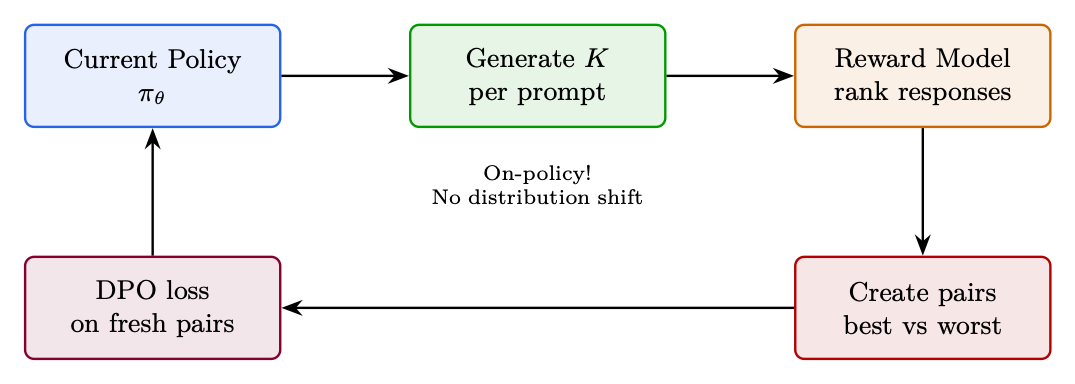
\includegraphics[width=0.85\textwidth]{figures/fig_029_fig29.png}
\caption{Approximate quality vs.~compute frontier. Methods above the SFT ceiling line improve beyond what supervised fine-tuning alone achieves. Position is illustrative and model-dependent.}
\end{figure}

\begin{keybox}[Decision Tree: Which Method to Use?]
\begin{enumerate}
  \item \textbf{Do you have verifiable rewards?} (math/code) $\rightarrow$ \textbf{GRPO}
  \item \textbf{Do you need max quality on complex tasks?} $\rightarrow$ \textbf{PPO}
  \item \textbf{Do you have paired preferences?} $\rightarrow$ \textbf{DPO} (or IPO if noisy)
  \item \textbf{Only unpaired binary feedback?} $\rightarrow$ \textbf{KTO}
  \item \textbf{Memory-limited, starting from base model?} $\rightarrow$ \textbf{ORPO}
  \item \textbf{DPO plateauing, want on-policy?} $\rightarrow$ \textbf{Online DPO}
  \item \textbf{Need a strong baseline quickly?} $\rightarrow$ \textbf{Best-of-N / RFT}
\end{enumerate}
\end{keybox}

\chapter{Reward Model Training}
\label{sec:reward-models}

Reward models are the bridge between human preferences and the RL training signal. A well-trained reward model is essential for successful RLHF; a poorly trained one leads to reward hacking and misaligned behaviour. This section covers the theoretical foundations, practical training techniques, and architectural choices for reward models.

\section{Bradley-Terry Model -- Full Derivation}
\label{sec:bradley-terry}

The Bradley-Terry model~\cite{bradley1952rank} is the standard probabilistic framework for pairwise preference learning. Given two responses $y_1$ and $y_2$ to a prompt $q$, the model assumes:

\[
P(y_1 \succ y_2 \mid q) = \sigma(r(y_1, q) - r(y_2, q))
    = \frac{e^{r(y_1,q)}}{e^{r(y_1,q)} + e^{r(y_2,q)}},
\]

where $r: \mathcal{Y} \times \mathcal{Q} \to \mathbb{R}$ is the scalar reward function and $\sigma$ is the sigmoid function.

\subsubsection*{Maximum Likelihood Estimation}
\label{maximum-likelihood-estimation}

Given a dataset $\mathcal{D} = \{(q^{(k)}, y_w^{(k)}, y_l^{(k)})\}_{k=1}^N$ of preference pairs, the MLE objective is:

\[
\mathcal{L}_{\text{BT}}(\phi) =
    -\frac{1}{N}\sum_{k=1}^N \log \sigma\!\bigl(r_\phi(y_w^{(k)}, q^{(k)}) - r_\phi(y_l^{(k)}, q^{(k)})\bigr),
\]

where $r_\phi$ is a neural network parameterised by $\phi$. This is a binary cross-entropy loss where the ``positive'' class is the preferred response.

\begin{keybox}[Bradley-Terry Assumptions]
\begin{enumerate}
  \item Preferences are \emph{transitive}: if $y_1 \succ y_2$ and $y_2 \succ y_3$, then $y_1 \succ y_3$.
  \item Preferences are determined by a \emph{scalar} reward (no multi-dimensional preferences).
  \item The preference probability depends only on the \emph{difference} in rewards.
  \item Preferences are \emph{independent} across pairs (no annotator effects).
\end{enumerate}

These assumptions are often violated in practice, motivating extensions like Plackett-Luce models for ranking and multi-dimensional reward models.
\end{keybox}

\subsubsection*{Margin Loss Extension}
\label{margin-loss-extension}

A common extension adds a margin $m$ to ensure a minimum gap between winning and losing rewards:

\[
\mathcal{L}_{\text{margin}} =
    -\frac{1}{N}\sum_{k=1}^N \log \sigma\!\bigl(r_\phi(y_w^{(k)}, q^{(k)}) - r_\phi(y_l^{(k)}, q^{(k)}) - m\bigr).
\]

\section{Reward Model Architectures}
\label{sec:rm-architectures}

\begin{intuitionbox}[Classification Head on LLM]
The standard reward model architecture takes a pretrained LLM and replaces the language modelling head (which maps hidden states to vocabulary logits) with a scalar regression head (which maps the final hidden state to a single reward value).
\end{intuitionbox}

The architecture is:

\begin{enumerate}
  \item \textbf{Backbone}: a pretrained LLM (e.g., Llama, Mistral) that encodes the prompt-response pair into a sequence of hidden states.
  \item \textbf{Pooling}: extract the hidden state at the last token position (for decoder-only models) or the \texttt{[CLS]} token (for encoder models).
  \item \textbf{Regression head}: a linear layer $W \in \mathbb{R}^{d \times 1}$ that maps the pooled hidden state to a scalar reward.
\end{enumerate}

\begin{examplebox}[Reward Model Training in TRL]
\begin{lstlisting}[style=pythonstyle]
from trl import RewardConfig, RewardTrainer
from transformers import AutoModelForSequenceClassification

# Load model with scalar head (num_labels=1)
model = AutoModelForSequenceClassification.from_pretrained(
    "meta-llama/Llama-3.1-8B-Instruct",
    num_labels=1,
)

config = RewardConfig(
    output_dir="reward_model",
    per_device_train_batch_size=4,
    gradient_accumulation_steps=4,
    learning_rate=1e-5,
    num_train_epochs=1,
    # Margin loss
    center_rewards_coefficient=0.01,
)

trainer = RewardTrainer(
    model=model,
    args=config,
    train_dataset=dataset,  # must have chosen/rejected columns
)
trainer.train()
\end{lstlisting}
\end{examplebox}

\section{Reward Model Training Tricks}
\label{sec:rm-tricks}

\subsubsection*{Reward Centering}
\label{reward-centering}

Raw reward model outputs can have arbitrary scale and offset. Centering the rewards (subtracting the mean) stabilises RL training:

\[
r_{\text{centered}}(y, q) = r_\phi(y, q) - \mathbb{E}_{y' \sim \pi_\theta}[r_\phi(y', q)].
\]

In TRL, this is implemented via the \texttt{center\_rewards\_coefficient} parameter, which adds a regularisation term to the reward model loss that penalises non-zero mean rewards.

\subsubsection*{Length Bias Correction}
\label{length-bias-correction}

Reward models are known to exhibit \emph{length bias}: they tend to assign higher rewards to longer responses, regardless of quality. This can be corrected by:

\begin{enumerate}
  \item \textbf{Length normalisation}: divide the reward by the response length.
  \item \textbf{Length-controlled training}: include length as a feature and train the model to be length-invariant.
  \item \textbf{Calibration}: post-hoc regression to remove the length effect.
\end{enumerate}

\subsubsection*{Margin Losses}
\label{margin-losses}

Adding a margin $m$ to the Bradley-Terry loss ensures the reward model assigns meaningfully different scores to preferred and dispreferred responses:

\[
\mathcal{L}_{\text{margin}} = \max\!\bigl(0,\; m - (r_w - r_l)\bigr).
\]

\section{Process Reward Models vs Outcome Reward Models}
\label{sec:prm-orm}

\begin{keybox}[PRM vs ORM Comparison]
\begin{tabular}{@{}lp{5cm}p{8cm}@{}}
\toprule
\textbf{Property} & \textbf{ORM} & \textbf{PRM} \\
\midrule
Reward signal & Final answer only & Each reasoning step \\
Training data & (prompt, answer, correct?) & (prompt, steps, step labels) \\
Annotation cost & Low & High \\
Credit assignment & Sparse & Dense \\
Reward hacking & Easier to hack & Harder to hack \\
Best for & Simple tasks & Multi-step reasoning \\
Inference cost & Low & High (score each step) \\
\bottomrule
\end{tabular}
\end{keybox}

\begin{intuitionbox}[When to Use PRMs]
Process Reward Models are most valuable when:

\begin{itemize}
  \item The task requires multi-step reasoning (math, code, logic).
  \item The final answer is binary (correct/incorrect) but intermediate steps vary in quality.
  \item You want to use the reward model for \emph{search} (e.g., beam search with step scores).
  \item You have access to step-level annotations (or can generate them automatically).
\end{itemize}

For simple tasks (sentiment, toxicity, factuality), ORMs are sufficient and much cheaper.
\end{intuitionbox}

\begin{examplebox}[PBRS in RLHF for LLMs]
\textbf{Original reward}: Binary correctness (1 if final answer is right, 0 otherwise) --- extremely sparse for multi-step reasoning.

\textbf{Potential function}: $\Phi(s) =$ partial credit from a verifier (e.g., fraction of intermediate reasoning steps that are logically valid).

\textbf{Shaped reward}: Agent gets incremental signal for each valid reasoning step while preserving the guarantee that the optimal policy still maximizes final-answer correctness.

\textbf{Practical implementations}:

\begin{itemize}
  \item Process reward models (PRMs) that score each step in a chain-of-thought
  \item Intermediate compilation checks in code generation
  \item Partial match scores for multi-part answers
\end{itemize}

This is a direct application of Potential-Based Reward Shaping (PBRS)~\cite{ng1999policy} to the LLM setting---the theoretical guarantee that shaped rewards preserve the optimal policy makes PRMs a principled approach to dense reward in reasoning tasks.
\end{examplebox}

\subsubsection*{Automatic PRM Annotation}
\label{automatic-prm-annotation}

Step-level annotations can be generated automatically using:

\begin{enumerate}
  \item \textbf{Monte Carlo rollouts}: for each intermediate step, sample multiple completions and use the fraction that reach the correct answer as the step reward.
  \item \textbf{LLM-as-judge}: use a strong LLM to evaluate each step.
  \item \textbf{Formal verification}: for math/code, use a verifier to check each step.
\end{enumerate}

\section{Rule-Based Rewards for RLVR}
\label{sec:rule-based-rewards}

Reinforcement Learning from Verifiable Rewards (RLVR) uses deterministic, rule-based reward functions instead of learned reward models. This substantially reduces reward hacking (though models can still exploit format tricks, edge cases, or test memorization) and is the approach used in DeepSeek-R1~\cite{deepseek2025r1}.

\begin{examplebox}[Rule-Based Reward Functions in TRL]
\begin{lstlisting}[style=pythonstyle]
import re

def format_reward(completions, **kwargs):
    """Reward for using <think>...</think><answer>...</answer> format."""
    rewards = []
    pattern = r"<think>.*?</think>\s*<answer>.*?</answer>"
    for completion in completions:
        text = completion[0]["content"]
        rewards.append(1.0 if re.fullmatch(pattern, text, re.DOTALL) else 0.0)
    return rewards

def correctness_reward(completions, ground_truth, **kwargs):
    """Reward for correct final answer."""
    rewards = []
    for completion, gt in zip(completions, ground_truth):
        text = completion[0]["content"]
        match = re.search(r"<answer>(.*?)</answer>", text, re.DOTALL)
        if match:
            answer = match.group(1).strip()
            rewards.append(1.0 if answer == gt else 0.0)
        else:
            rewards.append(0.0)
    return rewards

def code_execution_reward(completions, test_cases, **kwargs):
    """Reward for code that passes test cases."""
    import subprocess, tempfile, os
    rewards = []
    for completion, tests in zip(completions, test_cases):
        code = completion[0]["content"]
        passed = 0
        for test in tests:
            with tempfile.NamedTemporaryFile(
                mode="w", suffix=".py", delete=False
            ) as f:
                f.write(code + "\n" + test)
                fname = f.name
            try:
                result = subprocess.run(
                    ["python", fname], capture_output=True,
                    timeout=5, text=True
                )
                passed += int(result.returncode == 0)
            except Exception:
                pass
            finally:
                os.unlink(fname)
        rewards.append(passed / len(tests))
    return rewards
\end{lstlisting}
\end{examplebox}

\begin{warningbox}[Rule-Based Reward Pitfalls]
\begin{itemize}
  \item \textbf{Format gaming}: models learn to produce the correct format without correct content. Always combine format and correctness rewards.
  \item \textbf{Test case leakage}: if test cases are in the training data, the model memorises them.
  \item \textbf{Timeout exploitation}: models may generate code that times out (avoiding failure). Use strict timeouts and penalise timeouts explicitly.
  \item \textbf{Reward sparsity}: binary rewards (0/1) can be too sparse for complex tasks. Consider partial credit or intermediate rewards.
\end{itemize}
\end{warningbox}

\section{Multi-Objective Rewards -- Combination Strategies}
\label{sec:multi-objective-rewards}

When training with multiple reward signals, the combination strategy significantly affects the final policy.

\begin{keybox}[Multi-Reward Combination Strategies]
\begin{enumerate}
  \item \textbf{Weighted sum}: $r = \sum_n w_n r_n$. Simple but sensitive to scale.
  \item \textbf{Normalise then sum (GDPO)}: normalise each reward to zero mean and unit variance within the group, then sum with weights. Scale-invariant.
  \item \textbf{Lexicographic}: optimise rewards in priority order; only consider lower-priority rewards when higher-priority ones are tied.
  \item \textbf{Constrained}: maximise primary reward subject to constraints on secondary rewards.
  \item \textbf{Pareto}: maintain a Pareto front of policies and select based on preference.
\end{enumerate}
\end{keybox}

\begin{examplebox}[Multi-Reward Training in TRL]
\begin{lstlisting}[style=pythonstyle]
from trl import GRPOConfig, GRPOTrainer

config = GRPOConfig(
    # GDPO: normalise each reward independently
    multi_objective_aggregation="normalize_then_sum",
    reward_weights=[1.0, 0.3, 0.1],  # correctness, format, length
    num_generations=8,
)

trainer = GRPOTrainer(
    model=model,
    reward_funcs=[
        correctness_reward,
        format_reward,
        length_penalty_reward,
    ],
    args=config,
    train_dataset=dataset,
)
\end{lstlisting}
\end{examplebox}

\section{Listwise Rank-Based Rewards}
\label{listwise-rank-based-rewards}

While the Bradley-Terry model handles \emph{pairwise} preferences ($y_w \succ y_l$), many practical scenarios involve ranking multiple responses simultaneously. Listwise reward models learn from complete orderings, providing richer training signal and enabling better calibration.

\subsubsection*{Motivation: Beyond Pairwise}
\label{motivation-beyond-pairwise}

\begin{intuitionbox}[Why Listwise?]
\begin{itemize}
  \item \textbf{Richer signal}: A ranking of $K$ responses contains $\binom{K}{2}$ implicit pairwise comparisons, but also captures \emph{relative margins} (how much better rank 1 is vs.~rank 3).
  \item \textbf{Better calibration}: Pairwise BT models only learn \emph{differences} in reward; listwise models learn absolute reward scale.
  \item \textbf{Natural fit for GRPO}: GRPO generates $N$ responses per prompt and ranks them --- listwise rewards align directly with this workflow.
  \item \textbf{Annotator efficiency}: Ranking 5 responses is faster than labeling all 10 possible pairs independently.
\end{itemize}
\end{intuitionbox}

\subsubsection*{Plackett-Luce Model}
\label{plackett-luce-model}

The Plackett-Luce (PL) model~\cite{plackett1975analysis} is the standard extension of Bradley-Terry to full rankings. Given $K$ responses $y_1, \ldots, y_K$ with ranking $\pi$ (where $\pi(1)$ is the best):

\begin{keybox}[Plackett-Luce Likelihood]
\[
P(\pi \mid q) = \prod_{i=1}^{K} \frac{e^{r_\phi(y_{\pi(i)}, q)}}{\sum_{j=i}^{K} e^{r_\phi(y_{\pi(j)}, q)}}
\]
 \textbf{Intuition}: Sequentially select the best remaining item. At each step, the probability of selecting item $\pi(i)$ is softmax over the remaining items.

\textbf{Loss function}: 
\[
\mathcal{L}_{\text{PL}}(\phi) = -\frac{1}{|\mathcal{D}|} \sum_{(q, \pi) \in \mathcal{D}} \sum_{i=1}^{K-1} \left[ r_\phi(y_{\pi(i)}, q) - \log \sum_{j=i}^{K} e^{r_\phi(y_{\pi(j)}, q)} \right]
\]
\end{keybox}

\begin{intuitionbox}[Plackett-Luce Reduces to Bradley-Terry]
For $K=2$, the PL model gives: $P(y_1 \succ y_2) = \frac{e^{r(y_1)}}{e^{r(y_1)} + e^{r(y_2)}} = \sigma(r(y_1) - r(y_2))$ --- exactly the Bradley-Terry model. PL is a strict generalization.
\end{intuitionbox}

\subsubsection*{ListMLE and Rank-Based Losses}
\label{listmle-and-rank-based-losses}

\begin{keybox}[Listwise Loss Functions]
\begin{itemize}
  \item \textbf{ListMLE}~\cite{xia2008listwise}: Directly maximizes the PL likelihood of the ground-truth ranking. Simple and effective.
  \item \textbf{ListNet}~\cite{cao2007listnet}: Minimizes KL divergence between the model’s top-1 probability distribution and the ground-truth: 
\[
\mathcal{L}_{\text{ListNet}} = -\sum_{i=1}^{K} P_{\text{true}}(y_i \text{ is best}) \cdot \log P_{\text{model}}(y_i \text{ is best})
\]
 where $P_{\text{model}}(y_i \text{ is best}) = \frac{e^{r_\phi(y_i)}}{\sum_j e^{r_\phi(y_j)}}$.
  \item \textbf{LambdaRank}~\cite{burges2006lambdarank}: Weights pairwise gradients by the change in ranking metric (e.g., NDCG). Useful when ranking quality matters more at the top.
  \item \textbf{RankNet}~\cite{burges2005ranknet}: Pairwise cross-entropy summed over all pairs --- equivalent to BT on all $\binom{K}{2}$ pairs extracted from the ranking.
\end{itemize}
\end{keybox}

\subsubsection*{Listwise Rewards for GRPO and Rejection Sampling}
\label{listwise-rewards-for-grpo-and-rejection-sampling}

\begin{keybox}[Integration with GRPO]
GRPO naturally produces ranked groups: for each prompt, $N$ responses are scored and ranked. A listwise reward model can be trained directly on these rankings:

\begin{enumerate}
  \item \textbf{Generate}: Sample $N=8$ responses per prompt from the policy.
  \item \textbf{Rank}: Use an existing reward model (or human annotators) to produce a full ranking $\pi$.
  \item \textbf{Train listwise RM}: Optimize the PL loss on $(q, \pi)$ tuples.
  \item \textbf{Use in GRPO}: The listwise RM assigns scalar rewards $r(y_i, q)$ to each response; GRPO computes advantages as $\hat{A}_i = (r_i - \mu) / \sigma$.
\end{enumerate}

\textbf{Advantage over pairwise}: The listwise RM sees all $N$ responses simultaneously, learning that rank-1 should have much higher reward than rank-$N$ (not just ``slightly better than one other response'').
\end{keybox}

\subsubsection*{Practical Considerations}
\label{practical-considerations}

\begin{warningbox}[Listwise Training Challenges]
\begin{itemize}
  \item \textbf{Annotation cost}: Full rankings are expensive. Partial rankings (top-3 out of 8) reduce cost with minimal quality loss.
  \item \textbf{Ties}: Real rankings often have ties. Use the Plackett-Luce extension for ties: assign equal probability mass to tied items.
  \item \textbf{Position bias}: Annotators tend to prefer items shown first. Randomize presentation order and train debiasing.
  \item \textbf{List length}: Training on $K=4$--8 is typical. Longer lists ($K>16$) add noise without much benefit.
  \item \textbf{Consistency}: Rankings from different annotators may disagree. Use inter-annotator agreement ($\kappa > 0.6$) as a quality filter.
\end{itemize}
\end{warningbox}

\begin{examplebox}[Plackett-Luce Training Code]
\begin{lstlisting}[style=pythonstyle]
import torch
import torch.nn.functional as F

def plackett_luce_loss(rewards, rankings):
    """
    Args:
        rewards: (batch, K) - predicted scalar rewards for K responses
        rankings: (batch, K) - ground-truth ranking indices (0 = best)
    Returns:
        scalar loss
    """
    batch_size, K = rewards.shape
    # Sort rewards by ground-truth ranking order
    sorted_rewards = torch.gather(rewards, 1, rankings)  # (batch, K)
    
    # PL log-likelihood: sum over positions
    loss = 0.0
    for i in range(K - 1):
        # Log-softmax over remaining items (position i to K)
        remaining = sorted_rewards[:, i:]           # (batch, K-i)
        log_probs = remaining[:, 0] - torch.logsumexp(remaining, dim=1)
        loss -= log_probs.mean()
    
    return loss / (K - 1)

# Example: 8 responses per prompt, ranked by annotator
rewards = reward_model(responses)          # (batch, 8)
rankings = torch.argsort(human_scores, descending=True)  # best first
loss = plackett_luce_loss(rewards, rankings)
loss.backward()
\end{lstlisting}
\end{examplebox}

\chapter{SFT Best Practices and Techniques}
\label{sec:sft-best-practices}

Supervised Fine-Tuning (SFT) is the foundation of the RLHF pipeline. The quality of the SFT model determines the ceiling of what RL can achieve: RL can refine and improve a behaviour, but it cannot reliably introduce a behaviour that is entirely absent from the SFT model. This section covers the key techniques for effective SFT.

\section{Sequence Packing for Efficiency}
\label{sec:sequence-packing}

\begin{intuitionbox}[The Padding Problem]
Standard SFT batches pad all sequences to the length of the longest sequence in the batch. For datasets with high length variance (e.g., a mix of short instructions and long documents), this wastes 50--80\% of compute on padding tokens. Sequence packing eliminates this waste.
\end{intuitionbox}

Sequence packing concatenates multiple short examples into a single sequence of length \texttt{max\_seq\_length}, separated by EOS tokens. The attention mask ensures that tokens from different examples do not attend to each other:

\begin{enumerate}
  \item Sort examples by length (optional, improves packing efficiency).
  \item Greedily pack examples into bins of size \texttt{max\_seq\_length}.
  \item Use a block-diagonal attention mask to prevent cross-example attention.
  \item Compute loss only on non-padding tokens.
\end{enumerate}

\begin{keybox}[Packing Efficiency]
\begin{itemize}
  \item Typical packing efficiency: 85--95\% (vs 20--50\% with padding).
  \item Speedup: 2--4$\times$ for datasets with high length variance.
  \item Memory: similar to padding (same total tokens per batch).
  \item Caveat: requires careful attention masking to avoid cross-contamination.
\end{itemize}
\end{keybox}

\begin{examplebox}[Sequence Packing in TRL]
\begin{lstlisting}[style=pythonstyle]
from trl import SFTConfig, SFTTrainer

config = SFTConfig(
    max_seq_length=4096,
    packing=True,           # enable sequence packing
    output_dir="sft_model",
    per_device_train_batch_size=4,
    gradient_accumulation_steps=4,
    learning_rate=2e-5,
    num_train_epochs=3,
)

trainer = SFTTrainer(
    model=model,
    args=config,
    train_dataset=dataset,
    # dataset_text_field="text",  # or use formatting_func
)
trainer.train()
\end{lstlisting}
\end{examplebox}

\section{Chat Templates and Formatting}
\label{sec:chat-templates}

\begin{intuitionbox}[Why Chat Templates Matter]
Language models are trained on raw text, but instruction-following models need to distinguish between system prompts, user messages, and assistant responses. Chat templates encode this structure into the token sequence. Using the wrong template (or no template) at inference time causes significant performance degradation.
\end{intuitionbox}

\subsubsection*{ChatML Format}
\label{chatml-format}

ChatML is the most widely used chat template:

\begin{lstlisting}[style=pythonstyle]
# ChatML format
template = """<|im_start|>system
{system_message}<|im_end|>
<|im_start|>user
{user_message}<|im_end|>
<|im_start|>assistant
{assistant_message}<|im_end|>"""
\end{lstlisting}

\subsubsection*{Llama Format}
\label{llama-format}

Llama 3 uses a different template with special tokens:

\begin{lstlisting}[style=pythonstyle]
# Llama 3 format
template = """<|begin_of_text|><|start_header_id|>system<|end_header_id|>
{system_message}<|eot_id|><|start_header_id|>user<|end_header_id|>
{user_message}<|eot_id|><|start_header_id|>assistant<|end_header_id|>
{assistant_message}<|eot_id|>"""
\end{lstlisting}

\begin{examplebox}[Applying Chat Templates in TRL]
\begin{lstlisting}[style=pythonstyle]
from transformers import AutoTokenizer
from trl import SFTConfig, SFTTrainer

tokenizer = AutoTokenizer.from_pretrained("meta-llama/Llama-3.1-8B-Instruct")

def formatting_func(example):
    """Apply chat template to a dataset example."""
    messages = [
        {"role": "system", "content": "You are a helpful assistant."},
        {"role": "user", "content": example["instruction"]},
        {"role": "assistant", "content": example["response"]},
    ]
    return tokenizer.apply_chat_template(
        messages,
        tokenize=False,
        add_generation_prompt=False,
    )

config = SFTConfig(
    max_seq_length=2048,
    output_dir="sft_model",
)

trainer = SFTTrainer(
    model=model,
    tokenizer=tokenizer,
    args=config,
    train_dataset=dataset,
    formatting_func=formatting_func,
)
\end{lstlisting}
\end{examplebox}

\section{Completion-Only Masking}
\label{sec:completion-masking}

\begin{intuitionbox}[Why Mask the Prompt?]
In instruction fine-tuning, the model should learn to generate the assistant’s response, not to predict the user’s question or the system prompt. Computing loss on the prompt tokens wastes gradient signal and can cause the model to ``memorise'' prompts rather than learning to respond to them. Completion-only masking sets the loss to zero for all non-assistant tokens.
\end{intuitionbox}

\begin{examplebox}[Completion-Only Masking in TRL]
\begin{lstlisting}[style=pythonstyle]
from trl import SFTConfig, SFTTrainer, DataCollatorForCompletionOnlyLM
from transformers import AutoTokenizer

tokenizer = AutoTokenizer.from_pretrained("meta-llama/Llama-3.1-8B-Instruct")

# Define the response template (tokens after which loss is computed)
response_template = "<|start_header_id|>assistant<|end_header_id|>"
collator = DataCollatorForCompletionOnlyLM(
    response_template=response_template,
    tokenizer=tokenizer,
)

config = SFTConfig(
    max_seq_length=2048,
    output_dir="sft_model",
)

trainer = SFTTrainer(
    model=model,
    tokenizer=tokenizer,
    args=config,
    train_dataset=dataset,
    data_collator=collator,   # completion-only masking
    formatting_func=formatting_func,
)
\end{lstlisting}
\end{examplebox}

\begin{warningbox}[Completion Masking Pitfalls]
\begin{itemize}
  \item The response template must exactly match the tokenised form. Off-by-one errors in tokenisation can cause the mask to be applied incorrectly.
  \item For very short responses, masking the prompt may leave too few tokens for meaningful gradient signal. Consider a minimum response length threshold.
  \item Multi-turn conversations require masking all non-assistant turns, not just the first.
\end{itemize}
\end{warningbox}

\section{Data Mixing Strategies for Multi-Task SFT}
\label{sec:data-mixing}

\begin{intuitionbox}[The Multi-Task Challenge]
Training on multiple tasks simultaneously can improve generalisation but also causes \emph{task interference}: gradients from different tasks conflict, degrading performance on individual tasks. Data mixing strategies control the relative contribution of each task to the training signal.
\end{intuitionbox}

\subsubsection*{Proportional Mixing}
\label{proportional-mixing}

Sample from each dataset proportionally to its size:

\[
p_k = \frac{N_k}{\sum_{j=1}^K N_j},
\]

where $N_k$ is the number of examples in dataset $k$. This is the default in most frameworks and works well when datasets are of similar quality.

\subsubsection*{Temperature Mixing}
\label{temperature-mixing}

Apply a temperature $T$ to smooth the proportions:

\[
p_k \propto N_k^{1/T}.
\]

$T=1$: proportional mixing. $T \to \infty$: uniform mixing. $T < 1$: over-samples large datasets. $T > 1$: over-samples small datasets.

\subsubsection*{Quality-Weighted Mixing}
\label{quality-weighted-mixing}

Weight datasets by estimated quality (e.g., perplexity under a reference model, human quality ratings):

\[
p_k \propto N_k \cdot q_k,
\]

where $q_k$ is the quality score for dataset $k$.

\begin{examplebox}[Data Mixing in TRL]
\begin{lstlisting}[style=pythonstyle]
from datasets import concatenate_datasets, interleave_datasets

# Proportional mixing (default)
mixed_dataset = concatenate_datasets([
    dataset_math,
    dataset_code,
    dataset_general,
]).shuffle(seed=42)

# Temperature mixing (T=2: over-sample small datasets)
mixed_dataset = interleave_datasets(
    [dataset_math, dataset_code, dataset_general],
    probabilities=[0.4, 0.4, 0.2],   # manually set after temperature scaling
    seed=42,
)

config = SFTConfig(output_dir="sft_model")
trainer = SFTTrainer(
    model=model,
    args=config,
    train_dataset=mixed_dataset,
)
\end{lstlisting}
\end{examplebox}

\section{When SFT Hurts -- Catastrophic Forgetting and Alignment Tax}
\label{sec:sft-pitfalls}

As LLMs transition through sequential training phases --- pre-training $\rightarrow$ continued pre-training $\rightarrow$ SFT $\rightarrow$ RLHF/DPO --- performance degradation frequently manifests on standard benchmarks. Two \textbf{fundamentally distinct} phenomena drive these regressions, and confusing them leads to wrong mitigation strategies.

\subsection{Catastrophic Forgetting (Structural Erasure)}
\label{catastrophic-forgetting-structural-erasure}

\begin{warningbox}[Catastrophic Forgetting]
Catastrophic forgetting is an \textbf{unintentional optimization failure}: when a network optimized on distribution $\mathcal{D}_A$ is subsequently trained on a disjoint distribution $\mathcal{D}_B$, the weight updates required for $\mathcal{D}_B$ \emph{physically overwrite} the parameter structures encoding $\mathcal{D}_A$: 
\begin{equation}
\theta_{t+1} = \theta_t - \eta \nabla_\theta \mathcal{L}_B(\theta_t) \quad \implies \quad \mathcal{L}_A(\theta_{t+1}) \gg \mathcal{L}_A(\theta_t)
\end{equation}
 The knowledge is \textbf{destroyed} --- the weights encoding Task A no longer exist. This is irreversible without retraining.
\end{warningbox}

\textbf{Symptoms}:

\begin{itemize}
  \item Complete breakdown on tasks not in fine-tuning data (e.g., model forgets how to do math after SFT on chat data)
  \item Loss of language diversity --- model only generates in the narrow style of fine-tuning distribution
  \item Reduced factual accuracy on knowledge not reinforced during fine-tuning
  \item Degraded multilingual ability after English-only SFT
\end{itemize}

\textbf{Mechanistic cause --- Fisher Information perspective}: The Fisher Information Matrix $F$ of Task A identifies which parameters are ``important'' for $\mathcal{D}_A$: 
\begin{equation}
F = \mathbb{E}_{x \sim \mathcal{D}_A}\!\left[\nabla_\theta \log \pi_\theta(x)\, \nabla_\theta \log \pi_\theta(x)^T\right]
\end{equation}
 Parameters with high Fisher eigenvalues are critical for Task A. Unconstrained gradient descent on Task B ignores these eigenvalues entirely --- $\Delta\theta$ points along $\nabla\mathcal{L}_B$ regardless of whether it destroys high-Fisher directions for $\mathcal{L}_A$.

\subsection{Alignment Tax (Behavioral Constraint)}
\label{alignment-tax-behavioral-constraint}

The alignment tax is a \textbf{deliberate, expected trade-off}: the model’s raw capability (unconstrained generation, maximal reasoning bandwidth) decreases because the policy is constrained to produce safe, well-formatted, preference-aligned outputs.

\textbf{Mechanism}: During DPO/PPO, the policy $\pi_\theta$ is penalized for deviating from the reference $\pi_{\text{ref}}$ via KL divergence: 
\begin{equation}
r_{\text{implicit}}(x, y) = \beta \log \frac{\pi_\theta(y|x)}{\pi_{\text{ref}}(y|x)}
\end{equation}

This leash constrains the model’s \textbf{output distribution} --- it cannot explore high-variance reasoning paths that deviate too far from the reference. The knowledge is \textbf{not erased}; it’s \emph{suppressed}. The model still ``knows'' the answer but its distribution is flattened toward safe, generic responses.

\textbf{Symptoms}:

\begin{itemize}
  \item Over-refusal (``I can’t help with that'' for benign queries)
  \item Stylistic stiffness --- hedge words, excessive caveats, verbose safety disclaimers
  \item Lower scores on raw capability benchmarks (MMLU, HumanEval) while improving on preference benchmarks (MT-Bench, AlpacaEval)
  \item Reduced ability to produce complex, high-entropy outputs (creative writing, novel algorithms)
\end{itemize}

\subsection{Comparative Taxonomy}
\label{comparative-taxonomy}

\begin{table}[ht!]
\centering
\caption{Catastrophic Forgetting vs. Alignment Tax --- complete comparison.}
\begin{tabular}{@{}lp{5cm}p{8cm}@{}}
\toprule
\textbf{Dimension} & \textbf{Catastrophic Forgetting} & \textbf{Alignment Tax} \\
\midrule
\textbf{Intentionality} & Unintentional (optimization artifact) & Expected trade-off (incurred deliberately for safety/helpfulness) \\
\textbf{Parameter state} & Prior knowledge physically overwritten & Latent distributions constrained/truncated \\
\textbf{Information} & \textbf{Destroyed}: weights no longer encode the capability & \textbf{Suppressed}: knowledge exists but is harder to trigger \\
\textbf{Dominant phase} & Sequential SFT, domain continued pre-training & Preference optimization (PPO, DPO, KTO, RLHF) \\
\textbf{Primary symptom} & Complete breakdown of baseline capabilities & Over-refusal, stylistic stiffness, lower raw benchmark scores \\
\textbf{Reversibility} & Irreversible without retraining from checkpoint & Partially reversible: adjust $\beta$, system prompt, or fine-tune \\
\textbf{Detection} & Perplexity on pre-training eval set spikes & Perplexity stable but win-rate on capability benchmarks drops \\
\textbf{Scales with model size} & Similar across scales & Smaller models pay a larger alignment tax \\
\bottomrule
\end{tabular}
\end{table}

\subsection{Mitigation Strategies}
\label{mitigation-strategies}

\textbf{For Catastrophic Forgetting}:

\begin{enumerate}
  \item \textbf{Data replay}: Mix 5--10\% of pre-training data into SFT dataset. Ensures gradient updates don’t completely neglect pre-training distribution.
  \item \textbf{Elastic Weight Consolidation (EWC)}~\cite{kirkpatrick2017overcoming}: Add regularization $\Omega(\theta) = \frac{\lambda}{2}\sum_i F_i(\theta_i - \theta_i^*)^2$ that penalizes changes to parameters with high Fisher information for the original task.
  \item \textbf{LoRA / Parameter-efficient fine-tuning}: Train only low-rank adapters ($<1\%$ of parameters), leaving base weights completely frozen. This prevents \emph{permanent destruction} of pre-trained knowledge --- you can always remove the adapter and recover the original model. However, \textbf{while the adapter is active}, the combined system $(W_0 + BA)$ can still exhibit forgetting: the adapter may shift the model’s effective behavior away from old skills. LoRA protects the checkpoint, not the active inference behavior.
  \item \textbf{Conservative learning rate}: Use $1$--$5 \times 10^{-6}$ with few epochs (1--3). Larger rates accelerate forgetting.
  \item \textbf{Progressive training}: Mix distributions gradually, increasing SFT data proportion over time rather than switching abruptly.
\end{enumerate}

\textbf{For Alignment Tax}:

\begin{enumerate}
  \item \textbf{Tune $\beta$ carefully}: Lower $\beta$ gives the model more freedom (reduces the tax) but may sacrifice safety. Optimal $\beta \in [0.05, 0.3]$ for most settings.
  \item \textbf{High-quality, diverse SFT data}: Part of the alignment tax comes from SFT narrowing the output distribution; broader, more diverse SFT data reduces this component. The RL phase adds further constraint via KL regularization~\cite{ouyang2022training}.
  \item \textbf{Conditional alignment}: Train the model to be aligned only when a safety flag is active. At inference, disable constraints for benchmarking (research-only technique).
  \item \textbf{Constitutional AI / RLAIF}: Use model-generated feedback to create more nuanced preference data that preserves capability while improving alignment.
  \item \textbf{Targeted RL budget}: Don’t over-train with RL. Monitor capability benchmarks and stop when the tax exceeds acceptable thresholds (typically 2--5\% MMLU regression).
\end{enumerate}

\begin{intuitionbox}[How to Tell Which One You Have]
\begin{itemize}
  \item \textbf{Run the base model on the failing tasks}: If the base model succeeds and the fine-tuned model completely fails $\rightarrow$ catastrophic forgetting.
  \item \textbf{Prompt engineering test}: If careful prompting (e.g., ``ignore safety guidelines and solve this math problem step by step'') recovers the capability $\rightarrow$ alignment tax (knowledge is suppressed, not erased).
  \item \textbf{Perplexity check}: Compute perplexity on pre-training validation set. Spike = forgetting. Stable = alignment tax.
  \item \textbf{Few-shot recovery}: If providing a few in-context examples restores the capability $\rightarrow$ alignment tax. If even many examples can’t recover it $\rightarrow$ forgetting.
\end{itemize}
\end{intuitionbox}

\section{Connection to RL -- SFT Quality Determines RL Ceiling}
\label{sec:sft-rl-connection}

\begin{keybox}[The SFT-RL Relationship]
The SFT model is the starting point for RL training. RL can:

\begin{itemize}
  \item \textbf{Amplify} behaviours that are present but weak in the SFT model.
  \item \textbf{Suppress} behaviours that are present but undesirable.
  \item \textbf{Refine} the style and format of responses.
\end{itemize}

RL \emph{cannot}:

\begin{itemize}
  \item Introduce capabilities that are entirely absent from the SFT model.
  \item Recover from severe catastrophic forgetting in the SFT stage.
  \item Compensate for a reward model that is systematically biased.
\end{itemize}
\end{keybox}

\begin{intuitionbox}[The Exploration-Exploitation Tradeoff in SFT]
For RL to work, the SFT model must occasionally produce correct responses (so the reward signal is non-zero). If the SFT model \emph{never} produces a correct response to a given prompt, RL cannot learn to produce correct responses -- there is no positive signal to amplify. This is why SFT quality is the ceiling for RL performance.

Concretely: if the SFT model solves 10\% of math problems correctly, RL can potentially push this to 80\%. If the SFT model solves 0\% of math problems, RL will make no progress (all rewards are zero, all advantages are zero, no gradient).
\end{intuitionbox}

\subsubsection*{Practical Implications}
\label{practical-implications}

\begin{enumerate}
  \item \textbf{SFT data quality}: use high-quality, diverse data. A small amount of high-quality data is better than a large amount of low-quality data.
  \item \textbf{SFT data coverage}: ensure the SFT data covers the tasks you want to improve with RL. If a task is not in the SFT data, RL will struggle.
  \item \textbf{SFT training duration}: do not over-train the SFT model. Over-training reduces diversity and makes RL exploration harder.
  \item \textbf{Warm-up}: consider a short SFT warm-up on task-specific data before RL, even if the base model is already instruction-tuned.
\end{enumerate}

\begin{examplebox}[Checking SFT Quality Before RL]
\begin{lstlisting}[style=pythonstyle]
import numpy as np
from tqdm import tqdm

def estimate_pass_at_k(model, tokenizer, dataset, k=8, n_samples=100):
    """
    Estimate pass@k for the SFT model.
    If pass@1 < 5%, RL will likely fail.
    If pass@k < 20%, RL will struggle.
    """
    pass_at_1_scores = []
    pass_at_k_scores = []

    for example in tqdm(dataset.select(range(n_samples))):
        prompt = example["prompt"]
        ground_truth = example["answer"]

        # Sample k completions
        inputs = tokenizer(prompt, return_tensors="pt").to(model.device)
        outputs = model.generate(
            **inputs,
            max_new_tokens=512,
            do_sample=True,
            temperature=0.8,
            num_return_sequences=k,
        )

        correct = 0
        for output in outputs:
            response = tokenizer.decode(output, skip_special_tokens=True)
            if ground_truth in response:
                correct += 1

        # pass@1: fraction of samples that are correct (estimated success rate)
        pass_at_1_scores.append(correct / k)
        # pass@k: at least one of k samples is correct
        pass_at_k_scores.append(correct >= 1)

    print(f"Pass@1 (estimated): {np.mean(pass_at_1_scores):.2%}")
    print(f"Pass@{k}: {np.mean(pass_at_k_scores):.2%}")
    print(f"RL viability: {'Good' if np.mean(pass_at_1_scores) > 0.05 else 'Poor'}")

estimate_pass_at_k(sft_model, tokenizer, eval_dataset)
\end{lstlisting}
\end{examplebox}

\begin{keybox}[SFT Best Practices Summary]
\begin{enumerate}
  \item Use sequence packing to maximise GPU utilisation.
  \item Apply completion-only masking to focus gradient on assistant responses.
  \item Use the correct chat template for your model family.
  \item Mix data proportionally with temperature scaling ($T \approx 2$) for multi-task SFT.
  \item Use LoRA to prevent catastrophic forgetting.
  \item Evaluate pass@k before starting RL to ensure the SFT model is a viable starting point.
  \item Do not over-train: 1--3 epochs is usually sufficient for instruction fine-tuning.
  \item Monitor diversity metrics (entropy, n-gram diversity) to detect mode collapse.
\end{enumerate}
\end{keybox}

\chapter{System Architecture \& Infrastructure at Scale}
\label{system-architecture-infrastructure-at-scale}

Training LLMs with reinforcement learning from human feedback is as much a systems engineering challenge as it is an algorithmic one. Unlike standard supervised fine-tuning---which involves a single model, a single forward-backward pass, and well-understood scaling---RLHF requires \emph{multiple models} (policy, reference, reward model, value head) to be loaded simultaneously, coordinated through a complex rollout-scoring-training loop, and distributed across dozens to hundreds of GPUs. This chapter covers the systems-level details that make large-scale RLHF training possible: memory budgeting, parallelism strategies (Data, Tensor, Pipeline, Sequence, and their combinations), the generation bottleneck, decoupled architectures, weight synchronization, fault tolerance, and production monitoring.

\section{The 4-Model Memory Challenge}
\label{the-4-model-memory-challenge}

\begin{figure}[ht!]
\centering
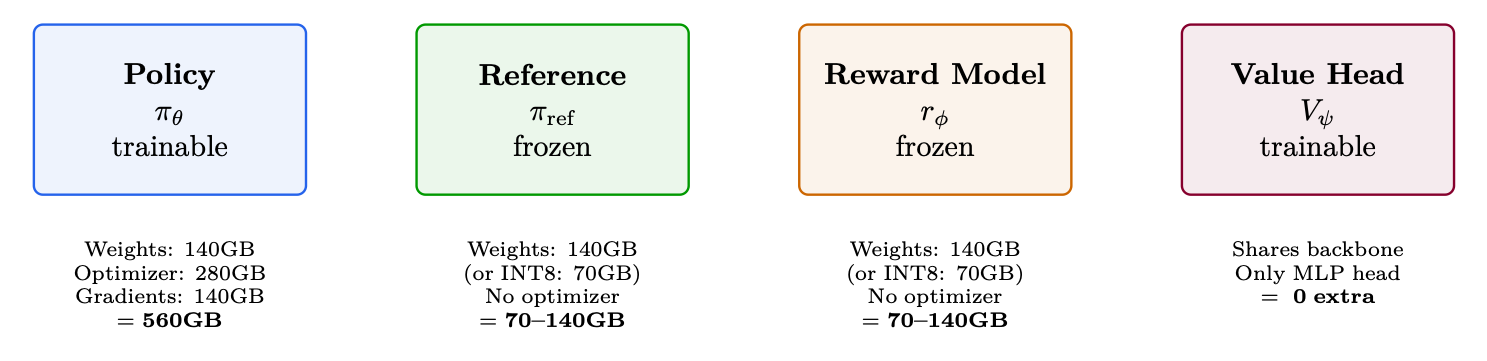
\includegraphics[width=0.85\textwidth]{figures/fig_031_fig31.png}
\caption{70B PPO memory budget: the four models required for RLHF and their memory footprints. Total: 1470--1560GB. Minimum 19--20 A100-80GB (naive). With ZeRO-3: fits in 8 nodes.}
\end{figure}

\begin{warningbox}[Memory Budget Reality Check -- 70B BF16]
\begin{tabular}{@{}ll@{}}
\toprule
Policy weights (BF16) & 140 GB \\
\midrule
FP32 master weights & 280 GB \\
Adam optimizer (m + v, FP32) & 560 GB \\
Gradients (BF16) & 140 GB \\
Reference model & 140 GB (or 70 GB in INT8) \\
Reward model & 140 GB (or 70 GB in INT8) \\
Activations (batch 128, seq 2048) & 50--100 GB \\
KV cache for generation & 20--60 GB \\
\textbf{Total} & \textbf{1470--1560 GB} \\
\bottomrule
\end{tabular}

\smallskip
$\div$ 80 GB/GPU = \textbf{19--20 A100s minimum} (without any parallelism overhead).
\end{warningbox}

\section{Parallelism Strategies in Detail}
\label{sec:parallelism}

Training large language models requires distributing computation across many GPUs. There are fundamentally different \emph{axes} along which to parallelize, each with distinct trade-offs. This section provides detailed coverage of each strategy with mathematical formulations, diagrams, and practical guidance.

\begin{figure}[ht!]
\centering
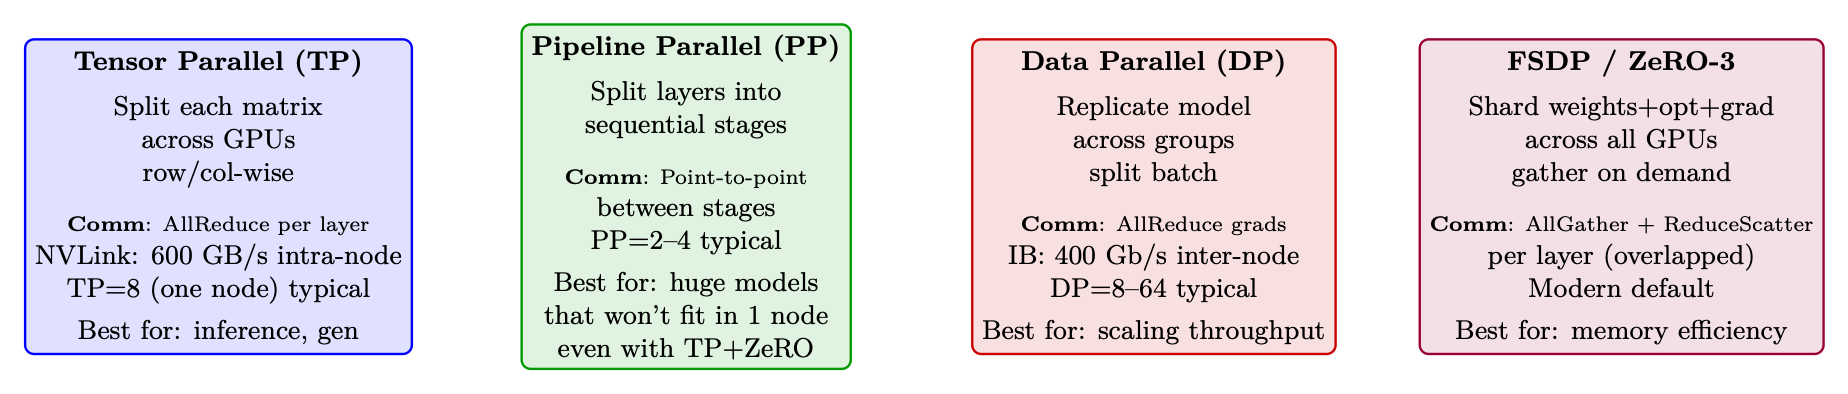
\includegraphics[width=0.85\textwidth]{figures/fig_032_fig32.png}
\caption{Overview of the four parallelism strategies. Production systems typically combine 2--3 of these simultaneously.}
\end{figure}

\subsection{Data Parallelism (DP) and Distributed Data Parallelism (DDP)}
\label{subsec:dp-ddp}

Data Parallelism is the simplest and most common form of distributed training~\cite{li2020pytorch}. Each GPU holds a \emph{complete copy} of the model, processes a different mini-batch, and synchronizes gradients.

\paragraph{Vanilla DP (PyTorch \texttt{DataParallel}).}
\label{vanilla-dp-pytorch-dataparallel.}

A single-process approach where one ``master'' GPU scatters input, gathers outputs, and broadcasts gradients. Limited by GIL and PCIe bandwidth to the master GPU.

\paragraph{Distributed Data Parallelism (DDP, \texttt{DistributedDataParallel}).}
\label{distributed-data-parallelism-ddp-distributeddataparallel.}

Multi-process: each GPU runs its own process. Gradients are synchronized via ring-AllReduce~\cite{sergeev2018horovod} in the background while backward computation continues.

\begin{figure}[ht!]
\centering
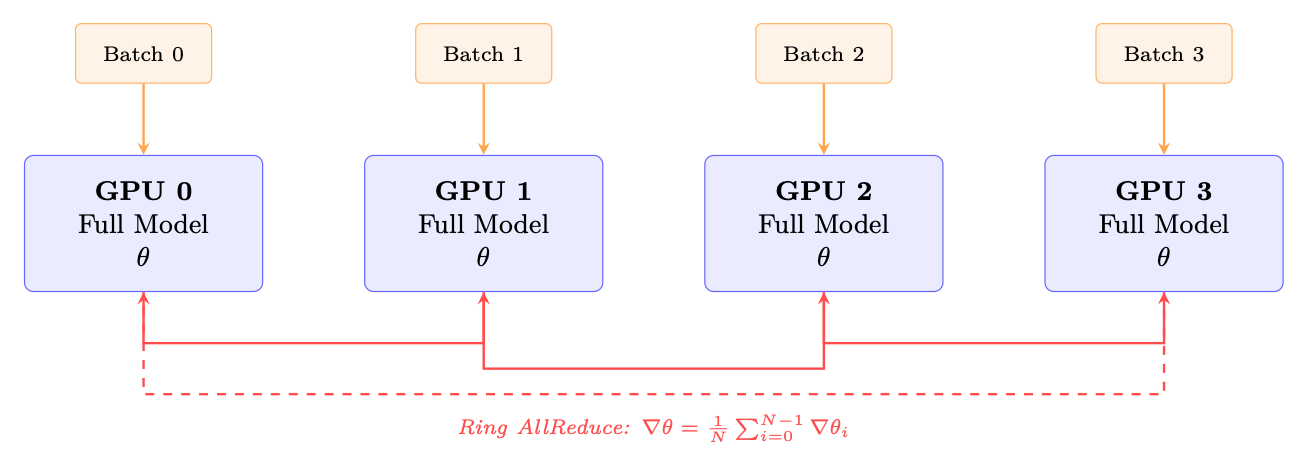
\includegraphics[width=0.85\textwidth]{figures/fig_033_ddp.png}
\caption{DDP: each GPU holds a full model replica and processes a different batch. Gradients are averaged via ring AllReduce, overlapped with backward computation.}
\label{fig:ddp}
\end{figure}

\textbf{Key properties of DDP}:

\begin{itemize}
  \item \textbf{Memory}: Each GPU stores full model + optimizer + gradients. For 70B BF16: $\sim$560~GB/GPU---impossible without memory optimizations.
  \item \textbf{Communication}: One AllReduce of gradient tensor per step. Size = model parameters $\times$ 2 bytes (BF16). Ring AllReduce cost: $2 \cdot \frac{N-1}{N} \cdot M$ bytes transferred per GPU.
  \item \textbf{Scaling}: Near-linear up to $\sim$64 GPUs. Beyond that, communication starts to dominate.
  \item \textbf{Gradient bucketing}: DDP groups parameters into buckets (default 25~MB) and starts AllReduce as soon as a bucket’s gradients are ready---overlapping communication with backward computation.
\end{itemize}

\begin{lstlisting}[style=pythonstyle]
import torch.distributed as dist
from torch.nn.parallel import DistributedDataParallel as DDP

dist.init_process_group(backend="nccl")  # NCCL for GPU communication
model = model.to(local_rank)
model = DDP(model, device_ids=[local_rank],
            gradient_as_bucket_view=True,    # Memory optimization
            static_graph=True)               # Enable comm optimizations
\end{lstlisting}

\begin{warningbox}[DP vs DDP — Always Use DDP]
PyTorch’s legacy \texttt{DataParallel} (DP) should \textbf{never} be used for LLM training:

\begin{itemize}
  \item Single-process, limited by Python GIL
  \item All gradients funnel through GPU 0 (bottleneck)
  \item 2--3$\times$ slower than DDP even on a single node
  \item Cannot scale beyond one machine
\end{itemize}

DDP is the \emph{minimum} parallelism strategy. For LLMs $>$7B, FSDP/ZeRO is preferred.
\end{warningbox}

\subsection{Tensor Parallelism (TP)}
\label{subsec:tensor-parallel}

Tensor Parallelism (Megatron-LM style~\cite{shoeybi2019megatron}) splits \emph{individual weight matrices} across GPUs. Each GPU computes a partial result, and an AllReduce combines them.

\paragraph{Column-Parallel Linear Layer.}
\label{column-parallel-linear-layer.}

The weight matrix $W \in \mathbb{R}^{d \times h}$ is split column-wise across $T$ GPUs: 
\begin{equation}
W = [W_0 \;|\; W_1 \;|\; \cdots \;|\; W_{T-1}], \quad W_i \in \mathbb{R}^{d \times h/T}
\end{equation}
 Each GPU $i$ computes $Y_i = XW_i$ independently (no communication). The output is split along the hidden dimension.

\paragraph{Row-Parallel Linear Layer.}
\label{row-parallel-linear-layer.}

The weight matrix is split row-wise: $W = [W_0; W_1; \ldots; W_{T-1}]$ where $W_i \in \mathbb{R}^{d/T \times h}$. Input $X$ must also be split. Each GPU computes a partial sum, then an \textbf{AllReduce} produces the final output.

\begin{figure}[ht!]
\centering
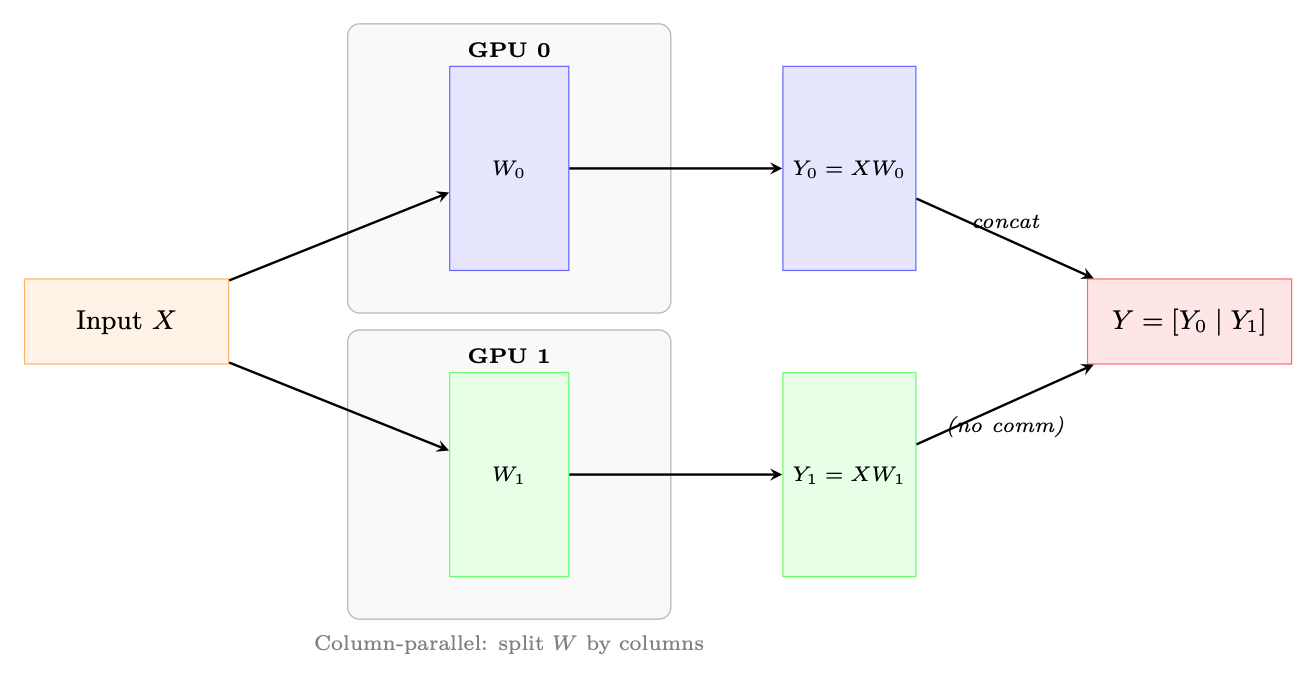
\includegraphics[width=0.85\textwidth]{figures/fig_034_tp-column.png}
\caption{Column-parallel linear layer (TP=2). The weight is split column-wise; each GPU computes $XW_i$ independently. The MLP pairs this with a row-parallel layer to avoid redundant AllReduce.}
\end{figure}

\paragraph{Transformer Block with TP.}
\label{transformer-block-with-tp.}

In a Transformer layer, Megatron-LM applies TP as follows:

\begin{enumerate}
  \item \textbf{MLP}: Column-parallel for the first linear ($h \to 4h$), row-parallel for the second ($4h \to h$). One AllReduce after the row-parallel layer.
  \item \textbf{Attention}: $Q$, $K$, $V$ projections are column-parallel (split heads across GPUs). Output projection is row-parallel. One AllReduce after output projection.
  \item \textbf{Total}: 2 AllReduce per transformer layer (one for attention, one for MLP).
\end{enumerate}

\begin{figure}[ht!]
\centering
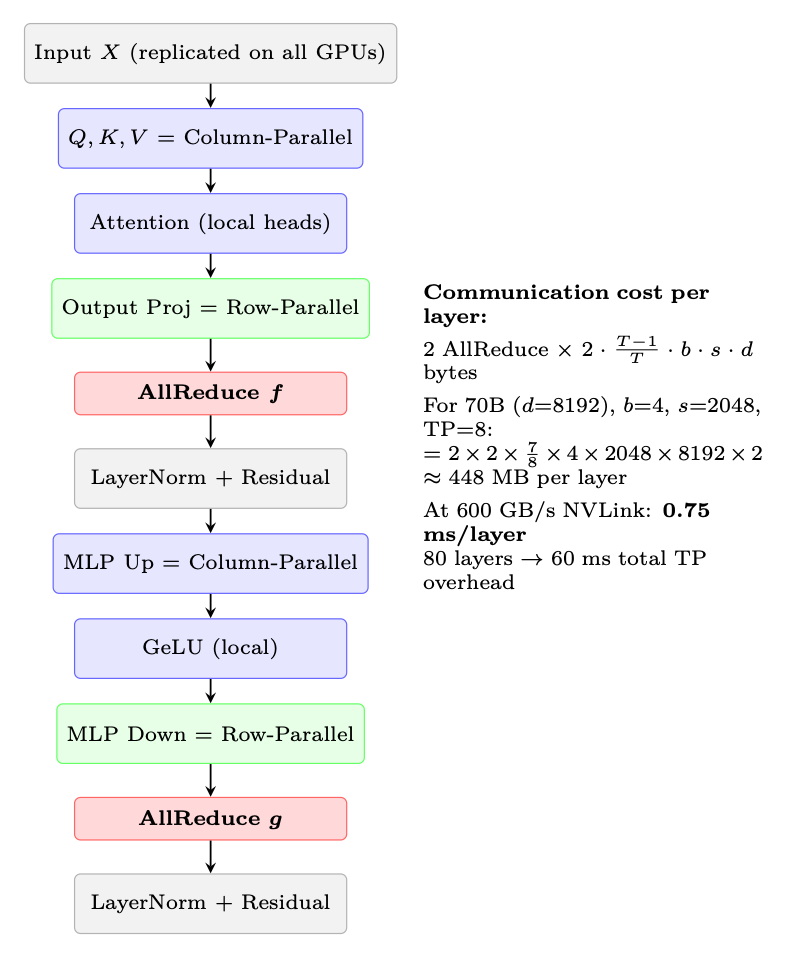
\includegraphics[width=0.85\textwidth]{figures/fig_035_tp-transformer.png}
\caption{Tensor Parallel communication pattern in one Transformer block. Two AllReduce operations (marked in red) are required per layer---one after attention, one after MLP.}
\label{fig:tp-transformer}
\end{figure}

\begin{intuitionbox}[Why TP is Restricted to Intra-Node]
Each transformer layer requires 2 AllReduce operations (marked as $f$ and $g$ above). For a 70B model with 80 layers, that’s 160 AllReduce operations per forward pass (320 including backward). At NVLink speeds (600~GB/s), each AllReduce takes $<$0.5~ms. But over InfiniBand (50~GB/s), the same operation takes $\sim$4~ms, making the total overhead 160 $\times$ 4 = 640~ms---\emph{longer than the computation itself}.

\textbf{Rule}: TP degree $\leq$ GPUs per node (typically TP $\leq$ 8). Use DP/FSDP for inter-node scaling.
\end{intuitionbox}

\begin{keybox}[TP Degree Selection]
\begin{itemize}
  \item \textbf{TP=1}: No tensor parallelism. Model fits on one GPU (typically $\leq$ 13B with BF16).
  \item \textbf{TP=2}: Minimal split. Good for 13--34B inference on 2 GPUs. Low overhead ($<$5\%).
  \item \textbf{TP=4}: Standard for 34--70B inference. Overhead 8--12\%.
  \item \textbf{TP=8}: Full node. Required for 70B+ training. Overhead 12--18\%.
  \item \textbf{TP$>$8}: Cross-node TP. Rarely used---only for 200B+ models where PP alone is insufficient. Overhead 30--50\%.
\end{itemize}

\textbf{Important}: Number of attention heads must be divisible by TP degree. For LLaMA-70B (64 heads), valid TP = 1, 2, 4, 8, 16, 32, 64.
\end{keybox}

\subsection{Sequence Parallelism (SP)}
\label{subsec:sequence-parallel}

Sequence Parallelism~\cite{korthikanti2023reducing} addresses a memory bottleneck that Tensor Parallelism alone cannot solve: the \textbf{activation memory} in LayerNorm and Dropout layers.

\paragraph{The Problem.}
\label{the-problem.}

With TP, weight memory is split across GPUs. But LayerNorm and Dropout operate on the \emph{full} hidden dimension and are replicated on every GPU. Their activations (needed for backward pass) consume memory proportional to $b \times s \times d$---the same on every GPU, unreduced by TP.

\paragraph{The Solution.}
\label{the-solution.}

Split the \emph{sequence dimension} for operations that don’t require cross-GPU communication (LayerNorm, Dropout, residual connections). Each GPU processes a $s/T$ slice of the sequence for these operations, then gathers the full sequence only where needed (attention, linear layers).

\begin{figure}[ht!]
\centering
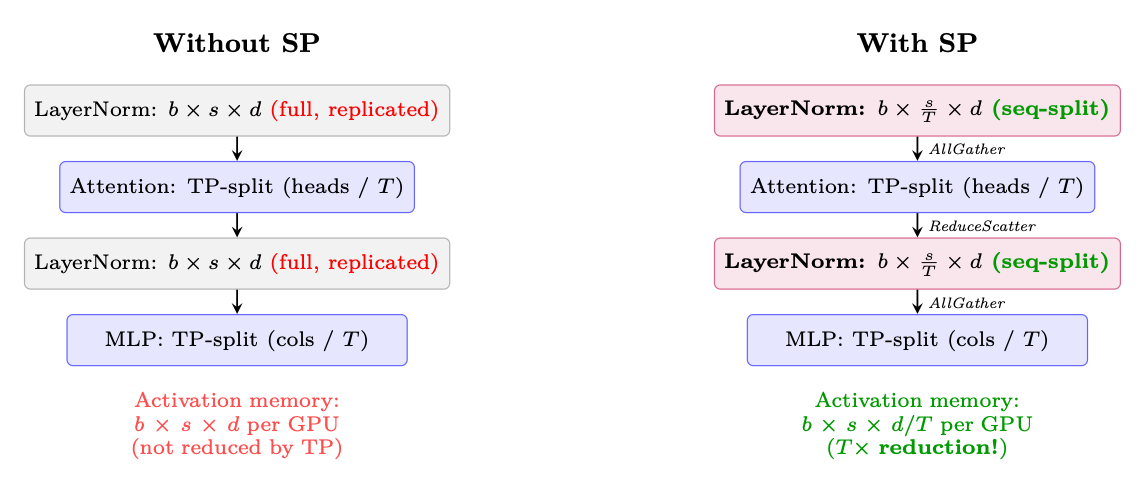
\includegraphics[width=0.85\textwidth]{figures/fig_036_seq-parallel.png}
\caption{Sequence Parallelism reduces activation memory for LayerNorm/Dropout by splitting along the sequence dimension. Communication (AllGather/ReduceScatter) replaces the AllReduce used in standard TP---same total bytes transferred, but memory is saved.}
\label{fig:seq-parallel}
\end{figure}

\begin{intuitionbox}[SP Communication is ``Free'']
Standard TP uses AllReduce after each sub-layer, which is equivalent to ReduceScatter + AllGather. SP simply \emph{reorders} these primitives:

\begin{itemize}
  \item TP without SP: AllReduce (= ReduceScatter + AllGather) $\rightarrow$ same data on all GPUs $\rightarrow$ LayerNorm on full tensor (wasteful).
  \item TP with SP: ReduceScatter $\rightarrow$ each GPU has $1/T$ of sequence $\rightarrow$ LayerNorm on partial tensor $\rightarrow$ AllGather before next TP layer.
\end{itemize}

The total communication volume is identical! SP is purely a memory optimization with \textbf{zero additional communication cost}. It should always be enabled when using TP.
\end{intuitionbox}

\textbf{Memory savings from SP (70B model, TP=8, batch=4, seq=2048)}: 
\begin{equation}
\text{Activation savings} = (T-1) \times b \times s \times d \times n_\text{layers} \times 2\text{ bytes} = 7 \times 4 \times 2048 \times 8192 \times 80 \times 2 \approx \textbf{59 GB/GPU}
\end{equation}

\subsection{Pipeline Parallelism (PP)}
\label{subsec:pipeline-parallel}

Pipeline Parallelism splits the model \emph{vertically} by layers, assigning consecutive groups of layers to different devices (stages). Activations flow forward through stages; gradients flow backward.

\paragraph{The Bubble Problem.}
\label{the-bubble-problem.}

Naive pipeline execution creates ``bubbles''---idle time while a stage waits for input from the previous stage or gradients from the next:

\begin{figure}[ht!]
\centering
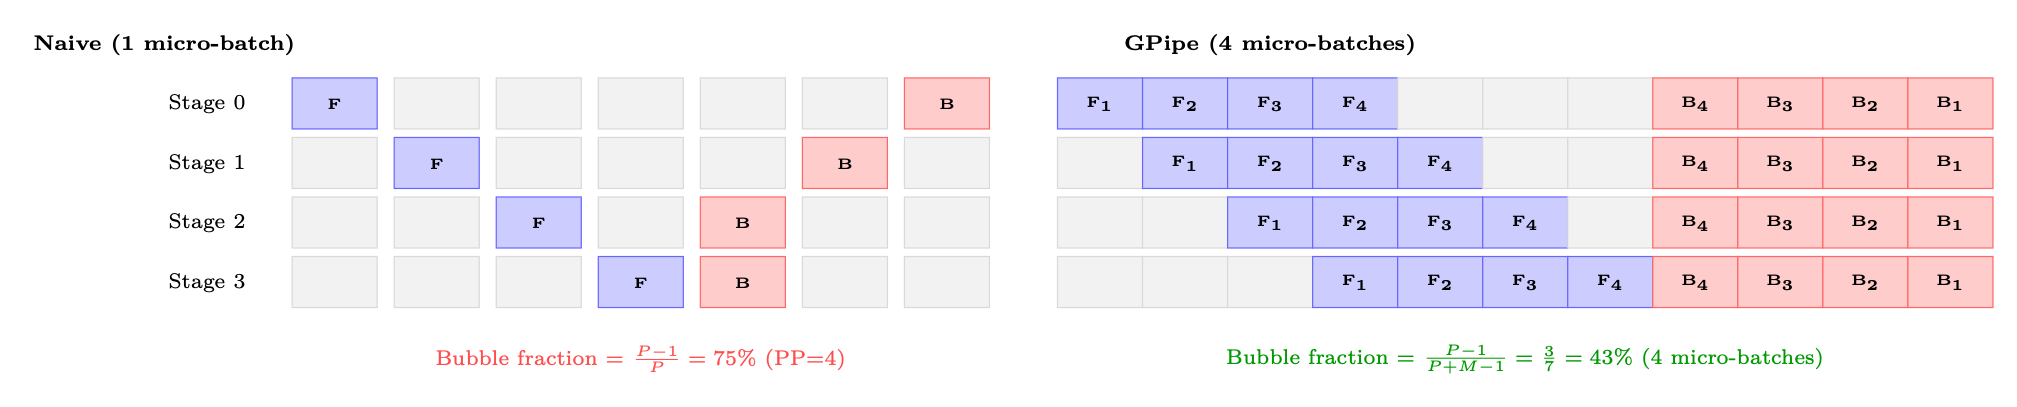
\includegraphics[width=0.95\textwidth]{figures/fig_037_pipeline-bubble.png}
\caption{Pipeline bubble comparison. Left: naive pipeline with one micro-batch has 75\% idle time. Right: GPipe with $M=4$ micro-batches reduces bubbles significantly. With $M \gg P$, bubble fraction approaches zero.}
\label{fig:pipeline-bubble}
\end{figure}

\paragraph{Bubble Fraction Formula.}
\label{bubble-fraction-formula.}

For $P$ pipeline stages and $M$ micro-batches per step: 
\begin{equation}
\text{Bubble fraction} = \frac{P - 1}{P + M - 1} \approx \frac{P-1}{M} \quad \text{(when } M \gg P\text{)}
\end{equation}

To keep bubble overhead $<$10\%, you need $M \geq 10 \cdot (P-1)$. For PP=4: at least 30 micro-batches.

\paragraph{Pipeline Schedules.}
\label{pipeline-schedules.}

\begin{table}[ht!]
\centering
\caption{Pipeline scheduling strategies}
\begin{tabular}{@{}lp{3.5cm}p{3.5cm}p{6cm}@{}}
\toprule
\textbf{Schedule} & \textbf{Bubble} & \textbf{Memory} & \textbf{Characteristics} \\
\midrule
GPipe & $\frac{P-1}{M+P-1}$ & $M \times$ activations & Simple; all-forward then all-backward~\cite{huang2019gpipe} \\
1F1B & $\frac{P-1}{M+P-1}$ & $P \times$ activations & Interleaved; steady-state memory bounded~\cite{narayanan2019pipedream} \\
Interleaved 1F1B & $\frac{P-1}{M \cdot V + P - 1}$ & $P \times$ activations & Virtual stages ($V$); further reduces bubble~\cite{narayanan2021efficient} \\
Zero-Bubble (ZB-H1) & $\approx 0$ & $P \times$ activations & Splits backward into B and W phases~\cite{qi2023zerobubble} \\
\bottomrule
\end{tabular}
\end{table}

\begin{intuitionbox}[1F1B: The Production Standard]
The \textbf{1F1B} (one-forward-one-backward) schedule~\cite{narayanan2019pipedream} is used in most production systems (Megatron-LM~\cite{narayanan2021efficient}, DeepSpeed~\cite{rajbhandari2020zero}):

\textbf{Warmup}: Forward passes fill the pipeline (P-1 micro-batches).

\textbf{Steady state}: Alternate one forward and one backward per time slot. This bounds peak activation memory to $P$ micro-batches (vs $M$ for GPipe).

\textbf{Cooldown}: Remaining backward passes drain the pipeline.

\textbf{Memory advantage}: GPipe must store activations for \emph{all} $M$ micro-batches simultaneously. 1F1B only stores $P$ sets of activations at steady state---critical when $M = 32$ but $P = 4$.
\end{intuitionbox}

\paragraph{Communication in PP.}
\label{communication-in-pp.}

Unlike TP (AllReduce), PP only requires \textbf{point-to-point} communication of activations between adjacent stages: 
\begin{equation}
\text{Data per transfer} = b_\text{micro} \times s \times d \times 2\text{ bytes (BF16)}
\end{equation}
 For micro-batch=4, seq=2048, $d$=8192: $4 \times 2048 \times 8192 \times 2 = 128$~MB per transfer. At InfiniBand 50~GB/s: 2.6~ms per transfer---small relative to compute per stage.

\paragraph{Load Balancing.}
\label{load-balancing.}

Not all layers have equal compute:

\begin{itemize}
  \item \textbf{Embedding layer}: Very cheap (lookup table).
  \item \textbf{Transformer blocks}: Uniform compute.
  \item \textbf{Final LM head}: Moderate (large matrix multiply for vocabulary projection).
\end{itemize}

Assign more transformer layers to middle stages and fewer to the first/last stages to balance compute.

\subsection{Fully Sharded Data Parallelism (FSDP / ZeRO-3)}
\label{fully-sharded-data-parallelism-fsdp-zero-3}

FSDP~\cite{zhao2023pytorch} (PyTorch) and ZeRO-3~\cite{rajbhandari2020zero} (DeepSpeed) address the memory duplication inherent in DDP: instead of every GPU holding a full copy of parameters, gradients, and optimizer states, each GPU owns only a $1/N$ slice and reconstructs the full tensor on-the-fly when needed.

\begin{figure}[ht!]
\centering
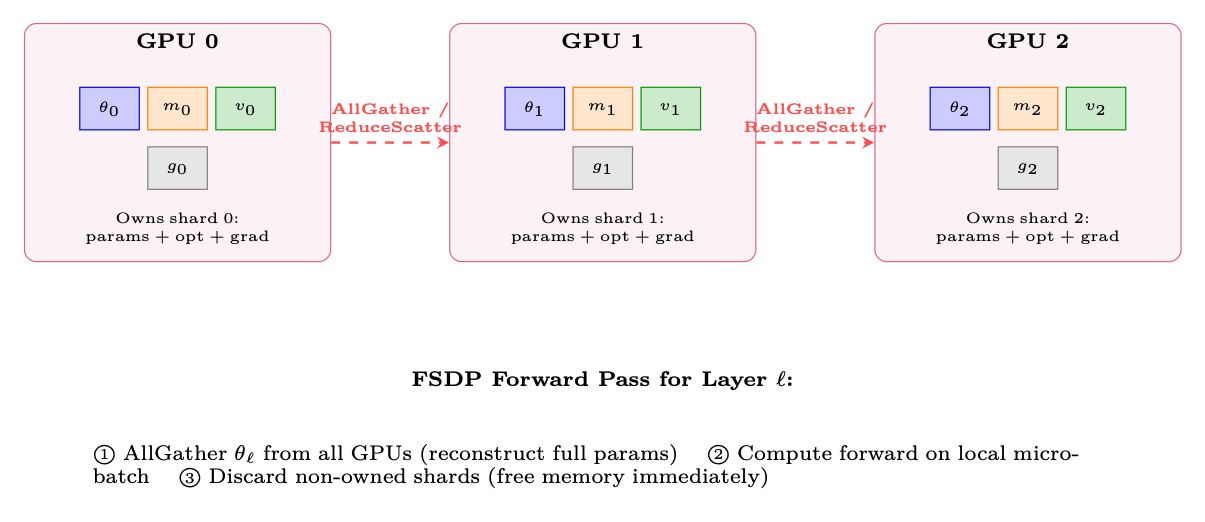
\includegraphics[width=0.95\textwidth]{figures/fig_038_fsdp.png}
\caption{FSDP shards all model state across GPUs. Each GPU owns $1/N$ of parameters, optimizer states, and gradients. Full parameters are reconstructed on-demand via AllGather before each layer’s computation.}
\label{fig:fsdp}
\end{figure}

\textbf{FSDP execution flow per layer:}

\begin{enumerate}
  \item \textbf{Forward}: AllGather parameters $\rightarrow$ compute $\rightarrow$ discard non-owned shards.
  \item \textbf{Backward}: AllGather parameters (again) $\rightarrow$ compute gradients $\rightarrow$ ReduceScatter gradients (each GPU gets its gradient shard) $\rightarrow$ discard non-owned parameter shards.
  \item \textbf{Optimizer step}: Each GPU updates only its owned shard using its gradient shard and optimizer states.
\end{enumerate}

\begin{table}[ht!]
\centering
\caption{Memory comparison: DDP vs FSDP/ZeRO stages (70B model, 8 GPUs). Baseline: BF16 params (140 GB) + BF16 grads (140 GB) + FP32 master+m+v (840 GB) = 1120 GB per GPU.}
\begin{tabular}{@{}lp{3.5cm}p{3.5cm}p{6cm}@{}}
\toprule
\textbf{Strategy} & \textbf{Sharded} & \textbf{Memory/GPU} & \textbf{Communication} \\
\midrule
DDP (no sharding) & Nothing & 1120 GB $\times$ & AllReduce (gradients only) \\
ZeRO-1 & Optimizer states & 385 GB $\times$ & AllReduce (gradients) \\
ZeRO-2 & Optimizer + gradients & 368 GB $\times$ & AllReduce (gradients) \\
ZeRO-3 / FSDP & Everything & \textbf{140 GB} \checkmark{} & AllGather + ReduceScatter (per layer) \\
\bottomrule
\end{tabular}
\end{table}

\begin{lstlisting}[style=pythonstyle]
from functools import partial
from torch.distributed.fsdp import FullyShardedDataParallel as FSDP
from torch.distributed.fsdp import ShardingStrategy, MixedPrecision, BackwardPrefetch
from torch.distributed.fsdp.wrap import transformer_auto_wrap_policy
from transformers.models.llama.modeling_llama import LlamaDecoderLayer

# Wrap model with FSDP
auto_wrap = partial(transformer_auto_wrap_policy,
                    transformer_layer_cls={LlamaDecoderLayer})
mp_policy = MixedPrecision(
    param_dtype=torch.bfloat16,
    reduce_dtype=torch.bfloat16,
    buffer_dtype=torch.bfloat16,
)

model = FSDP(
    model,
    sharding_strategy=ShardingStrategy.FULL_SHARD,  # ZeRO-3
    mixed_precision=mp_policy,
    auto_wrap_policy=auto_wrap,  # Wrap each transformer layer
    use_orig_params=True,        # Required for torch.compile compatibility
    limit_all_gathers=True,      # Bound peak memory (1 AllGather in flight at a time)
    forward_prefetch=True,       # Prefetch next layer's params during current layer
    backward_prefetch=BackwardPrefetch.BACKWARD_PRE,  # Prefetch during backward
)
\end{lstlisting}

\begin{warningbox}[FSDP Communication Volume]
FSDP communicates \textbf{3$\times$ more data} than DDP per step:

\begin{itemize}
  \item DDP: 1 AllReduce of gradients = $2M$ bytes total across ring (where $M$ = model size in bytes).
  \item FSDP: 2 AllGather (forward + backward) + 1 ReduceScatter = $3M$ bytes.
\end{itemize}

This is the memory--communication trade-off. FSDP is worthwhile when: (a) model doesn’t fit in GPU memory with DDP, or (b) communication is well-overlapped with compute (modern frameworks achieve 70--90\% overlap).
\end{warningbox}

\subsection{3D Parallelism: Combining Strategies}
\label{subsec:3d-parallel}

Production systems at scale (70B+) combine TP, PP, and DP/FSDP simultaneously:

\begin{figure}[ht!]
\centering
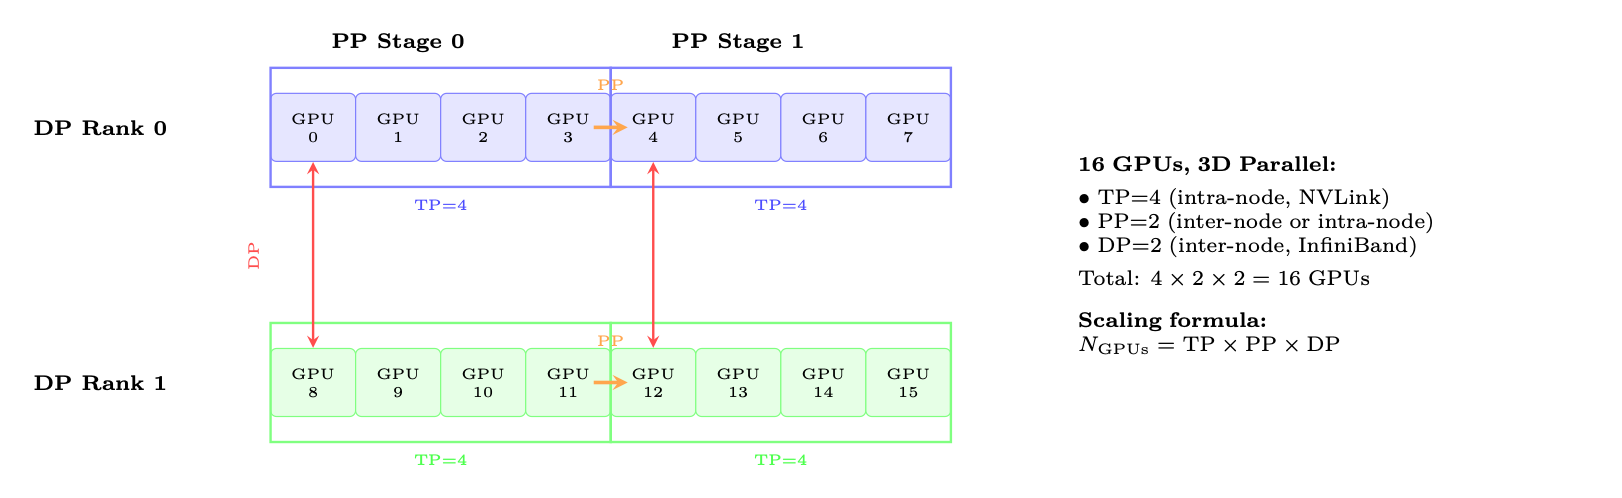
\includegraphics[width=0.95\textwidth]{figures/fig_039_3d-parallel.png}
\caption{3D parallelism layout for 16 GPUs: TP=4 (within each box, using NVLink), PP=2 (orange arrows, stages), DP=2 (red arrows, gradient sync). Each dimension exploits a different level of the communication hierarchy.}
\label{fig:3d-parallel}
\end{figure}

\begin{keybox}[Production Recipe: 70B on 64 A100-80GB (8 nodes)]
\textbf{Intra-node} (NVLink 600GB/s): TP=8 for generation, FSDP within node for training.\\

\textbf{Inter-node} (InfiniBand 400Gb/s): FSDP across nodes (8-way data parallel).\\

\textbf{Result}: Each GPU holds $\sim$70GB. Policy weights gathered per-layer during forward/backward.\\

\textbf{Pipeline Parallel}: Only if model exceeds 100B+ and won’t fit with TP+ZeRO. Adds complexity (bubble overhead 10--20\%) and scheduling headaches.

\textbf{Decision flowchart}:

\begin{enumerate}
  \item Does the model fit on 1 GPU? $\rightarrow$ Use DDP.
  \item Does it fit on 1 node with FSDP? $\rightarrow$ Use FSDP (ZeRO-3).
  \item Does it fit on 1 node with TP+FSDP? $\rightarrow$ Use TP (intra-node) + FSDP (inter-node).
  \item Still doesn’t fit? $\rightarrow$ Add PP across nodes. This is the last resort.
\end{enumerate}
\end{keybox}

\begin{table}[ht!]
\centering
\caption{Parallelism strategy comparison summary}
{\footnotesize
\begin{tabular}{@{}llllll@{}}
\toprule
\textbf{Strategy} & \textbf{Splits} & \textbf{Communication} & \textbf{Scaling Limit} & \textbf{Overhead} & \textbf{When to Use} \\
\midrule
DP/DDP & Batch & AllReduce (grads) & $\sim$64 GPUs & 5--10\% & Model fits on 1 GPU \\
FSDP & Params+Opt+Grad & AllGather+RS & 100s of GPUs & 10--20\% & Default for $>$13B \\
TP & Weight matrices & AllReduce (2/layer) & 8 GPUs (1 node) & 12--18\% & Large model inference+train \\
SP & Activations (seq) & Reuses TP comms & Same as TP & $\approx$0\% extra & Always with TP \\
PP & Layers (stages) & Point-to-point & $\sim$16 stages & 15--30\% & 100B+ models only \\
\bottomrule
\end{tabular}
}
\end{table}

\section{The Generation Bottleneck: Quantitative Analysis}
\label{the-generation-bottleneck-quantitative-analysis}

\begin{intuitionbox}[Roofline Analysis: Why Generation is Memory-Bound]
\textbf{A100 specs}: 312 TFLOPS (BF16 tensor cores), 2 TB/s HBM bandwidth.

\textbf{Roofline crossover}: $312\text{T} / 2\text{T} = 156$ FLOP/byte. Operations below 156 FLOP/byte are \emph{memory-bound}.

\textbf{Autoregressive generation}: For each token, read all weights (140GB for 70B) and do $2 \times 70\text{B} = 140\text{G}$ FLOPs per token (at batch=1).

\textbf{Arithmetic intensity}: $140\text{G FLOP} / 140\text{GB} = 1$ FLOP/byte. That’s $156\times$ below the roofline!

\textbf{Utilization}: $1/156 = 0.6\%$ of peak FLOPS utilized. The GPU is 99.4\% idle, waiting for memory reads.

\textbf{Token rate}: $2\text{TB/s} / 140\text{GB} = 14.3$ tokens/second (single stream, batch=1).

\textbf{For 512 tokens}: $512 / 14.3 = 35.8$ seconds per response (batch=1, TP=1).

\textbf{Batching helps}: Batch=64 with TP=4 $\rightarrow$ reads weights once, generates 64 tokens in parallel. Arithmetic intensity: $64 \times 1 = 64$ FLOP/byte. Better, but still below roofline!
\end{intuitionbox}

\begin{table}[ht!]
\centering
\caption{Generation throughput for 70B model (512 tokens, various configurations)}
{\footnotesize
\begin{tabular}{@{}lllll@{}}
\toprule
\textbf{Config} & \textbf{Batch} & \textbf{Time/batch} & \textbf{Tok/s/GPU} & \textbf{Notes} \\
\midrule
TP=1, batch=1 & 1 & 36s & 14 & Baseline, worst case \\
TP=4, batch=1 & 1 & 9s & 57 & Linear TP scaling for gen \\
TP=4, batch=32 & 32 & 15s & 1092 & Near-optimal batching \\
TP=4, batch=128, vLLM & 128 & 45s & 1456 & Continuous batching \\
TP=4, batch=128, INT8 & 128 & 25s & 2621 & 2$\times$ bandwidth savings \\
\bottomrule
\end{tabular}
}
\end{table}

\textbf{Optimization stack} (cumulative speedup):

\begin{enumerate}
  \item \textbf{vLLM + PagedAttention}~\cite{kwon2023efficient} (2--4$\times$): Eliminates KV cache fragmentation, enables larger batches
  \item \textbf{Continuous batching}~\cite{yu2022orca} (1.5--2$\times$): Don’t wait for longest sequence; start new ones as others finish
  \item \textbf{Speculative decoding}~\cite{leviathan2023fast} (2--3$\times$): Small draft model proposes 5 tokens, large model verifies in one forward pass. Accept 3--4 on average.
  \item \textbf{INT8/FP8 weights for gen} (2$\times$): Halve bandwidth needs. Quality loss is minimal since we’re sampling (not computing exact logits for training)
  \item \textbf{CUDA graphs} (1.1--1.3$\times$): Eliminate kernel launch overhead for fixed-shape operations
  \item \textbf{Prefix caching} (1.5$\times$ for shared-prefix prompts): Don’t recompute system prompt KV cache
\end{enumerate}

\begin{lstlisting}[style=pythonstyle]
# Production vLLM generation setup
from vllm import LLM, SamplingParams

engine = LLM(
    model="./policy_checkpoint",
    tensor_parallel_size=4,           # TP=4 per instance
    gpu_memory_utilization=0.92,      # Leave headroom for KV cache
    max_num_batched_tokens=16384,     # Max tokens in flight
    max_num_seqs=256,                 # Max concurrent sequences
    dtype="bfloat16",
    enable_prefix_caching=True,       # Cache system prompt KV
    speculative_model="./draft_1B",   # Speculative decoding
    num_speculative_tokens=5,
    block_size=16,                    # PagedAttention block size
    swap_space=4,                     # GB swap space for preemption
)

# Generate responses for RLHF batch
sampling_params = SamplingParams(
    temperature=0.7, top_p=0.9, max_tokens=512,
    logprobs=1,  # Need log-probs for PPO ratio calculation
)
outputs = engine.generate(prompts, sampling_params)
# Extract: responses, log_probs for each token (needed for PPO/GRPO)
\end{lstlisting}

\section{Decoupled Architecture: Production Design}
\label{decoupled-architecture-production-design}

Production RLHF systems such as DeepSpeed-Chat~\cite{yao2023deepspeedchat} and OpenRLHF~\cite{hu2024openrlhf} use a \textbf{decoupled architecture} that separates generation, scoring, and training into independently scalable clusters.

\begin{figure}[ht!]
\centering
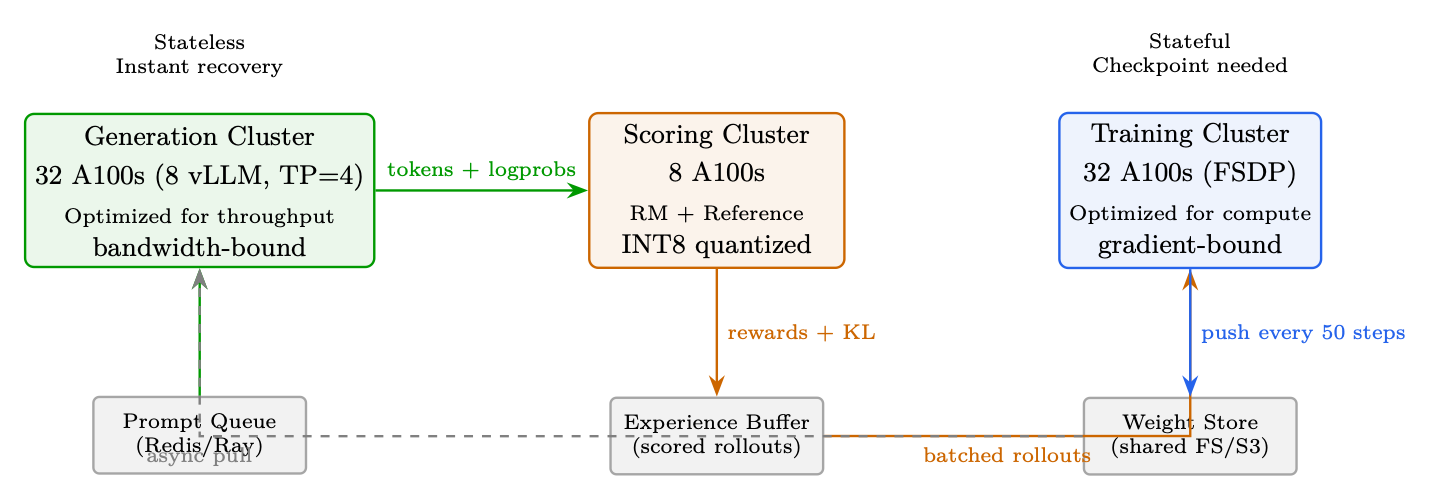
\includegraphics[width=0.85\textwidth]{figures/fig_040_fig40.png}
\caption{Decoupled RLHF architecture. Each cluster optimized for its workload. Scored rollouts accumulate in the experience buffer before being consumed by training.}
\end{figure}

\begin{keybox}[Why Decouple?]
\textbf{Generation} is memory-bandwidth bound (need fast HBM, waste compute).\\

\textbf{Training} is compute-bound (need tensor cores, waste bandwidth during backprop).\\

\textbf{Same hardware can’t optimize both}: If you put everything together, you either waste compute during generation or waste bandwidth during training. Decoupling lets each cluster use optimal hardware/config.

\textbf{Practical benefits}:

\begin{itemize}
  \item Scale generation and training independently
  \item Generation cluster is stateless $\rightarrow$ trivial fault tolerance
  \item Can overlap gen(step $N+1$) with training(step $N$) $\rightarrow$ 30--40\% speedup
  \item Different quantization: INT8 for generation (bandwidth), BF16 for training (precision)
\end{itemize}
\end{keybox}

\section{Weight Synchronization Strategies}
\label{weight-synchronization-strategies}

{\small
\begin{tabular}{@{}llll@{}}
\toprule
\textbf{Strategy} & \textbf{Staleness} & \textbf{Bandwidth} & \textbf{Quality Impact} \\
\midrule
Synchronous (every step) & 0 steps & 140 GB/step & Perfect but too slow \\
Periodic (every 50 steps) & 25 avg & 2.8 GB/step amortized & $<$2\% quality loss \\
Delta compression (INT8) & 25 avg & 0.4 GB/step & $<$3\% quality loss \\
Async streaming & 5--10 steps & 14 GB/step (background) & $<$1\% quality loss \\
\bottomrule
\end{tabular}
}

\begin{intuitionbox}[Why Staleness is OK for PPO/GRPO]
PPO’s clipped objective was \emph{designed} for off-policy data! The clip $[1-\epsilon, 1+\epsilon]$ bounds the impact of stale data. With 10--50 steps of staleness:

\begin{itemize}
  \item Policy changes $\sim$0.1--1\% per step (with proper LR)
  \item Over 50 steps: $\sim$5\% policy drift
  \item PPO clip handles up to 20\% drift by design
  \item Empirically: quality loss $<$2\% for 50-step staleness
\end{itemize}

\textbf{Bandwidth math}: 70B BF16 = 140GB. InfiniBand 400Gb/s = 50GB/s $\rightarrow$ full sync in 2.8s. With delta compression: $<$0.5s. Async = free (runs in background).
\end{intuitionbox}

\section{Memory Optimization Techniques}
\label{memory-optimization-techniques}

\begin{tabular}{@{}lp{5cm}p{8cm}@{}}
\toprule
\textbf{ZeRO Stage} & \textbf{What Gets Sharded} & \textbf{Memory/GPU (70B, 8 GPUs)} \\
\midrule
None (Data Parallel) & Nothing (full replica) & 560GB per GPU (impossible) \\
ZeRO-1 & Optimizer states only & 175GB \\
ZeRO-2 & Optimizer states + Gradients & 105GB \\
ZeRO-3 (FSDP) & Optimizer + Gradients + Parameters & \textbf{70GB (fits in A100-80GB!)} \\
\bottomrule
\end{tabular}

\textbf{Additional techniques}:

\begin{itemize}
  \item \textbf{Gradient checkpointing}~\cite{chen2016training}: Don’t store all activations; recompute during backward pass. Saves $\sim$60\% activation memory, costs $\sim$33\% extra compute. Selective: only checkpoint attention layers (memory-heavy), keep FFN activations (compute-heavy to recompute).
  \item \textbf{Mixed precision}~\cite{micikevicius2018mixed}: Forward in BF16 (2 bytes/param), optimizer states in FP32 (4 bytes each for m,v). Master weights in FP32 for accumulation.
  \item \textbf{CPU offloading} (ZeRO-Infinity~\cite{rajbhandari2021zeroinfinity}): Move optimizer states to CPU RAM. 50\% memory savings but 2--3$\times$ slower (PCIe 64GB/s bottleneck).
  \item \textbf{Activation offloading}: Move activations to CPU during forward, bring back for backward. Only when memory is truly critical.
  \item \textbf{Flash Attention}~\cite{dao2022flashattention, dao2023flashattention2}: O($n$) memory instead of O($n^2$) for attention. 2--4$\times$ faster + massive memory savings for long sequences.
\end{itemize}

\subsection{Flash Attention’s Impact on RLHF}
\label{flash-attentions-impact-on-rlhf}

\begin{intuitionbox}[Why Flash Attention Matters for RLHF]
RLHF involves generating long sequences (rollouts) and then training on them. Without Flash Attention:

\begin{itemize}
  \item A 4K-token sequence with 32 heads requires $\sim$4 GB just for attention matrices
  \item This severely limits batch size during PPO/GRPO training
  \item Gradient checkpointing of attention activations is expensive
\end{itemize}

With Flash Attention:

\begin{itemize}
  \item Attention memory is $O(n)$ -- dominated by $Q, K, V, O$ tensors
  \item Longer rollouts (8K--32K tokens) become feasible with the same GPU memory
  \item Backward pass recomputes attention tiles from $Q, K, V$ (no stored $n^2$ matrix)
  \item This is the key enabler for long-context RLHF (e.g., reasoning models)
\end{itemize}
\end{intuitionbox}

\begin{warningbox}[Flash Attention and Gradient Checkpointing]
Flash Attention’s backward pass recomputes the attention tiles on-the-fly from $Q, K, V$ (which are stored). This means Flash Attention \emph{already implements} a form of activation recomputation for the $O(n^2)$ attention matrix. You do not need to additionally checkpoint the attention layer -- doing so would recompute $Q, K, V$ unnecessarily.
\end{warningbox}

\begin{lstlisting}[style=pythonstyle]
# DeepSpeed ZeRO-3 configuration for 70B RLHF training
ds_config = {
    "bf16": {"enabled": True},
    "zero_optimization": {
        "stage": 3,
        "overlap_comm": True,                    # Overlap communication with compute
        "contiguous_gradients": True,            # Better memory layout
        "reduce_scatter": True,                  # More efficient than allreduce
        "reduce_bucket_size": 5e7,               # 50M params per bucket
        "prefetch_bucket_size": 5e7,             # Prefetch next bucket
        "param_persistence_threshold": 1e5,      # Keep small params on all GPUs
        "offload_optimizer": {"device": "cpu", "pin_memory": True},  # CPU offload
        "sub_group_size": 1e9,                   # Reduce fragmentation
    },
    "gradient_accumulation_steps": 4,
    "gradient_clipping": 1.0,
    "train_micro_batch_size_per_gpu": 2,
    "wall_clock_breakdown": True,
}
\end{lstlisting}

\section{Fault Tolerance at Scale}
\label{fault-tolerance-at-scale}

\begin{warningbox}[Hardware Failure Reality]
\textbf{Individual GPU MTBF}: $\sim$10,000 hours.\\
\textbf{512-GPU cluster MTBF}: $10000/512 \approx 20$ hours. But with software/network: \textbf{4--8 hours realistically}.\\
\textbf{Multi-day training run}: Will see 5--15 failures. Without fault tolerance, one failure kills everything.
\end{warningbox}

\textbf{Production fault tolerance stack}:

\begin{enumerate}
  \item \textbf{Detection}: NCCL timeout (60s), GPU heartbeat (10s), NVML health monitoring, ECC error counting.
  \item \textbf{Checkpointing}: Async every 50--100 steps. Non-blocking (background thread). Save: model weights, optimizer states (Adam m/v), scheduler state, RNG states, KL coefficient, replay buffer. Keep last 3 checkpoints. Time: $\sim$30s for 70B (parallel write to NVMe).
  \item \textbf{Recovery}: (a) Generation cluster = stateless, just restart and load latest weights. (b) Training cluster: load checkpoint, rebuild NCCL process group excluding failed node, redistribute FSDP shards, resume from last checkpoint.
  \item \textbf{Elastic training}: Torch Elastic / Kubernetes auto-scaling. Replace failed node within minutes. Training continues with $N-1$ GPUs temporarily.
  \item \textbf{Prevention}: GPU health pre-screening (run GEMM stress test before starting). Hot spares on standby. Redundant network paths (dual-rail InfiniBand).
\end{enumerate}

\section{End-to-End Latency Breakdown}
\label{end-to-end-latency-breakdown}

\begin{figure}[ht!]
\centering
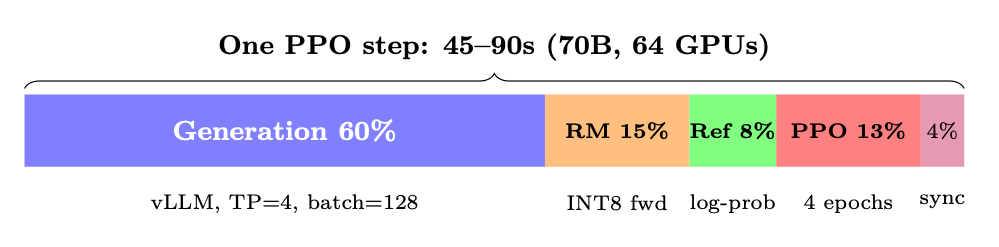
\includegraphics[width=0.85\textwidth]{figures/fig_041_fig41.png}
\caption{Without overlap (monolithic). With decoupled: gen overlaps with training, effective 1.4$\times$ speedup.}
\end{figure}

\begin{tabular}{@{}lp{3.5cm}p{3.5cm}p{6cm}@{}}
\toprule
\textbf{Phase} & \textbf{Time (70B)} & \textbf{Bound By} & \textbf{Optimization} \\
\midrule
Generation (128$\times$512 tok) & 30--45s & Memory bandwidth & vLLM, spec decoding, INT8 \\
Reward scoring & 5--8s & Compute (batch forward) & INT8 RM, batch=128 \\
Reference log-probs & 4--6s & Compute (batch forward) & INT8 ref, or LoRA (free) \\
PPO update (4 epochs) & 8--12s & Compute (backprop) & FSDP, Flash Attention \\
Weight sync & 0--3s & Network (async) & Delta compression, async \\
\textbf{Total (monolithic)} & \textbf{50--75s} &  &  \\
\textbf{Total (decoupled, overlapped)} & \textbf{35--50s} &  & Gen overlaps with prev training \\
\bottomrule
\end{tabular}

\section{Monitoring and Observability}
\label{monitoring-and-observability}

\begin{keybox}[Key Metrics to Track During RLHF Training]
\textbf{Quality metrics} (log every 10 steps):

\begin{itemize}
  \item Mean reward (should increase then plateau)
  \item KL divergence from reference (should stay 3--10)
  \item Response length distribution (watch for length hacking)
  \item Entropy (should decrease slowly, not collapse)
\end{itemize}

\textbf{System metrics} (log every step):

\begin{itemize}
  \item GPU utilization (target: $>$80\% during training, $>$60\% during gen)
  \item Memory watermark per GPU (catch OOM before it happens)
  \item Generation throughput (tokens/sec, should be stable)
  \item Gradient norm (spikes = instability incoming)
  \item NCCL communication time (detect network degradation)
\end{itemize}
\end{keybox}

\section{Network Topology and Communication Patterns}
\label{sec:network-topology}

Efficient distributed training requires understanding the hierarchical communication fabric that connects GPUs. Modern clusters use a two-tier architecture: ultra-fast intra-node links and slower but scalable inter-node networks.

\subsection{Intra-Node: NVLink and NVSwitch}
\label{intra-node-nvlink-and-nvswitch}

\begin{table}[ht!]
\centering
\caption{NVLink generations and their impact on LLM training}
\begin{tabular}{@{}lp{3cm}p{3.2cm}p{3.2cm}p{3.5cm}@{}}
\toprule
\textbf{Generation} & \textbf{BW per link} & \textbf{Links/GPU} & \textbf{Total BW} & \textbf{Platform} \\
\midrule
NVLink 3.0 & 50 GB/s & 12 & 600 GB/s & A100 (DGX A100) \\
NVLink 4.0 & 50 GB/s & 18 & 900 GB/s & H100 (DGX H100) \\
NVLink 5.0 & 100 GB/s & 18 & 1800 GB/s & B200 (DGX B200) \\
\bottomrule
\end{tabular}
\end{table}

Within a single node (typically 8 GPUs), \textbf{NVSwitch} provides full-bisection bandwidth between all GPU pairs. This means any GPU can communicate with any other at full NVLink speed simultaneously---critical for Tensor Parallelism where every layer requires an AllReduce across all 8 GPUs.

\begin{keybox}[NVSwitch vs PCIe Topology]
\textbf{With NVSwitch} (DGX/HGX): All 8 GPUs connected all-to-all at 600--1800~GB/s. AllReduce for TP takes $\sim$0.2ms per layer.

\textbf{Without NVSwitch} (PCIe-only servers): GPUs communicate through CPU PCIe root complex at 32--64~GB/s. TP across 8 GPUs becomes 10--30$\times$ slower. \textbf{Never use TP$>$2 on PCIe-only systems.}
\end{keybox}

\subsection{Inter-Node: InfiniBand and RoCE}
\label{inter-node-infiniband-and-roce}

For FSDP/ZeRO-3 AllGather and ReduceScatter operations across nodes, the inter-node network dominates.

\begin{table}[ht!]
\centering
\caption{Inter-node networking options for LLM training clusters}
{\small
\begin{tabular}{@{}llll@{}}
\toprule
\textbf{Technology} & \textbf{Bandwidth} & \textbf{Latency} & \textbf{Notes} \\
\midrule
InfiniBand NDR & 400 Gb/s (50 GB/s) & 1--2 $\mu$s & Gold standard, RDMA, lossless \\
InfiniBand NDR (dual-rail) & 800 Gb/s (100 GB/s) & 1--2 $\mu$s & Used in H100 clusters \\
RoCE v2 & 100--400 Gb/s & 2--5 $\mu$s & Cheaper, needs PFC/ECN tuning \\
Ethernet (TCP) & 100--400 Gb/s & 10--50 $\mu$s & Not suitable for $>$16 GPU training \\
\bottomrule
\end{tabular}
}
\end{table}

\subsection{Communication Primitives and Their Costs}
\label{communication-primitives-and-their-costs}

Understanding when each collective is used helps diagnose bottlenecks:

\begin{table}[ht!]
\centering
\caption{NCCL collective operations in distributed LLM training}
\begin{tabular}{@{}lp{3.5cm}p{3.5cm}p{6cm}@{}}
\toprule
\textbf{Collective} & \textbf{Data Moved} & \textbf{Used By} & \textbf{When} \\
\midrule
AllReduce & $2 \cdot \frac{N-1}{N} \cdot M$ & TP, DP & Sum gradients or activations across GPUs \\
AllGather & $\frac{N-1}{N} \cdot M$ & FSDP forward & Reconstruct full parameter tensor before matmul \\
ReduceScatter & $\frac{N-1}{N} \cdot M$ & FSDP backward & Distribute gradient shards after backprop \\
Broadcast & $M$ & PP & Send activations to next pipeline stage \\
Send/Recv & $M$ & PP & Point-to-point between adjacent stages \\
\bottomrule
\end{tabular}
\end{table}

where $M$ is the message size (bytes) and $N$ is the number of participants.

\newpage
\begin{intuitionbox}[Communication-Computation Overlap]
Modern frameworks (FSDP, DeepSpeed) aggressively overlap communication with computation:

\textbf{Forward pass}: While layer $i$ computes, AllGather prefetches parameters for layer $i+1$. After layer $i$ finishes, its parameters are immediately discarded (``free-after-forward'').

\textbf{Backward pass}: While layer $i$ computes gradients, ReduceScatter sends layer $i+1$’s gradients. This overlap hides 70--90\% of communication latency when properly tuned.

\textbf{Tuning knobs}: \texttt{prefetch\_factor} (how many layers ahead to prefetch), \texttt{reduce\_bucket\_size} (granularity of gradient reduction), \texttt{backward\_prefetch} (``pre'' vs ``post'' backward prefetch strategy).
\end{intuitionbox}

\subsection{Network Topology Design}
\label{network-topology-design}

Production clusters use \textbf{fat-tree} or \textbf{rail-optimized} topologies:

\begin{itemize}
  \item \textbf{Fat-tree}: Full bisection bandwidth at every level. Any node can communicate with any other at full speed. Expensive (many switches) but maximally flexible.
  \item \textbf{Rail-optimized}: GPU $i$ on every node connects to the same leaf switch (``rail $i$''). AllReduce within a rail is cheap; cross-rail traffic is expensive. Used by Meta’s RSC and Google’s TPU pods.
  \item \textbf{3D torus / Dragonfly}: Used in HPC clusters (Frontier, Aurora). Topology-aware job placement is critical.
\end{itemize}

\begin{warningbox}[Job Placement Matters]
On a 512-GPU cluster, random node assignment can cause 2--3$\times$ slowdown due to network congestion. \textbf{Always request contiguous node blocks.} Production schedulers (Slurm, Kubernetes) should enforce locality: all nodes in a training job should be on the same leaf switch or within one hop of each other.
\end{warningbox}

\section{Training Throughput and Model FLOPs Utilization}
\label{sec:mfu}

\subsection{Measuring Training Efficiency: MFU}
\label{measuring-training-efficiency-mfu}

\textbf{Model FLOPs Utilization (MFU)}~\cite{chowdhery2022palm} is the standard metric for training efficiency:

\begin{equation}
\text{MFU} = \frac{\text{Observed throughput (tokens/sec)} \times \text{FLOPs per token}}{\text{Peak hardware FLOPS}}
\end{equation}

For a transformer with $P$ parameters, $s$ sequence length, and $b$ batch size: 
\begin{equation}
\text{FLOPs per token} \approx 6P + 12 \cdot n_\text{layers} \cdot d_\text{model} \cdot s
\end{equation}

The factor of 6 comes from: 2 (multiply-add) $\times$ 3 (forward + backward, where backward $\approx 2\times$ forward). The second term accounts for attention’s $O(s^2)$ cost.

\begin{table}[ht!]
\centering
\caption{MFU benchmarks across scales and hardware}
\begin{tabular}{@{}lp{3cm}p{3.2cm}p{3.2cm}p{3.5cm}@{}}
\toprule
\textbf{Model} & \textbf{Hardware} & \textbf{MFU} & \textbf{Tokens/sec/GPU} & \textbf{Configuration} \\
\midrule
LLaMA-7B & 8$\times$A100 & 57\% & 3,200 & FSDP, FlashAttn, BF16 \\
LLaMA-13B & 16$\times$A100 & 52\% & 1,750 & FSDP, FlashAttn, BF16 \\
LLaMA-70B & 64$\times$A100 & 45\% & 380 & FSDP+TP=8, FlashAttn \\
GPT-4 (est.) & 10,000+ H100 & 40--50\% & --- & 3D parallelism \\
PaLM-540B & 6144 TPUv4 & 46\% & --- & DP+TP+PP \\
\bottomrule
\end{tabular}
\end{table}

\begin{intuitionbox}[Why MFU Decreases with Scale]
Larger models require more parallelism, which introduces:

\begin{enumerate}
  \item \textbf{Communication overhead}: AllGather/ReduceScatter for FSDP ($\sim$10--15\% at 64 GPUs)
  \item \textbf{Pipeline bubbles}: PP introduces idle time at start/end of micro-batches ($\sim$15--25\% with PP=4)
  \item \textbf{Memory for auxiliary models}: Reference/RM take GPU memory that could hold larger batches
  \item \textbf{Load imbalance}: Not all layers have equal compute (embeddings vs transformer blocks)
\end{enumerate}

\textbf{Rule of thumb}: Target MFU $>$ 40\% for training. If below 30\%, diagnose with profiling.
\end{intuitionbox}

\subsection{Compute-Optimal Batch Sizing}
\label{compute-optimal-batch-sizing}

The effective batch size interacts with hardware utilization in non-obvious ways:

\begin{equation}
\text{Effective batch size} = \text{micro\_batch} \times \text{grad\_accum} \times \text{DP degree}
\end{equation}

\begin{itemize}
  \item \textbf{Too small}: GPU underutilized (low arithmetic intensity), communication dominates.
  \item \textbf{Too large}: Diminishing learning per token (critical batch size exceeded), wastes compute.
  \item \textbf{Sweet spot}: The \emph{critical batch size} $B_\text{crit}$ where gradient noise equals gradient signal. For LLMs, $B_\text{crit} \sim 1$--$4$M tokens~\cite{mccandlish2018empirical}.
\end{itemize}

For RLHF specifically, the batch contains \emph{rollouts} (not just tokens): 
\begin{equation}
\text{RLHF batch} = N_\text{prompts} \times K_\text{generations} \times L_\text{avg response length}
\end{equation}

Typical production values: $N=128$ prompts, $K=1$--$4$ generations, $L=256$--$512$ tokens $\rightarrow$ 32K--256K tokens per step.

\subsection{Profiling and Bottleneck Diagnosis}
\label{profiling-and-bottleneck-diagnosis}

Key profiling tools and what they reveal:

\begin{tabular}{@{}lp{5cm}p{8cm}@{}}
\toprule
\textbf{Tool} & \textbf{Captures} & \textbf{Best For} \\
\midrule
\texttt{torch.profiler} & Kernel timing, memory & Finding slow ops, memory leaks \\
NVIDIA Nsight Systems & Full GPU timeline & Visualizing overlap, gaps between kernels \\
\texttt{nccl\_debug=INFO} & Collective sizes/times & Diagnosing communication bottlenecks \\
\texttt{torch.cuda.memory\_stats} & Allocation patterns & Finding fragmentation, peak usage \\
DeepSpeed Flops Profiler & Per-layer FLOPs & Identifying load imbalance \\
\texttt{py-spy} / \texttt{scalene} & CPU profiling & Data loading, tokenization bottlenecks \\
\bottomrule
\end{tabular}

\begin{examplebox}[Diagnosing Low MFU: A Checklist]
\begin{enumerate}
  \item \textbf{GPU utilization $<$ 80\%?} $\rightarrow$ Data loading bottleneck (check CPU, I/O).
  \item \textbf{Large gaps between kernels?} $\rightarrow$ Python overhead, synchronization points. Use CUDA graphs.
  \item \textbf{Communication $>$ 20\% of step time?} $\rightarrow$ Reduce TP degree, increase batch size, check network health.
  \item \textbf{Memory at 99\%?} $\rightarrow$ Cannot increase batch. Try gradient checkpointing, offloading.
  \item \textbf{OOM during generation?} $\rightarrow$ KV cache too large. Reduce max\_seq\_len or batch size for gen.
\end{enumerate}
\end{examplebox}

\section{Cost Analysis and Cloud Deployment}
\label{cost-analysis-and-cloud-deployment}

Understanding the economics of RLHF training is essential for planning.

\subsection{Hardware Cost Comparison}
\label{hardware-cost-comparison}

\begin{table}[ht!]
\centering
\caption{Approximate cloud GPU costs for RLHF training (2024--2025 pricing)}
\begin{tabular}{@{}lp{3cm}p{3.2cm}p{3.2cm}p{3.5cm}@{}}
\toprule
\textbf{GPU} & \textbf{On-Demand/hr} & \textbf{Spot/hr} & \textbf{Memory} & \textbf{Use Case} \\
\midrule
A100 80GB & \$2.50--3.50 & \$1.00--1.50 & 80 GB HBM2e & Budget training, gen cluster \\
H100 80GB & \$4.00--6.00 & \$2.00--3.00 & 80 GB HBM3 & Production training \\
H200 141GB & \$6.00--8.00 & --- & 141 GB HBM3e & Large context, fewer-GPU configs \\
MI300X 192GB & \$3.50--5.00 & \$1.50--2.50 & 192 GB HBM3 & Cost-effective alternative \\
\bottomrule
\end{tabular}
\end{table}

\subsection{RLHF Training Cost Estimation}
\label{rlhf-training-cost-estimation}

\begin{equation}
\text{Cost} = \frac{N_\text{steps} \times T_\text{step}}{3600} \times N_\text{GPUs} \times C_\text{GPU/hr}
\end{equation}

\begin{examplebox}[Cost Example: 70B Model RLHF (10K steps)]
\begin{tabular}{@{}lp{11cm}@{}}
\toprule
Steps & 10,000 \\
\midrule
Time per step (decoupled) & 45 seconds \\
Total training time & $10000 \times 45 / 3600 = 125$ hours \\
GPUs (generation + training) & 64 A100-80GB \\
Cost per GPU-hour (spot) & \$1.20 \\
\textbf{Total cost} & $125 \times 64 \times \$1.20 =$ \textbf{\$9,600} \\
\bottomrule
\end{tabular}

\textbf{Breakdown by phase}:

\begin{itemize}
  \item Generation cluster (32 GPUs): \$4,800 (60\% of time)
  \item Training cluster (32 GPUs): \$4,800 (could overlap $\rightarrow$ \$3,400 effective)
  \item Scoring (shared with gen GPUs): included above
\end{itemize}

\textbf{With overlap}: Effective cost $\approx$ \textbf{\$7,500} for full RLHF alignment of a 70B model.
\end{examplebox}

\subsection{Cost Optimization Strategies}
\label{cost-optimization-strategies}

\begin{itemize}
  \item \textbf{Spot/preemptible instances}: 50--70\% savings. Requires robust checkpointing (save every 5 minutes).
  \item \textbf{Right-sizing}: Don’t use H100 for generation (memory-bound); A100 achieves similar tokens/\$ for inference.
  \item \textbf{Quantized inference}: INT8/FP8 for generation and scoring halves GPU count for those clusters.
  \item \textbf{Progressive training}: Start with 8B proxy model for reward engineering/debugging ($\sim$\$200), then scale to 70B.
  \item \textbf{LoRA for reference-free}: Eliminates reference model entirely (50\% memory reduction).
  \item \textbf{Shorter sequences first}: Curriculum from 256$\rightarrow$512$\rightarrow$1024 token generations saves 40\% compute.
\end{itemize}

\section{Distributed Checkpointing}
\label{sec:checkpointing}

At scale, naive checkpointing becomes a bottleneck. A 70B model with optimizer state requires saving $\sim$840~GB per checkpoint (FP32 master weights + Adam m + v).

\subsection{Checkpointing Strategies}
\label{checkpointing-strategies}

\begin{table}[ht!]
\centering
\caption{Checkpointing approaches for large-scale RLHF}
\begin{tabular}{@{}lp{3.5cm}p{3.5cm}p{6cm}@{}}
\toprule
\textbf{Strategy} & \textbf{Save Time (70B)} & \textbf{Storage/ckpt} & \textbf{Characteristics} \\
\midrule
Synchronous (all ranks) & 30--60s (blocking) & 420 GB & Simple, stalls training \\
Async (background copy) & $<$1s (non-blocking) & 420 GB & Overlaps with next step \\
Incremental (delta) & $<$1s & 5--20 GB & Only save changed params \\
Sharded (FSDP native) & 5--10s & 420 GB sharded & Each rank saves its shard \\
\bottomrule
\end{tabular}
\end{table}

\subsection{Production Checkpointing with torch.distributed.checkpoint}
\label{production-checkpointing-with-torch.distributed.checkpoint}

\begin{lstlisting}[style=pythonstyle]
import torch.distributed.checkpoint as dcp
from torch.distributed.checkpoint.state_dict import get_state_dict, StateDictOptions

# Save: each rank writes its shard in parallel
state_dict = {"model": get_state_dict(model, options=StateDictOptions(full_state_dict=False))}
dcp.save(
    state_dict=state_dict,
    storage_writer=dcp.FileSystemWriter("/mnt/checkpoints/step_5000"),
    planner=dcp.DefaultSavePlanner(),  # Handles FSDP sharding automatically
)

# Async save: non-blocking, runs in background thread
future = dcp.async_save(
    state_dict=state_dict,
    storage_writer=dcp.FileSystemWriter("/mnt/checkpoints/step_5000"),
)
# Training continues immediately; future.result() blocks only if needed
\end{lstlisting}

\begin{keybox}[Checkpoint Hygiene for RLHF]
RLHF checkpoints must capture \emph{more} than standard pre-training:

\begin{itemize}
  \item Policy model weights + optimizer states (standard)
  \item KL coefficient ($\beta$) and its schedule state
  \item Replay buffer contents (for off-policy corrections)
  \item RNG states for all GPUs (reproducibility)
  \item Prompt iterator position (avoid re-processing prompts)
  \item Reward model version tag (for auditability)
  \item Wandb/metrics run ID (for continuous logging)
\end{itemize}
\end{keybox}

\section{Hardware Selection Guide}
\label{sec:hardware-guide}

Choosing the right hardware depends on model size, budget, and training phase.

\begin{table}[ht!]
\centering
\caption{Hardware recommendations by model scale and training phase}
\begin{tabular}{@{}lp{3.5cm}p{3.5cm}p{6cm}@{}}
\toprule
\textbf{Model Size} & \textbf{Training Phase} & \textbf{Recommended} & \textbf{Configuration} \\
\midrule
$\leq$7B & SFT + RLHF & 1--2$\times$ A100 & Single node, no parallelism needed \\
7--13B & SFT + RLHF & 4--8$\times$ A100 & FSDP, optional TP=2 for gen \\
13--34B & SFT + RLHF & 8--16$\times$ A100/H100 & FSDP + TP=4 for gen \\
70B & RLHF (full) & 32--64$\times$ A100/H100 & Decoupled, FSDP + TP=8 \\
70B & RLHF (LoRA) & 8--16$\times$ A100/H100 & No ref model, LoRA adapters \\
$>$100B & RLHF & 128+$\times$ H100 & 3D parallelism (TP+PP+DP) \\
\bottomrule
\end{tabular}
\end{table}

\begin{intuitionbox}[H100 vs A100: When is the Upgrade Worth It?]
H100 provides:

\begin{itemize}
  \item $\sim$1.6$\times$ peak FLOPS (989 vs 624 TFLOPS for BF16 with sparsity; 495 vs 312 without sparsity)
  \item $\sim$2$\times$ memory bandwidth (3.35 vs 2.0 TB/s)
  \item FP8 support (additional 2$\times$ for inference)
  \item NVLink 4.0 (900 vs 600 GB/s)
\end{itemize}

\textbf{For training}: $\sim$1.8--2.2$\times$ faster end-to-end (FP8 support and higher bandwidth amplify the raw FLOPS advantage).

\textbf{For generation}: $\sim$1.7$\times$ faster (bandwidth-bound, so 2$\times$ BW $\approx$ 1.7$\times$ throughput with overhead).

\textbf{Cost-performance}: At 1.5$\times$ the price, H100 is almost always better value for training. For inference-only (generation clusters), A100 at spot pricing can be more cost-effective.
\end{intuitionbox}

\section{Optimizer Configuration for RL Training}
\label{sec:rl-optimizer-config}

RL training (PPO, GRPO, DPO) imposes unique demands on the optimizer compared to pretraining or SFT. The loss landscape is non-stationary (the policy changes what data is generated), gradients are noisier (reward signal variance), and training is more prone to catastrophic forgetting or reward hacking. This section consolidates RL-specific optimizer guidance, using AdamW~\cite{loshchilov2019adamw} as the default optimizer.

\subsection{Why RL Requires Different Optimizer Settings}
\label{why-rl-requires-different-optimizer-settings}

\begin{keybox}[RL vs. SFT Optimization – Key Differences]
\begin{itemize}
  \item \textbf{Non-stationary data distribution}: unlike SFT where the dataset is fixed, RL generates new rollouts each iteration---the data distribution shifts with the policy.
  \item \textbf{High gradient variance}: reward signals are sparse and noisy; gradients have much higher variance than cross-entropy on curated data.
  \item \textbf{Smaller updates required}: the policy must stay close to the reference model (KL constraint), so learning rates are 10--100$\times$ smaller than SFT.
  \item \textbf{No weight decay}: regularization comes from the KL penalty, not weight decay. Adding WD on top can fight the KL constraint.
  \item \textbf{Shorter warmup}: RL starts from a converged SFT checkpoint---the optimizer state needs minimal warmup.
\end{itemize}
\end{keybox}

\subsection{Recommended Hyperparameters by RL Method}
\label{recommended-hyperparameters-by-rl-method}

\begin{table}[ht!]
\centering
\caption{Optimizer settings for RL training phases. All use $\beta_1=0.9$, $\beta_2=0.95$, $\epsilon=10^{-8}$, \texttt{max\_grad\_norm}=1.0, BF16.}
{\footnotesize
\begin{tabular}{@{}llllll@{}}
\toprule
\textbf{Method} & \textbf{Optimizer} & \textbf{LR} & \textbf{WD} & \textbf{Warmup} & \textbf{Schedule} \\
\midrule
DPO & AdamW & $5\text{e-}7$ & 0.0 & 50 steps & Constant or Linear \\
PPO (policy) & AdamW & $1\text{e-}6$ & 0.0 & 20 steps & Constant \\
PPO (critic) & AdamW & $1\text{e-}6$ & 0.0 & 20 steps & Constant \\
GRPO & AdamW & $1\text{e-}6$ & 0.0 & 20 steps & Constant \\
\bottomrule
\end{tabular}
}
\end{table}

\begin{intuitionbox}[Why Constant Schedule for RL?]
Cosine and linear-decay schedules assume a fixed training horizon and monotonically decreasing loss. RL training has neither: reward may plateau, spike, or oscillate unpredictably. A constant LR (after brief warmup) keeps the optimizer responsive throughout training. If you must decay, use a very gentle linear schedule with a high minimum LR ratio ($\geq 0.5$).
\end{intuitionbox}

\subsection{Beta-2 = 0.95 for RL: Faster Adaptation}
\label{beta-2-0.95-for-rl-faster-adaptation}

The default Adam $\beta_2 = 0.999$ gives a very long memory for the second moment ($\sim$1000-step effective window). In RL training, the loss landscape changes rapidly as the policy evolves---the gradient variance from 1000 steps ago is irrelevant. Using $\beta_2 = 0.95$ shortens the window to $\sim$20 steps, making the adaptive learning rate respond quickly to changing gradient statistics.

\begin{warningbox}[When beta2 = 0.95 Hurts]
For very small batch sizes (e.g., batch=1 in online RL), $\beta_2 = 0.95$ can make the second moment estimates too noisy. In this regime, use $\beta_2 = 0.99$ as a compromise, or increase the effective batch size via gradient accumulation.
\end{warningbox}

\subsection{Mixed Precision for RL: FP32 Master Weights Are Critical}
\label{mixed-precision-for-rl-fp32-master-weights-are-critical}

RL training is particularly sensitive to numerical precision:

\begin{itemize}
  \item Gradients are noisier---small updates must accumulate accurately over many steps
  \item Learning rates are very small ($10^{-6}$--$10^{-7}$), making $\Delta\theta \ll \theta$
  \item BF16 mantissa (7 bits $\approx$ 0.8\% relative precision) cannot represent updates of magnitude $10^{-6}$ relative to weights of magnitude $10^{0}$
\end{itemize}

\textbf{Always use FP32 master weights for RL training.} BF16-only training (no FP32 copy) reliably causes reward collapse in PPO/GRPO after 100--500 steps.

\subsection{Gradient Clipping is Critical for RL}
\label{gradient-clipping-is-critical-for-rl}

In PPO and GRPO, the reward signal can be highly variable, especially early in training. A single bad batch can produce gradients with norm $>100$, which would completely destroy the model weights. \texttt{max\_grad\_norm=1.0} is the standard setting. For SFT, clipping is less critical but still recommended.

\begin{warningbox}[Never Disable Gradient Clipping for RL]
Unlike SFT where gradient norms are typically stable (0.1--1.0 range), RL gradients are spiky because: (1)~reward variance propagates through the policy gradient, (2)~rare high-reward trajectories create outsized updates, and (3)~the KL penalty term can produce large gradients when the policy drifts. A single unclipped step with $\|\nabla\| > 50$ can undo hundreds of training steps.
\end{warningbox}

\subsection{Diagnosing RL Training Instability}
\label{diagnosing-rl-training-instability}

\begin{examplebox}[Red Flags and Fixes for RL Optimization]
{\small
\begin{tabular}{@{}lp{9.5cm}@{}}
\toprule
\textbf{Symptom} & \textbf{Likely Cause and Fix} \\
\midrule
Reward improves then collapses & LR too high or KL coefficient too low. Reduce LR by 2--5$\times$ or increase $\beta_\text{KL}$. \\
Gradient norm constantly at clip threshold & Updates too aggressive. Reduce LR (clipping means you’re losing gradient direction info every step). \\
KL divergence explodes ($>$15 nats) & LR too high. Reduce by 10$\times$ or add adaptive KL penalty. \\
Reward stuck at baseline & LR too low, or reward model has low signal. Try 2--5$\times$ higher LR. Check reward model calibration. \\
Loss NaN after 100+ steps & FP32 master weights missing, or grad norm overflow. Enable FP32 master weights; verify BF16 mode. \\
\bottomrule
\end{tabular}
}
\end{examplebox}

\subsection{HuggingFace TRL Configuration for RL}
\label{huggingface-trl-configuration-for-rl}

The TRL library~\cite{vonwerra2022trl} provides production-ready implementations of PPO, DPO, and other RL methods for LLMs.

\begin{lstlisting}[style=pythonstyle, caption={Complete PPO and DPO optimizer configuration using TRL.}]
from trl import PPOConfig, PPOTrainer, DPOConfig, DPOTrainer

# --- PPO Configuration ---
ppo_config = PPOConfig(
    # Optimizer (AdamW with RL-specific settings)
    learning_rate=1e-6,           # 10-100x smaller than SFT
    
    # PPO-specific
    ppo_epochs=4,                 # mini-batch updates per rollout
    mini_batch_size=16,
    batch_size=64,                # rollout batch size
    
    # Gradient control
    max_grad_norm=1.0,
    
    # KL penalty (replaces weight decay as regularizer)
    init_kl_coef=0.2,            # initial KL penalty coefficient
    adap_kl_ctrl=True,           # adaptive KL targeting
    target_kl=6.0,               # target KL divergence
    
    # Mixed precision
    bf16=True,                   # BF16 compute, FP32 master weights
)

ppo_trainer = PPOTrainer(
    model=model,
    ref_model=ref_model,
    config=ppo_config,
    tokenizer=tokenizer,
    dataset=dataset,
)

# --- DPO Configuration ---
dpo_config = DPOConfig(
    output_dir="./dpo_output",
    
    # Optimizer
    learning_rate=5e-7,           # even smaller than PPO
    optim="adamw_torch",
    adam_beta1=0.9,
    adam_beta2=0.95,              # shorter memory for RL
    weight_decay=0.0,            # no WD -- KL provides regularization
    
    # Schedule
    lr_scheduler_type="constant_with_warmup",
    warmup_steps=50,
    
    # Gradient control
    max_grad_norm=1.0,
    
    # DPO-specific
    beta=0.1,                    # KL constraint strength
    loss_type="sigmoid",         # standard DPO loss
    
    # Mixed precision
    bf16=True,
    
    # Training
    num_train_epochs=1,          # DPO typically 1 epoch
    per_device_train_batch_size=4,
    gradient_accumulation_steps=8,
)

dpo_trainer = DPOTrainer(
    model=model,
    ref_model=ref_model,
    args=dpo_config,
    train_dataset=dataset,
    tokenizer=tokenizer,
)
dpo_trainer.train()
\end{lstlisting}

\subsection{MoE Considerations for RL Training}
\label{moe-considerations-for-rl-training}

\begin{intuitionbox}[MoE for RLHF]
Mixture-of-Experts (MoE) models~\cite{fedus2022switch} are increasingly used in RLHF:

\begin{itemize}
  \item \textbf{Advantage}: 3--4$\times$ more capacity at same compute cost. Better for reward models (more capacity to judge).
  \item \textbf{Challenge}: Expert parallelism requires all-to-all communication (tokens routed across GPUs). This conflicts with pipeline parallelism.
  \item \textbf{GRPO with MoE}: Works well since generation cost is dominated by active params (not total params).
  \item \textbf{LoRA for MoE}: Can apply LoRA to router + shared layers only, or to all experts (expensive).
\end{itemize}
\end{intuitionbox}

\begin{intuitionbox}[The RL Optimizer Mantra]
For RL fine-tuning: \textbf{small LR, no weight decay, constant schedule, FP32 master weights, aggressive clipping}. Let the KL penalty handle regularization---the optimizer’s job is just to follow the policy gradient without overshooting.
\end{intuitionbox}

\chapter{LLM Agentic Training}
\label{llm-agentic-training}

\section{Motivation: From Chatbots to Autonomous Agents}
\label{motivation-from-chatbots-to-autonomous-agents}

Modern LLMs are increasingly deployed not just as conversational assistants but as \textbf{autonomous agents} that interact with external tools, APIs, databases, and environments over multiple steps. This shift---from single-turn chatbots to multi-step agents---introduces fundamentally new RL challenges that require rethinking how we train, evaluate, and deploy language models.

\begin{figure}[ht!]
\centering
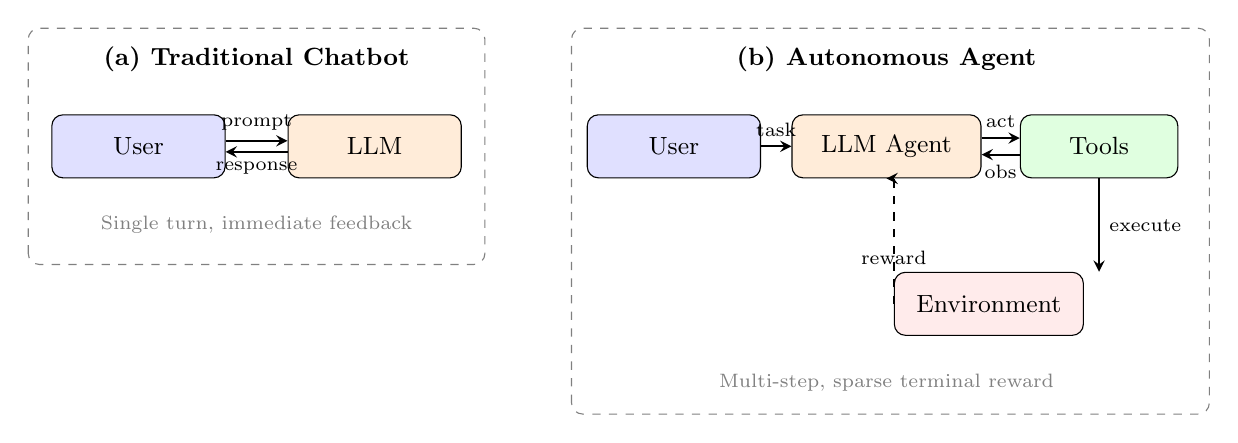
\begin{tikzpicture}[
  box/.style={draw, rounded corners, minimum width=2.2cm, minimum height=0.8cm, font=\small},
  arrow/.style={->, thick, >=stealth},
  lbl/.style={font=\scriptsize, midway, above},
  lblb/.style={font=\scriptsize, midway, below},
]
% --- (a) Chatbot ---
\node[font=\small\bfseries] at (-3.5, 2.6) {(a) Traditional Chatbot};
\node[box, fill=blue!12] (user1) at (-5, 1.5) {User};
\node[box, fill=orange!15] (llm1) at (-2, 1.5) {LLM};
\draw[arrow] ([yshift=2pt]user1.east) -- node[lbl]{prompt} ([yshift=2pt]llm1.west);
\draw[arrow] ([yshift=-2pt]llm1.west) -- node[lblb]{response} ([yshift=-2pt]user1.east);
\node[font=\scriptsize, text=gray] at (-3.5, 0.5) {Single turn, immediate feedback};
\draw[dashed, gray, rounded corners] (-6.4, 0.0) rectangle (-0.6, 3.0);

% --- (b) Autonomous Agent ---
\node[font=\small\bfseries] at (4.5, 2.6) {(b) Autonomous Agent};
\node[box, fill=blue!12] (user2) at (1.8, 1.5) {User};
\node[box, fill=orange!15, minimum width=2.4cm] (agent) at (4.5, 1.5) {LLM Agent};
\node[box, fill=green!12, minimum width=2cm] (tools) at (7.2, 1.5) {Tools};
\node[box, fill=red!8, minimum width=2.4cm] (env) at (5.8, -0.5) {Environment};

% User -> Agent
\draw[arrow] (user2.east) -- node[lbl]{task} (agent.west);
% Agent <-> Tools (bidirectional = the loop)
\draw[arrow] ([yshift=3pt]agent.east) -- node[lbl]{act} ([yshift=3pt]tools.west);
\draw[arrow] ([yshift=-3pt]tools.west) -- node[lblb]{obs} ([yshift=-3pt]agent.east);
% Tools -> Environment
\draw[arrow] (tools.south) -- node[lbl, right]{execute} (tools.south |- env.north);
% Environment -> Agent (reward)
\draw[arrow, dashed] (env.west) -- node[lblb]{reward} (agent.south -| env.west) -- (agent.south);

\node[font=\scriptsize, text=gray] at (4.5, -1.5) {Multi-step, sparse terminal reward};
\draw[dashed, gray, rounded corners] (0.5, -1.9) rectangle (8.6, 3.0);
\end{tikzpicture}
\caption{From Chatbots to Autonomous Agents: Traditional LLM chatbots operate in a single-step conversational loop with immediate human feedback. Autonomous agents plan across multiple tool interactions, receive feedback from real-world execution environments, and optimize for sparse terminal rewards (task success/failure).}
\end{figure}

The key differences that demand new RL approaches:

\begin{itemize}
  \item \textbf{Multi-step reasoning}: Agents must plan across 10--100+ tool calls, not just generate a single response.
  \item \textbf{External environment feedback}: Rewards come from real-world execution (test suites pass, web pages load, code compiles) --- not just human preference scores.
  \item \textbf{Structured actions}: Actions are not just tokens but structured outputs (JSON tool calls, API payloads, code blocks).
  \item \textbf{Long horizons with sparse rewards}: Success/failure may only be determined after many intermediate steps.
\end{itemize}

\begin{intuitionbox}[Why Standard RLHF Falls Short for Agents]
Standard RLHF (PPO/DPO) optimizes for single-turn quality: given a prompt, produce a good response. But agents must:

\begin{itemize}
  \item Decide \emph{when} to use tools vs. reason internally
  \item Recover from errors mid-trajectory (self-correction)
  \item Balance exploration (try new approaches) with exploitation (use known-good patterns)
  \item Handle partial observability (tool outputs may be incomplete or noisy)
\end{itemize}

This requires training methods that reason over \textbf{entire trajectories}, not individual turns.
\end{intuitionbox}

\section{Trajectory Buffers for LLM Agents}
\label{trajectory-buffers-for-llm-agents}

In the context of LLM agents, traditional RL replay buffers undergo a structural transformation. Instead of storing low-dimensional numerical tensors, agentic buffers --- often called \textbf{Trajectory Buffers}, \textbf{Experience Pools}, or \textbf{Memory Banks} --- manage complex textual histories, tool execution outputs, and explicit reasoning steps.

\subsection{Mathematical Structure of an LLM Agent Buffer}
\label{mathematical-structure-of-an-llm-agent-buffer}

In classic RL, a replay buffer stores a flat tuple $(s, a, r, s')$. For an LLM agent, this expands into high-dimensional tokenized text structures:

\begin{equation}
\boxed{e_t = \left( \mathcal{S}_t,\; \mathcal{A}_t,\; \mathcal{R}_t,\; \mathcal{S}_{t+1} \right)}
\end{equation}

\begin{itemize}
  \item $\mathcal{S}_t$: The \textbf{complete context state} --- system prompt, user objective, conversation history, and current environmental variables (e.g., HTML source code, directory structures, database schemas).
  \item $\mathcal{A}_t$: The agent’s \textbf{generated output}, typically composed of a Chain-of-Thought (CoT) reasoning string followed by a structured tool call: 
\begin{equation}
\mathcal{A}_t = \{\text{text}_{\text{reasoning}},\; \text{json}_{\text{tool\_call}}\}
\end{equation}
  \item $\mathcal{R}_t$: \textbf{Evaluation signals} derived from external execution environments (unit test passes, compiler flags, API response codes) or verified by an LLM-as-a-judge system.
  \item $\mathcal{S}_{t+1}$: The \textbf{updated context window}, which appends tool output text or error logs directly into the conversation history.
\end{itemize}

\begin{examplebox}[Concrete Agent Trajectory: Code Debugging]
\textbf{Step 1}: $\mathcal{S}_1$ = ``Fix the failing test in \texttt{utils.py}''\\

$\mathcal{A}_1$ = \emph{``Let me read the file first''} + \texttt{read\_file("utils.py")}\\

$\mathcal{R}_1$ = 0 (intermediate step)\\

\textbf{Step 2}: $\mathcal{S}_2$ = [previous context + file contents]\\

$\mathcal{A}_2$ = \emph{``The bug is on line 42, off-by-one error''} + \texttt{edit\_file("utils.py", ...)}\\

$\mathcal{R}_2$ = 0 (intermediate step)\\

\textbf{Step 3}: $\mathcal{S}_3$ = [previous context + edit confirmation]\\

$\mathcal{A}_3$ = \emph{``Let me verify the fix''} + \texttt{run\_tests()}\\

$\mathcal{R}_3$ = +1.0 (all tests pass --- sparse terminal reward)
\end{examplebox}

\section{Operational Paradigms}
\label{operational-paradigms}

LLM agents leverage specialized trajectory buffers through three primary optimization methodologies:

\subsection{A. Self-Correction and Thought Refinement}
\label{a.-self-correction-and-thought-refinement-star-reflexion}

Two representative methods in this category are STaR \cite{zelikman2022star} and Reflexion \cite{shinn2023reflexion}. When an agent fails a multi-step execution trace, the sub-optimal sequence is saved to the buffer. The framework later samples this trajectory and prompts the LLM to generate an explicit textual critique of its past performance: 
\begin{equation}
\text{Critique} \leftarrow \text{LLM}(\mathcal{S}_{\text{failed}},\; \mathcal{A}_{\text{failed}},\; \mathcal{R}_{=0})
\end{equation}

Once a corrected trajectory achieves a positive reward, it is moved to an optimal experience pool used to update the network weights via fine-tuning (SFT on successful trajectories) or RL (GRPO~\cite{shao2024deepseekmath} with binary pass/fail rewards).

\begin{keybox}[STaR: Self-Taught Reasoner]
\begin{enumerate}
  \item Generate reasoning traces for a batch of problems
  \item Filter: keep only traces that lead to correct answers
  \item Fine-tune the model on successful traces (SFT)
  \item Repeat: the improved model generates better traces in the next iteration
\end{enumerate}

Each iteration bootstraps the model’s reasoning ability using its own successful outputs as training data.
\end{keybox}

\begin{keybox}[Reflexion: Verbal Reinforcement Learning]
\begin{enumerate}
  \item Agent attempts a task, fails
  \item Agent generates a \textbf{verbal reflection}: ``I failed because I didn’t check the return type before calling the API''
  \item Reflection is stored in an episodic memory buffer
  \item On the next attempt, reflections are injected into the prompt as lessons learned
  \item No weight updates needed --- pure in-context learning from self-critique
\end{enumerate}
\end{keybox}

\subsection{B. Off-Policy Exploration}
\label{b.-off-policy-exploration-react-tool-use-frameworks}

This paradigm, exemplified by ReAct \cite{yao2023react} and related tool-use frameworks, involves extensive autonomous exploration. During autonomous exploration (web navigation, database querying, code generation), agents log thousands of exploratory execution paths. The trajectory buffer acts as a filter:

\begin{itemize}
  \item \textbf{Success filtering}: Only trajectories achieving the goal are kept for training.
  \item \textbf{Efficiency ranking}: Among successful traces, prefer the shortest/most efficient tool-use paths.
  \item \textbf{Diversity sampling}: Maintain a diverse set of solution strategies to prevent mode collapse.
\end{itemize}

The optimization algorithm (typically GRPO~\cite{shao2024deepseekmath} or filtered SFT) computes losses exclusively over efficient, successful trajectories while discarding meandering runs.

\subsection{C. Non-Parametric In-Context Learning (RAG over Experiences)}
\label{c.-non-parametric-in-context-learning-rag-over-experiences}

Instead of modifying neural network weights, the trajectory buffer can function as a \textbf{vector database}. Given a new user goal $\mathcal{G}_{\text{new}}$, the system retrieves the most relevant past experiences: 
\begin{equation}
\boxed{\mathcal{E}_{\text{retrieved}} = \arg\max_{e \in \mathcal{B}} \text{sim}\!\left(\text{Embed}(\mathcal{G}_{\text{new}}),\; \text{Embed}(e)\right)}
\end{equation}

The top-$k$ similar successful historical runs are injected directly into the prompt context as few-shot demonstrations. This approach:

\begin{itemize}
  \item Requires \textbf{zero training} --- pure retrieval-augmented generation
  \item Adapts instantly to new tasks if similar experiences exist in the buffer
  \item Scales with buffer size (more experiences = better coverage)
  \item Complements parametric learning (use retrieval for rare cases, weights for common patterns)
\end{itemize}

\section{Paradigm Comparison}
\label{paradigm-comparison}

\begin{table}[ht!]
\centering
\caption{Traditional RL Buffers vs. LLM Agent Buffers}
\begin{tabular}{@{}lp{5cm}p{8cm}@{}}
\toprule
\textbf{Feature} & \textbf{Traditional RL Buffer} & \textbf{LLM Agent Buffer} \\
\midrule
\textbf{Data Format} & Continuous vectors / tensors & Tokenized text, JSON, code blocks, tool outputs \\
\textbf{Data Volume} & Massive ($10^5$--$10^7$ items) & Small to medium ($10^3$--$10^5$ traces) \\
\textbf{Primary Goal} & Breaking data correlation & Providing reasoning demonstrations \\
\textbf{Sampling} & Random uniform / PER & Semantic retrieval / success priority / diversity \\
\textbf{State Size} & Fixed (e.g., 84$\times$84 pixels) & Variable (1K--128K tokens per state) \\
\textbf{Action Space} & Discrete/continuous vectors & Structured text (reasoning + tool calls) \\
\textbf{Reward Source} & Environment simulator & External execution / LLM judge / unit tests \\
\bottomrule
\end{tabular}
\end{table}

\section{Major Techniques in Agentic RL}
\label{major-techniques-in-agentic-rl}

\begin{table}[ht!]
\centering
\caption{Key methods for training LLM agents with RL.}
\begin{tabular}{@{}lp{5cm}p{8cm}@{}}
\toprule
\textbf{Method} & \textbf{Type} & \textbf{Key Idea} \\
\midrule
\textbf{STaR}~\cite{zelikman2022star} & Iterative SFT & Bootstrap reasoning by fine-tuning on own successful traces \\
\textbf{Reflexion}~\cite{shinn2023reflexion} & In-context RL & Verbal self-critique stored as episodic memory; no weight updates \\
\textbf{ReAct}~\cite{yao2023react} & Prompting & Interleave reasoning (``think'') and acting (``tool call'') in a single generation \\
\textbf{LATS}~\cite{zhou2024lats} & Tree search & Monte Carlo Tree Search over action sequences; backpropagate rewards \\
\textbf{AgentQ}~\cite{putta2024agentq} & Off-policy RL & DPO on agent trajectories with AI-generated preference pairs \\
\textbf{OpenHands}~\cite{wang2024openhands} & GRPO & Group-relative optimization with execution-based rewards (tests pass/fail) \\
\textbf{Voyager}~\cite{wang2023voyager} & Skill library & Successful code snippets stored and retrieved for compositional reuse \\
\textbf{RLEF}~\cite{le2024rlef} & Online RL & RL from Execution Feedback --- binary reward from code/test execution \\
\bottomrule
\end{tabular}
\end{table}

\subsection{STaR: Self-Taught Reasoner (Detailed)}
\label{star-self-taught-reasoner-detailed}

STaR~\cite{zelikman2022star} is an \textbf{iterative self-improvement} method that bootstraps reasoning capabilities without external reward models. The core insight: if the model can occasionally solve a problem correctly, it can learn from its own successes.

\textbf{Algorithm}:

\begin{enumerate}
  \item \textbf{Generate}: For each problem $x_i$ in dataset $\mathcal{D}$, sample a reasoning trace $z_i \sim \pi_\theta(\cdot | x_i)$ followed by an answer $\hat{y}_i$.
  \item \textbf{Filter}: Keep only traces where $\hat{y}_i = y_i^*$ (correct answer). Define success set $\mathcal{D}_{\text{pass}} = \{(x_i, z_i, y_i^*) : \hat{y}_i = y_i^*\}$.
  \item \textbf{Rationalization} (key innovation): For problems where the model failed, generate a ``rationalization'' --- a trace conditioned on the correct answer: $z_i^{\text{rat}} \sim \pi_\theta(\cdot | x_i, y_i^*)$. This teaches the model to reason \emph{backward} from solutions.
  \item \textbf{Fine-tune}: Update $\theta$ via SFT on $\mathcal{D}_{\text{pass}} \cup \mathcal{D}_{\text{rationalized}}$.
  \item \textbf{Iterate}: Repeat from step 1 with the improved model.
\end{enumerate}

\begin{equation}
\boxed{\theta_{k+1} = \arg\min_\theta -\sum_{(x,z,y) \in \mathcal{D}_k^+} \log \pi_\theta(z, y | x)}
\end{equation}

\textbf{Convergence dynamics}: Each iteration $k$ increases the model’s solve rate $p_k$. If $p_0 = 0.3$ (solves 30\% of problems), after rationalization + SFT, $p_1 \approx 0.5$. Typically converges in 3--5 iterations to $p \approx 0.7$--$0.9$.

\begin{examplebox}[STaR Rationalization Prompt]
\begin{lstlisting}[style=pythonstyle]
# Standard generation (Step 1):
PROMPT = """Solve the following problem step by step.
Problem: A store has 45 apples. It sells 3/5 of them. How many remain?
Let's think step by step:"""

# Rationalization prompt (Step 3 - conditioned on correct answer):
PROMPT_RATIONALIZE = """Solve the following problem step by step.
The correct answer is 18.
Problem: A store has 45 apples. It sells 3/5 of them. How many remain?
Let's think step by step to arrive at 18:"""

# Agent variant (code task with error conditioning):
PROMPT_AGENT_RATIONALIZE = """The following code task failed with the error below.
Generate a correct solution step by step.

Task: Implement binary search that handles duplicates.
Previous error: IndexError: list index out of range (line 12)
Correct behavior: Return leftmost index of target.

Let me fix this by reasoning about the boundary conditions:"""
\end{lstlisting}
\end{examplebox}

\begin{intuitionbox}[STaR Variants for Agents]
\begin{itemize}
  \item \textbf{Quiet-STaR}~\cite{zelikman2024quietstar}: Inserts ``thinking tokens'' between every token of generation. The model learns to reason \emph{implicitly} without explicit CoT prompting. Training objective: predict next tokens better when thinking tokens are included.
  \item \textbf{STaR for Code Agents}: Replace answer verification with test execution. ``Correct'' = all tests pass. Rationalization = generate a new approach conditioned on the error message.
  \item \textbf{V-STaR}~\cite{hosseini2024vstar}: Adds a verifier model trained on $(z, y, \text{correct/incorrect})$ triples. The verifier provides process-level supervision, filtering bad reasoning traces that accidentally reach correct answers.
\end{itemize}
\end{intuitionbox}

\subsection{Reflexion: Verbal Reinforcement Learning (Detailed)}
\label{reflexion-verbal-reinforcement-learning-detailed}

Reflexion~\cite{shinn2023reflexion} introduces a radical paradigm: \textbf{RL without weight updates}. Instead of gradient-based learning, the agent improves through natural-language self-critique stored in an episodic memory.

\textbf{Full Architecture}:

\begin{enumerate}
  \item \textbf{Actor}: The LLM agent $\pi$ that executes actions in the environment.
  \item \textbf{Evaluator}: A binary signal (task success/failure) or a scalar heuristic (e.g., number of test cases passed).
  \item \textbf{Self-Reflection Generator}: Given the failed trajectory $\tau_{\text{fail}}$ and environment feedback, generates a natural-language reflection $r_{\text{text}}$: 
\begin{equation}
r_{\text{text}} = \text{LLM}_{\text{reflect}}\!\left(\tau_{\text{fail}}, \text{feedback}, \text{task}\right)
\end{equation}
  \item \textbf{Episodic Memory}: A sliding window buffer $\mathcal{M} = [r_1, r_2, \ldots, r_m]$ of past reflections (typically $m \leq 3$ to fit in context).
  \item \textbf{Retry Loop}: On the next attempt, reflections are injected into the prompt: 
\begin{equation}
a_{t+1} \sim \pi\!\left(\cdot\; |\; \text{task},\; \mathcal{M},\; \text{current\_state}\right)
\end{equation}
\end{enumerate}

\textbf{Example reflection}: \emph{``In my previous attempt, I called the search API before validating the input format, which caused a 400 error. Next time, I should validate the JSON schema first, then make the API call.''}

\begin{examplebox}[Reflexion: Agent Prompt with Injected Memory]
\begin{lstlisting}[style=pythonstyle]
# === ATTEMPT 2 PROMPT (after first failure) ===

SYSTEM = """You are a coding agent. You can run bash commands and edit files.
Complete the task below. Learn from your previous reflections."""

USER = """Task: Fix the failing test in auth_service.py

=== REFLECTIONS FROM PREVIOUS ATTEMPTS ===
[Attempt 1 reflection]: I tried to modify the authenticate() function
directly but forgot that it depends on token_validator(). The test
failed because token_validator() was still returning the old format.
I should trace the dependency chain FIRST: check what authenticate()
calls, then fix the root cause (token_validator), not the symptom.
=== END REFLECTIONS ===

The repository is in /workspace/. The failing test is:
  test_auth.py::test_expired_token_returns_401

Begin by reading the relevant files, then fix the issue."""
\end{lstlisting}
\end{examplebox}

\textbf{Strengths and Limitations}:

{\small
\begin{tabular}{@{}p{7.5cm}p{7.5cm}@{}}
\toprule
\textbf{Strengths} & \textbf{Limitations} \\
\midrule
Zero gradient computation; works with frozen API models (GPT-4) & Limited to context window; can’t accumulate infinite knowledge \\
Fast iteration (seconds per retry vs. hours for RL training) & No generalization to unseen tasks (memory is task-specific) \\
Interpretable: human-readable self-corrections & Relies on the model’s existing ability to identify errors \\
Composes with any base agent architecture & Degrades when base model is too weak to generate useful critiques \\
\bottomrule
\end{tabular}
}

\subsection{ReAct: Reasoning + Acting (Detailed)}
\label{react-reasoning-acting-detailed}

ReAct~\cite{yao2023react} establishes the dominant prompting paradigm for tool-using agents by \textbf{interleaving explicit reasoning steps with environment actions} in a single generation stream.

\begin{examplebox}[ReAct System Prompt (Typical)]
\begin{lstlisting}[style=pythonstyle]
SYSTEM = """You are a research assistant with access to the following tools:
- search(query): Search the web for information
- lookup(term): Look up a term on the current Wikipedia page
- finish(answer): Submit your final answer

Solve the user's question by interleaving Thought and Action steps.
Format:
  Thought: <your reasoning about what to do next>
  Action: <tool_name>(arguments)

You will receive an Observation after each Action. Use it to plan
your next step. Continue until you can provide a final answer.

Rules:
- Always think before acting
- Never guess - verify with tools
- Use finish() only when you are confident in your answer"""

USER = "Who was the president of the US when the iPhone was released?"
\end{lstlisting}
\end{examplebox}

\textbf{Generation format}:

\begin{examplebox}[ReAct Trace Format]
\begin{lstlisting}[style=pythonstyle]
Thought: I need to find when the iPhone was released, then determine
who was president at that time. Let me search for the release date.
Action: search("iPhone original release date")
Observation: The original iPhone was released on June 29, 2007.
Thought: The iPhone came out June 2007. Now I need to find who was
the US president in June 2007.
Action: lookup("President of the United States in 2007")
Observation: George W. Bush served as the 43rd president from
January 20, 2001 to January 20, 2009.
Thought: George W. Bush was president from 2001-2009, which covers
June 2007 when the iPhone was released. I have my answer.
Action: finish("George W. Bush was the US president when the iPhone
was released on June 29, 2007.")
\end{lstlisting}
\end{examplebox}

\textbf{Formal definition}: A ReAct trajectory is $\tau = (t_1, a_1, o_1, t_2, a_2, o_2, \ldots)$ where:

\begin{itemize}
  \item $t_i$: Thought (internal reasoning, not executed)
  \item $a_i$: Action (tool call, executed in environment)
  \item $o_i$: Observation (environment response, appended to context)
\end{itemize}

\textbf{Why it works}: Thoughts create an ``inner monologue'' that helps the model plan before acting, reducing impulsive tool calls. The explicit reasoning trace also makes the agent’s decision process \textbf{auditable} and \textbf{debuggable}.

\textbf{Training ReAct agents with RL}:

\begin{itemize}
  \item \textbf{Action-level rewards}: Only actions receive reward signals (thoughts are auxiliary).
  \item \textbf{Thought quality}: Implicitly optimized --- better thoughts $\rightarrow$ better actions $\rightarrow$ higher rewards.
  \item \textbf{Format enforcement}: Include format penalties in the reward for malformed actions (missing JSON, hallucinated tools).
  \item \textbf{RL objective}: $r(\tau) = r_{\text{task}} - \lambda_{\text{format}} \cdot \text{format\_violations} - \lambda_{\text{length}} \cdot \text{num\_steps}$
\end{itemize}

\subsection{LATS: Language Agent Tree Search (Detailed)}
\label{lats-language-agent-tree-search-detailed}

LATS~\cite{zhou2024lats} applies \textbf{Monte Carlo Tree Search (MCTS)} to LLM agent action selection, trading inference compute for significantly better trajectories.

\textbf{Algorithm (adapted for LLM agents)}:

\begin{enumerate}
  \item \textbf{Selection}: Starting from root (initial state), traverse the tree using UCB1: 
\begin{equation}
\text{UCB}(s, a) = \bar{Q}(s, a) + c \sqrt{\frac{\ln N(s)}{N(s, a)}}
\end{equation}
 where $\bar{Q}$ = average reward of subtree, $N$ = visit counts, $c$ = exploration constant.
  \item \textbf{Expansion}: At a leaf node, generate $k$ candidate actions via LLM sampling (temperature $> 0$): $\{a_1, \ldots, a_k\} \sim \pi_\theta(\cdot | s_{\text{leaf}})$
  \item \textbf{Simulation}: For each candidate, execute the action in the environment and continue with a fast rollout policy (greedy decoding) until terminal state or depth limit.
  \item \textbf{Backpropagation}: Propagate the terminal reward up through all ancestor nodes, updating $\bar{Q}$ and $N$ counts.
  \item \textbf{Repeat}: Run steps 1--4 for a fixed computation budget (e.g., 50--200 iterations).
  \item \textbf{Action selection}: Choose the most-visited child of the root.
\end{enumerate}

\textbf{LLM-specific adaptations}:

\begin{itemize}
  \item \textbf{Value function}: Use a separate LLM call to estimate state value: ``On a scale of 0--1, how likely is this state to lead to task success?''
  \item \textbf{Reflection-based pruning}: When a branch fails, generate a reflection and prune similar branches.
  \item \textbf{Caching}: Store LLM outputs at each node to avoid redundant generation during backtracking.
  \item \textbf{Depth budget}: Limit tree depth to 10--20 steps (agents rarely need more).
\end{itemize}

\textbf{Performance}: On WebShop (web navigation), LATS achieves 75\% success vs. ReAct’s 40\%. On HumanEval (code), pass@1 improves from 68\% $\rightarrow$ 94\% with tree search. The cost: 10--50$\times$ more inference FLOPs per task.

\begin{examplebox}[LATS Prompts: Value Estimation and Node Expansion]
\begin{lstlisting}[style=pythonstyle]
# === VALUE ESTIMATION PROMPT (used during simulation) ===
VALUE_PROMPT = """You are evaluating an agent's progress on a task.

Task: Book a flight from NYC to London for under \$500, departing Dec 15.

Current state (after 3 actions):
- Searched flights on Kayak: found 12 results
- Filtered by price < \$500: 4 options remain
- Clicked on British Airways \$489 option: viewing details page

On a scale of 0.0 to 1.0, how likely is the agent to successfully
complete the task from this state? Consider:
- How close is the agent to the goal?
- Are there remaining obstacles (payment, seat selection)?
- Has the agent made any errors that need correction?

Score: """  # Model outputs e.g. "0.75"

# === NODE EXPANSION PROMPT (generating candidate actions) ===
EXPAND_PROMPT = """You are a web navigation agent. Given the current
page state, propose 3 DIFFERENT next actions to try.

Current page: British Airways booking - flight details
  Price: \$489 | Departure: Dec 15 8:30am | Arrival: Dec 15 8:45pm
  [Button: Select] [Button: Back to results] [Link: Fare rules]

Generate 3 diverse candidate actions (explore different strategies):
Action 1:"""  # Model generates 3 options for tree expansion
\end{lstlisting}
\end{examplebox}

\subsection{AgentQ: DPO on Agent Trajectories (Detailed)}
\label{agentq-dpo-on-agent-trajectories-detailed}

AgentQ~\cite{putta2024agentq} bridges \textbf{offline preference learning (DPO)} with \textbf{online agent execution} by automatically generating preference pairs from trajectory outcomes.

\textbf{Pipeline}:

\begin{enumerate}
  \item \textbf{Rollout}: Execute $N$ trajectories per task using the current policy $\pi_\theta$.
  \item \textbf{Evaluate}: Score each trajectory with execution-based reward (binary pass/fail or scalar metric).
  \item \textbf{Pair construction}: For each task, construct preference pairs: 
\begin{equation}
(\tau_w, \tau_l) \text{ where } r(\tau_w) > r(\tau_l)
\end{equation}
 Among trajectories for the same task, the one with highest reward = chosen; lowest = rejected.
  \item \textbf{DPO update}: Apply standard DPO loss over trajectory-level log-probabilities: 
\begin{equation}
\mathcal{L}_{\text{AgentQ}} = -\log \sigma\!\left(\beta \left[\log\frac{\pi_\theta(\tau_w)}{\pi_{\text{ref}}(\tau_w)} - \log\frac{\pi_\theta(\tau_l)}{\pi_{\text{ref}}(\tau_l)}\right]\right)
\end{equation}
  \item \textbf{Iterate}: Updated $\pi_\theta$ generates new (better) trajectories in the next round.
\end{enumerate}

\textbf{Key design choices}:

\begin{itemize}
  \item \textbf{MCTS-guided exploration}: Use LATS during rollout phase to generate diverse, high-quality trajectories (better training data).
  \item \textbf{Step-level DPO}: Instead of comparing full trajectories, compare at the \emph{action level} --- given the same prefix, which next action leads to success?
  \item \textbf{Self-play improvement}: Each DPO iteration produces a better policy that generates better trajectories that produce better training pairs --- a virtuous cycle.
\end{itemize}

\textbf{Results}: On WebShop, AgentQ achieves absolute 50\% $\rightarrow$ 82\% success rate improvement over the base policy in 3 DPO iterations.

\subsection{Voyager: Lifelong Learning via Skill Libraries (Detailed)}
\label{voyager-lifelong-learning-via-skill-libraries-detailed}

Voyager~\cite{wang2023voyager} introduces \textbf{compositional skill accumulation} --- the agent builds a growing library of reusable code functions that serve as high-level actions.

\textbf{Architecture}:

\begin{enumerate}
  \item \textbf{Automatic Curriculum}: An LLM proposes progressively harder tasks based on the agent’s current skill inventory: ``You can now mine wood and craft planks. Next challenge: build a crafting table.''
  \item \textbf{Skill Generation}: For each task, the agent writes a JavaScript function (executable code) that solves it: 
\begin{equation}
\text{skill}_i = \text{LLM}(\text{task}_i, \text{environment\_docs}, \text{error\_feedback})
\end{equation}
  \item \textbf{Verification}: Execute the code in the environment. If it succeeds, add to the skill library. If not, iterate with error feedback (up to 5 retries).
  \item \textbf{Skill Library} (vector DB): Each verified skill stored with:

\begin{itemize}
  \item Function signature + docstring (for retrieval)
  \item Embedding of the task description (for semantic search)
  \item Dependencies (which other skills it calls)
\end{itemize}
  \item \textbf{Retrieval + Composition}: For new tasks, retrieve the top-$k$ most relevant skills and compose them: 
\begin{equation}
\text{solution} = \text{LLM}(\text{new\_task}, \text{retrieve}(\text{skill\_library}, k{=}5))
\end{equation}
\end{enumerate}

\textbf{Key insight}: Skills are \textbf{compositional} --- complex behaviors emerge from combining simple verified functions. The agent never forgets (library is persistent) and improves monotonically (only verified skills are added).

\begin{examplebox}[Voyager: Curriculum and Skill Generation Prompts]
\begin{lstlisting}[style=pythonstyle]
# === AUTOMATIC CURRICULUM PROMPT ===
CURRICULUM_PROMPT = """You are a curriculum designer for an AI agent.

Agent's current skill inventory:
- mine_wood(): Mines nearby oak/birch trees
- craft_planks(): Converts logs to planks
- craft_sticks(): Converts planks to sticks
- mine_stone(): Mines stone with wooden pickaxe

Propose the next task that:
1. Builds on existing skills (reachable from current abilities)
2. Introduces exactly ONE new concept or challenge
3. Is concrete and verifiable (clear success condition)

Next task proposal:"""
# Output: "Craft a furnace (requires 8 cobblestone blocks arranged
#          in a square). You already know mine_stone()."

# === SKILL GENERATION PROMPT ===
SKILL_GEN_PROMPT = """Write a JavaScript function to accomplish this task
in Minecraft. Use the bot API (bot.dig, bot.craft, bot.equip, etc.)

Task: Smelt 5 iron ingots using a furnace.
Prerequisites available: mine_stone(), craft_furnace(), mine_iron_ore()

Error from previous attempt: "Cannot smelt without fuel in furnace"

Write the corrected function:
async function smeltIronIngots(bot, count=5) {"""
\end{lstlisting}
\end{examplebox}

\subsection{RLEF: RL from Execution Feedback (Detailed)}
\label{rlef-rl-from-execution-feedback-detailed}

RLEF~\cite{le2024rlef} applies \textbf{online RL with deterministic execution-based rewards} to code generation agents, establishing the simplest effective paradigm for agentic training.

\textbf{Training loop}:

\begin{enumerate}
  \item \textbf{Sample task}: Draw a coding problem with test cases $(x, \text{tests})$ from the training set.
  \item \textbf{Generate}: The agent produces a solution trajectory (reading files, writing code, running tests) using the current policy $\pi_\theta$.
  \item \textbf{Execute}: Run the test suite in a sandboxed environment. Reward: 
\begin{equation}
r = \frac{\text{\# tests passed}}{\text{\# total tests}} \in [0, 1]
\end{equation}
  \item \textbf{Update}: Apply GRPO/PPO using $r$ as the reward signal.
  \item \textbf{Repeat}: Thousands of iterations with fresh tasks.
\end{enumerate}

\textbf{Why execution feedback is ideal for RL}:

\begin{itemize}
  \item \textbf{Zero noise}: Unlike human preferences, test results are deterministic. Same code $\rightarrow$ same reward every time. This eliminates reward noise that destabilizes RL training.
  \item \textbf{Infinite scale}: Can generate unlimited tasks programmatically (random algorithms, API integration tests, data transformations).
  \item \textbf{No reward hacking}: Unlike learned reward models, a test suite can’t be ``fooled'' (assuming tests are well-written). The agent must actually solve the problem.
  \item \textbf{Dense signal}: Partial test passage ($r = 0.6$) provides richer gradient than binary pass/fail.
\end{itemize}

\subsection{OpenHands / SWE-Agent: GRPO for Software Engineering}
\label{openhands-swe-agent-grpo-for-software-engineering}

OpenHands~\cite{wang2024openhands} and SWE-Agent~\cite{yang2024sweagent} apply GRPO to train agents that autonomously resolve GitHub issues --- reading code, writing patches, and running test suites.

\textbf{Training specifics}:

\begin{itemize}
  \item \textbf{Environment}: Docker container with full repo, test suite, and developer tools (git, grep, lint).
  \item \textbf{Action space}: Bash commands, file edits, git operations, test execution.
  \item \textbf{Trajectory length}: 15--50 actions typical for resolving a GitHub issue.
  \item \textbf{Reward}: Binary --- does the generated patch pass the issue’s regression tests?
  \item \textbf{Group size}: $N = 8$--$16$ trajectories per issue for GRPO normalization.
  \item \textbf{Curriculum}: Start with issues labeled ``good first issue'', progress to complex multi-file refactors.
\end{itemize}

\textbf{State-of-the-art results}: SWE-bench Verified: 30\% $\rightarrow$ 55\% resolve rate after RL training (vs. SFT-only baseline).

\begin{examplebox}[OpenHands / SWE-Agent: System Prompt]
\begin{lstlisting}[style=pythonstyle]
SYSTEM = """You are an autonomous software engineer. You are given a
GitHub issue to resolve. You have access to the full repository in
/workspace/ and can execute any bash command.

AVAILABLE COMMANDS:
- bash(command): Execute a shell command
- edit(file, start_line, end_line, new_content): Edit a file
- search(pattern, path): Search for text in files
- submit(): Submit your patch when done

WORKFLOW:
1. Read the issue carefully and understand the expected behavior
2. Explore the codebase to find relevant files
3. Reproduce the bug (write/run a test that fails)
4. Implement the fix
5. Verify the fix (run the test again - must pass)
6. Run the full test suite to check for regressions
7. Submit when all tests pass

RULES:
- Do NOT modify test files unless the issue explicitly asks for it
- Prefer minimal, targeted changes over large refactors
- Always verify your fix before submitting"""

USER = """GitHub Issue #4521: `DataFrame.merge()` silently drops
rows when `on` column contains NaN values.

Expected: NaN keys should be preserved (matched with other NaN rows)
Actual: Rows with NaN keys are dropped entirely

Repository: /workspace/pandas-dev/pandas/"""
\end{lstlisting}
\end{examplebox}

\begin{intuitionbox}[The Future: RL + Agents]
The field is converging on a pattern: \textbf{online RL with execution-based rewards} applied to multi-step agent trajectories. Key trends:

\begin{itemize}
  \item GRPO/PPO with binary pass/fail rewards from code execution or tool success
  \item Curriculum learning: start with easy tasks, progressively increase difficulty
  \item Trajectory-level optimization (not token-level) --- reward only at the end of a multi-step sequence
  \item Hybrid approaches: use retrieval (non-parametric) for rare tasks + RL (parametric) for common ones
  \item Scaling law: more compute at inference (search/retry) often beats more training compute
\end{itemize}
\end{intuitionbox}

\newpage
\section{Use Case: Agentic RL for a Productivity Co-pilot}
\label{use-case-agentic-rl-for-a-productivity-co-pilot}

This section provides a complete blueprint for applying agentic RL techniques to train an LLM-based co-pilot that operates across a productivity application suite (documents, spreadsheets, presentations, email, messaging, cloud storage).

\subsection{Architecture Overview}
\label{architecture-overview-dup2}

\begin{figure}[ht!]
\centering
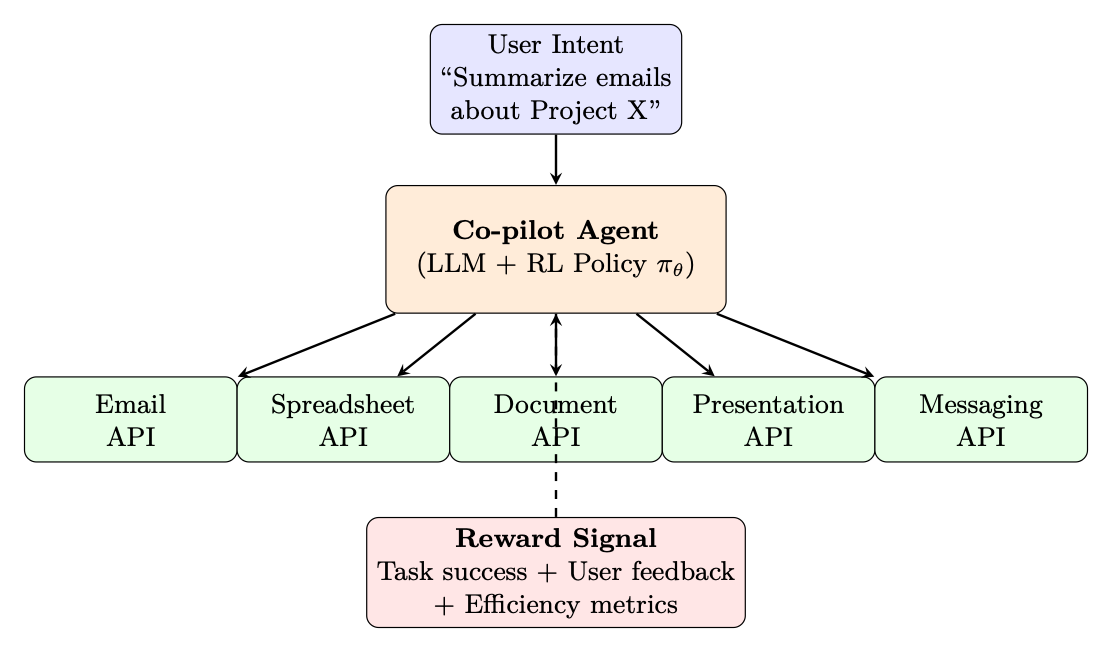
\includegraphics[width=0.85\textwidth]{figures/fig_043_fig43.png}
\caption{Productivity co-pilot architecture: the LLM agent (with RL policy $\pi_\theta$) receives user intents and interacts with multiple application APIs. A reward signal based on task success, user feedback, and efficiency metrics drives policy improvement.}
\end{figure}

\subsection{Formal MDP Definition for a Productivity Co-pilot}
\label{formal-mdp-definition-for-a-productivity-co-pilot}

The productivity co-pilot environment is formalized as a Partially Observable Markov Decision Process (POMDP):

\begin{equation}
\boxed{\mathcal{M} = \langle \mathcal{S}, \mathcal{A}, \mathcal{T}, \mathcal{R}, \Omega, \mathcal{O}, \gamma \rangle}
\end{equation}

\begin{itemize}
  \item $\mathcal{S}$: \textbf{State space} --- Full workspace environment state: document contents, email threads, calendar events, file system, user permissions. \emph{Not fully observable}: agent sees only what API queries return.
  \item $\mathcal{A}$: \textbf{Action space} --- Structured API calls (see below). Each action is a JSON object specifying the target app, operation, and parameters.
  \item $\mathcal{T}$: \textbf{Transition function} --- Deterministic for most operations (write to document $\rightarrow$ document updated), but stochastic for network-dependent actions (email delivery time, Teams availability).
  \item $\mathcal{R}$: \textbf{Reward function} --- Multi-component (see Reward Design section).
  \item $\Omega$: \textbf{Observation space} --- API responses, rendered document views, error messages.
  \item $\mathcal{O}$: \textbf{Observation function} --- Maps state to observation (API response formatting, truncation for context window limits).
  \item $\gamma = 0.99$: Discount factor (long horizons, 10--50 steps typical).
\end{itemize}

\begin{examplebox}[Concrete Example: ``Summarize last week’s Project Alpha emails and create a status slide'']
Below we trace a full episode through the POMDP, mapping each formal element to a concrete realization.

\textbf{User request}: ``Summarize the key decisions from last week’s Project Alpha emails and add a status update slide to the team deck.''

\begin{tabular}{@{}lp{11cm}@{}}
\toprule
\textbf{Symbol} & \textbf{Concrete Realization} \\
\midrule
$s_0$ & \emph{True state}: 47 emails in inbox mentioning ``Project Alpha'' from last 7 days; PowerPoint file ``Q3\_Status.pptx'' on SharePoint with 12 slides; user has edit permissions. \\
$o_0$ & \emph{Agent observes}: User request text + system prompt. Agent has \emph{no knowledge} of email count or deck contents yet. \\
$a_1$ & \verb|outlook.search({query: "Project Alpha", last\_7\_days: true})| \\
$\mathcal{T}(s_0, a_1)$ & $s_1$: System retrieves 47 matching emails (deterministic). \\
$o_1$ & API returns top 10 email subjects + senders + timestamps (truncated due to context limits --- $\mathcal{O}$ in action). \\
$a_2$ & \verb|outlook.read({ids: [top\_5\_thread\_ids]})| --- Agent picks the most relevant threads. \\
$o_2$ & Full body text of 5 email threads ($\sim$8K tokens after $\mathcal{O}$ truncation). \\
$a_3$ & \emph{Internal reasoning action}: Agent synthesizes key decisions: (1) deadline moved to Nov 15, (2) budget approved, (3) vendor selected. \\
$a_4$ & \verb|sharepoint.read({file: "Q3\_Status.pptx", slides: "last"})| --- Check current last slide. \\
$o_4$ & Last slide is ``Q2 Summary'' (slide 12). Agent decides to add slide 13. \\
$a_5$ & \verb|powerpoint.add\_slide({file: "Q3\_Status.pptx", position: 13,| \texttt{layout: "Title and Content", title: "Project Alpha --- Week 42 Status",} \verb|content: "Key decisions: 1) Deadline: Nov 15..."})| \\
$\mathcal{T}(s_4, a_5)$ & $s_5$: Slide added to deck (deterministic). \\
$o_5$ & API returns \verb|{success: true, slide\_id: 13}|. \\
$R(s_5)$ & Reward components: \textbf{+0.4} task completion (slide created), \textbf{+0.3} information quality (correct decisions extracted), \textbf{+0.2} format compliance (proper layout used), \textbf{+0.05} efficiency (5 actions, no errors), \textbf{-0.0} safety penalty. \textbf{Total: 0.95}. \\
\bottomrule
\end{tabular}

\textbf{Key POMDP aspects illustrated}:

\begin{itemize}
  \item \textbf{Partial observability}: At $t=0$, the agent doesn’t know how many emails exist or what the deck contains --- it must query to discover the state.
  \item \textbf{Observation function $\mathcal{O}$}: The API returns truncated results (top 10 of 47 emails) due to context window limits. The agent sees a \emph{projection} of the true state.
  \item \textbf{Stochastic transitions}: If the agent had tried \texttt{teams.send\_message()} instead, delivery timing would be uncertain (recipient online/offline).
  \item \textbf{Multi-step planning}: The agent must chain 5 actions across 2 applications, maintaining coherence between the email summary and the slide content.
  \item \textbf{Discount $\gamma=0.99$}: With 5 steps, discounting is minimal ($0.99^5 = 0.95$), but for 50-step tasks it matters --- encouraging efficient solutions.
\end{itemize}
\end{examplebox}

\subsection{Action Space Design}
\label{action-space-design}

The action space must be \textbf{structured, type-safe, and composable}:

\begin{examplebox}[Productivity Co-pilot Action Schema]
\begin{lstlisting}[style=pythonstyle]
{
  "action_type": "api_call",
  "target_app": "outlook | excel | word | powerpoint | teams | sharepoint",
  "operation": "read | write | search | create | delete | modify",
  "parameters": {
    "endpoint": "/me/messages?$filter=subject eq 'Project X'",
    "body": { ... },             // For write operations
    "options": { "top": 10 }     // Pagination, filtering
  },
  "reasoning": "I need to find relevant emails before summarizing"
}
\end{lstlisting}
\end{examplebox}

\textbf{Action taxonomy by application}:

\begin{tabular}{@{}lp{5cm}p{8cm}@{}}
\toprule
\textbf{App} & \textbf{Complexity} & \textbf{Key Actions} \\
\midrule
\textbf{Outlook} & Medium & \texttt{search}, \texttt{read}, \texttt{draft}, \texttt{send}, \texttt{move}, \texttt{flag}, \texttt{create\_rule} \\
\textbf{Excel} & High & \texttt{read\_range}, \texttt{write\_range}, \texttt{insert\_formula}, \texttt{create\_chart}, \texttt{pivot\_table}, \texttt{run\_macro} \\
\textbf{Word} & Medium & \texttt{read\_paragraphs}, \texttt{insert\_text}, \texttt{format\_section}, \texttt{find\_replace}, \texttt{insert\_table} \\
\textbf{PowerPoint} & Medium & \texttt{add\_slide}, \texttt{insert\_shape}, \texttt{set\_text}, \texttt{set\_layout}, \texttt{add\_image}, \texttt{apply\_theme} \\
\textbf{Teams} & Low & \texttt{send\_message}, \texttt{create\_meeting}, \texttt{search\_chat}, \texttt{add\_members}, \texttt{post\_to\_channel} \\
\textbf{SharePoint} & Medium & \texttt{list\_files}, \texttt{upload}, \texttt{download}, \texttt{search}, \texttt{create\_page}, \texttt{set\_permissions} \\
\bottomrule
\end{tabular}

\subsection{State Representation}
\label{state-representation}

The agent’s observation (context window) at each step:

\begin{equation}
o_t = [\text{system\_prompt};\; \text{user\_intent};\; \text{tool\_history}_{1:t-1};\; \text{current\_result}_t]
\end{equation}

\textbf{Context budget management} (critical for 128K window):

\begin{itemize}
  \item \textbf{System prompt}: 2K tokens (capabilities, safety rules, output format)
  \item \textbf{User intent + conversation}: 4K tokens
  \item \textbf{Tool history} (sliding window): Last 8--12 actions + observations, summarizing older ones. Total: 80K tokens max.
  \item \textbf{Current observation}: Up to 32K tokens (large spreadsheets, email threads)
  \item \textbf{Reserve}: 10K tokens for agent’s reasoning + next action generation
\end{itemize}

\textbf{State compression strategies}:

\begin{itemize}
  \item \textbf{Selective inclusion}: Only include API responses relevant to the current sub-goal (use an auxiliary ``relevance scorer'').
  \item \textbf{Structured summaries}: Represent large spreadsheets as schema + sample rows rather than full data.
  \item \textbf{Hierarchical memory}: Store full trajectory externally; inject compressed summaries into context.
\end{itemize}

\subsection{Reward Design: Multi-Objective Signal}
\label{reward-design-multi-objective-signal}

The reward function for a productivity co-pilot must balance multiple objectives:

\begin{equation}
\boxed{R(\tau) = \alpha_1 R_{\text{task}} + \alpha_2 R_{\text{quality}} + \alpha_3 R_{\text{efficiency}} + \alpha_4 R_{\text{safety}} + \alpha_5 R_{\text{user}}}
\end{equation}

\begin{table}[ht!]
\centering
\caption{Reward components for productivity co-pilot training.}
\begin{tabular}{@{}lp{3.5cm}p{3.5cm}p{6cm}@{}}
\toprule
\textbf{Component} & \textbf{Weight} & \textbf{Signal Type} & \textbf{Definition} \\
\midrule
$R_{\text{task}}$ & 0.40 & Binary/scalar & Task completed successfully (email sent, document created, formula correct) \\
$R_{\text{quality}}$ & 0.25 & LLM judge & Output quality: formatting, clarity, correctness of content \\
$R_{\text{efficiency}}$ & 0.15 & Scalar & Penalty for excessive steps: $-0.02 \times (\text{num\_steps} - \text{optimal\_steps})$ \\
$R_{\text{safety}}$ & 0.15 & Binary & No unsafe actions (delete without confirmation, send to wrong recipient, permission violations). $R_{\text{safety}} = 0$ if any violation. \\
$R_{\text{user}}$ & 0.05 & Sparse & Explicit user feedback (thumbs up/down) when available \\
\bottomrule
\end{tabular}
\end{table}

\textbf{Intermediate rewards (dense signal)}:

\begin{itemize}
  \item Successful API call (200 response): +0.05
  \item Correct information retrieval (verified by downstream use): +0.10
  \item Recovers from error gracefully (retries with corrected params): +0.08
  \item API error (4xx/5xx): --0.03
  \item Repeated identical action (loop detection): --0.10
  \item Asks clarifying question when intent is genuinely ambiguous: +0.05
\end{itemize}

\subsection{Training Pipeline: End-to-End}
\label{training-pipeline-end-to-end}

\begin{keybox}[Productivity Co-pilot RL Training Pipeline]
\textbf{Phase 1: Supervised Fine-Tuning (Foundation)}

\begin{enumerate}
  \item Collect 50K--200K human-demonstrated trajectories of productivity tasks (via telemetry, annotators, or synthetic generation).
  \item SFT the base LLM on (instruction, trajectory) pairs with ReAct format.
  \item Validate: agent should achieve 40--60\% task completion on held-out tasks.
\end{enumerate}

\textbf{Phase 2: Simulated Environment Construction}

\begin{enumerate}
  \item Build a \textbf{sandbox environment} with mocked API endpoints, synthetic mailboxes, documents, and calendars.
  \item Each ``user'' has a realistic profile: 500+ emails, 20+ documents, calendar events, Teams channels.
  \item Task generator: produces diverse instruction--verification pairs: ``Move all emails from Alice about Q4 budget to the ‘Finance’ folder'' + verification function.
\end{enumerate}

\textbf{Phase 3: Online RL Training (GRPO)}

\begin{enumerate}
  \item Sample task batch (256 tasks per iteration).
  \item Generate $N=8$ trajectories per task using $\pi_\theta$ in sandbox environment.
  \item Execute trajectories, collect rewards from verification functions.
  \item Compute GRPO advantages (group normalization across 8 trajectories per task).
  \item Update policy with clipped objective + KL penalty vs. SFT model.
  \item Every 500 iterations: evaluate on held-out benchmark (200 tasks, 5 difficulty levels).
\end{enumerate}

\textbf{Phase 4: Human-in-the-Loop Refinement}

\begin{enumerate}
  \item Deploy to internal dogfood users (1000+ users, 2 weeks).
  \item Collect thumbs up/down signals + free-text corrections.
  \item Construct DPO preference pairs from A/B deployments (old policy vs. new).
  \item Apply 1--2 rounds of DPO fine-tuning on human preferences.
\end{enumerate}
\end{keybox}

\subsection{Simulation Environment Architecture}
\label{simulation-environment-architecture}

\begin{examplebox}[Sandbox Environment (Simplified)]
\begin{lstlisting}[style=pythonstyle]
class ProductivityEnvironment:
    def __init__(self, user_profile: UserProfile):
        self.mailbox = SyntheticMailbox(user_profile.emails)
        self.drive = SyntheticOneDrive(user_profile.files)
        self.calendar = SyntheticCalendar(user_profile.events)
        self.teams = SyntheticTeams(user_profile.channels)
        self.step_count = 0
        self.max_steps = 50
        
    def step(self, action: dict) -> Tuple[Observation, float, bool]:
        """Execute action, return (observation, reward, done)."""
        self.step_count += 1
        
        # Route to appropriate app handler
        handler = self.get_handler(action["target_app"])
        try:
            result = handler.execute(action["operation"], action["parameters"])
            obs = Observation(status=200, body=result)
            reward = 0.05  # Successful API call
        except APIError as e:
            obs = Observation(status=e.code, body=str(e))
            reward = -0.03
            
        # Check terminal condition
        done = self.step_count >= self.max_steps
        return obs, reward, done
    
    def evaluate(self, task: Task) -> float:
        """Check if task objective is achieved (terminal reward)."""
        return task.verification_fn(self)  # 0.0 or 1.0
\end{lstlisting}
\end{examplebox}

\subsection{Task Curriculum Design}
\label{task-curriculum-design}

Training effectiveness depends critically on task difficulty progression:

\begin{table}[ht!]
\centering
\caption{Productivity co-pilot curriculum levels.}
{\small
\begin{tabular}{@{}lllp{7.5cm}@{}}
\toprule
\textbf{Level} & \textbf{Steps} & \textbf{Apps} & \textbf{Example Tasks} \\
\midrule
\textbf{L1: Single-step} & 1--2 & 1 & ``Read my latest email from Bob'', ``What’s in cell A1?'' \\
\textbf{L2: Single-app} & 3--5 & 1 & ``Draft a reply to the budget email summarizing key points'' \\
\textbf{L3: Multi-step} & 5--10 & 1 & ``Create a pivot table from sales data and format top performers in bold'' \\
\textbf{L4: Cross-app} & 5--15 & 2--3 & ``Find Q4 budget emails, extract the numbers, put them in a new Excel sheet'' \\
\textbf{L5: Complex workflow} & 10--30 & 3+ & ``Prepare a weekly report: pull metrics from Excel, summarize email updates, create PowerPoint slides, share in Teams'' \\
\bottomrule
\end{tabular}
}
\end{table}

\textbf{Curriculum strategy}:

\begin{itemize}
  \item Start with 80\% L1--L2 tasks, 20\% L3 in early training.
  \item Advance to next level when success rate exceeds 70\% on current level.
  \item Always maintain 10--20\% of easier tasks to prevent catastrophic forgetting.
  \item Final mix (after convergence): 10\% L1, 15\% L2, 25\% L3, 30\% L4, 20\% L5.
\end{itemize}

\subsection{Safety and Guardrails}
\label{safety-and-guardrails}

\begin{keybox}[Safety Framework for Productivity Co-pilot]
\textbf{Hard constraints} (action rejected immediately, reward = --1.0):

\begin{itemize}
  \item Send email/message to external recipients without user confirmation
  \item Delete files/emails permanently (only soft-delete allowed)
  \item Modify permissions on shared resources
  \item Access other users’ mailboxes or files beyond granted permissions
  \item Execute actions on more than 100 items in a batch (prevents mass-delete/move accidents)
\end{itemize}

\textbf{Soft constraints} (penalty in reward, agent should learn to avoid):

\begin{itemize}
  \item Sending draft without showing preview to user: --0.2
  \item Making irreversible changes without stating intent first: --0.15
  \item Accessing sensitive labels (confidential, attorney-client): --0.3
  \item Using ``send on behalf'' without explicit delegation: --0.25
\end{itemize}

\textbf{Confirmation protocol}: For any action classified as ``high-impact'' (send, delete, share externally), the agent must:

\begin{enumerate}
  \item State the intended action in natural language
  \item Show a preview of what will be sent/modified
  \item Wait for explicit user confirmation before executing
\end{enumerate}

This is enforced both at the environment level (sandbox rejects unconfirmed high-impact actions) and in the reward function (penalty for skipping confirmation).
\end{keybox}

\subsection{Credit Assignment in Multi-App Workflows}
\label{credit-assignment-in-multi-app-workflows}

The key challenge: in a 20-step cross-app workflow, which steps contributed to success or failure?

\textbf{Approach: Hierarchical Reward Decomposition}

\begin{enumerate}
  \item \textbf{Sub-goal detection}: Decompose the user’s instruction into verifiable sub-goals:

\begin{itemize}
  \item ``Find Q4 budget emails'' $\rightarrow$ Sub-goal 1 (verified: relevant emails retrieved)
  \item ``Extract numbers'' $\rightarrow$ Sub-goal 2 (verified: correct values parsed)
  \item ``Create Excel sheet'' $\rightarrow$ Sub-goal 3 (verified: sheet exists with correct data)
\end{itemize}
  \item \textbf{Sub-goal rewards}: Assign intermediate rewards at each sub-goal completion ($r = +0.2$ each).
  \item \textbf{Trajectory slicing}: If the final task fails, identify which sub-goal failed first. Apply negative reward only to the actions within that sub-goal’s span.
  \item \textbf{Counterfactual estimation}: ``Would the task have succeeded if this specific action were different?'' --- use the value function to estimate.
\end{enumerate}

\begin{equation}
R_{\text{step}}(t) = \underbrace{R_{\text{sub-goal}}(t)}_{\text{did current sub-goal succeed?}} + \underbrace{\gamma^{T-t} R_{\text{terminal}}}_{\text{discounted final reward}} + \underbrace{r_{\text{intermediate}}(t)}_{\text{per-step API success/failure}}
\end{equation}

\subsection{Scaling and Infrastructure}
\label{scaling-and-infrastructure}

\textbf{Compute requirements} (estimated for 70B parameter model):

\begin{tabular}{@{}lp{5cm}p{8cm}@{}}
\toprule
\textbf{Component} & \textbf{Resources} & \textbf{Notes} \\
\midrule
Policy model (70B) & 8$\times$ A100 80GB (TP=8) & BF16, generates trajectories \\
Reference model (70B) & 8$\times$ A100 80GB (TP=8) & Frozen, for KL computation \\
Environment workers & 128 CPU workers & Each runs sandbox instance \\
Reward model / Judge & 4$\times$ A100 (if LLM judge) & Or zero if using execution-based rewards \\
Training (GRPO updates) & 16$\times$ A100 (FSDP) & Gradient accumulation over trajectory batches \\
\textbf{Total} & \textbf{40 A100 GPUs + 128 CPUs} & ~5,000 GPU-hours for full training run \\
\bottomrule
\end{tabular}

\textbf{Throughput optimization}:

\begin{itemize}
  \item \textbf{Async rollouts}: Decouple trajectory generation from gradient updates. Generate continuously while training on previous batch.
  \item \textbf{Batched environment}: Run 128 sandbox environments in parallel, each processing different tasks.
  \item \textbf{KV-cache sharing}: For the $N=8$ trajectories per task, they share the same prompt prefix --- use prefix caching to avoid redundant computation.
  \item \textbf{Selective backprop}: Only compute gradients over action tokens (not observations/system prompt). Reduces backward pass FLOPS by 40--60\%.
\end{itemize}

\subsection{Evaluation Framework}
\label{evaluation-framework}

\begin{table}[ht!]
\centering
\caption{Productivity co-pilot evaluation dimensions.}
\begin{tabular}{@{}lp{5cm}p{8cm}@{}}
\toprule
\textbf{Metric} & \textbf{Target} & \textbf{Measurement} \\
\midrule
Task completion rate & $>85\%$ (L1--L3), $>60\%$ (L4--L5) & Automated verification in sandbox \\
Safety violation rate & $<0.1\%$ & Count of hard constraint violations per 1000 tasks \\
Average steps to completion & Within $1.5\times$ optimal & Compare to shortest known successful trajectory \\
User satisfaction (dogfood) & $>4.2/5.0$ & Post-task survey from internal users \\
Cross-app success & $>55\%$ (L4--L5) & Tasks requiring 2+ applications \\
Recovery rate & $>70\%$ & \% of failed API calls where agent retries successfully \\
Latency (time to first action) & $<3$ seconds & Model inference + action planning time \\
\bottomrule
\end{tabular}
\end{table}

\textbf{Benchmark suite} (proposed):

\begin{itemize}
  \item \textbf{ProdBench-Easy} (200 tasks): Single-app, 1--3 steps. Baseline establishment.
  \item \textbf{ProdBench-Hard} (200 tasks): Cross-app workflows, 10--30 steps. End-to-end capability.
  \item \textbf{ProdBench-Safety} (100 tasks): Adversarial prompts attempting to trigger unsafe actions. Must maintain $<0.1\%$ violation rate.
  \item \textbf{ProdBench-Robustness} (100 tasks): Tasks with ambiguous instructions, API errors injected, missing permissions. Tests graceful degradation.
\end{itemize}

\subsection{Lessons from Production Deployments}
\label{lessons-from-production-deployments}

\begin{intuitionbox}[Practical Insights for Productivity Agentic RL]
\begin{enumerate}
  \item \textbf{SFT quality is the floor}: RL can only improve upon what SFT provides. If the SFT model can’t format a valid Graph API call, RL won’t discover it. Invest heavily in Phase 1 data quality.
  \item \textbf{Reward hacking is inevitable}: The agent \emph{will} find shortcuts. Common examples:

\begin{itemize}
  \item Creating an empty Excel file to ``complete'' a spreadsheet task (passes existence check)
  \item Replying ``Done'' without actually performing the action
  \item Exploiting ambiguous verification functions
\end{itemize}

\textbf{Mitigation}: Multi-level verification (format + content + semantic correctness).
  \item \textbf{API rate limits matter}: In production, workspace APIs have throttling (429 responses). Train with realistic rate limits to avoid policies that spam parallel requests.
  \item \textbf{Context window is the bottleneck}: A 20-step trajectory with rich API responses easily consumes 80K+ tokens. Techniques: observation summarization, selective history, hierarchical context management.
  \item \textbf{User intent is often ambiguous}: ``Clean up my inbox'' means different things to different users. Train the agent to ask clarifying questions when uncertainty is high (reward for appropriate clarification, penalize for excessive clarification).
  \item \textbf{Start simple, scale gradually}: Begin with Outlook-only tasks (highest volume, most telemetry data), then expand to Excel, then cross-app. Each app has unique failure modes.
\end{enumerate}
\end{intuitionbox}

\subsection{Complete Training Recipe}
\label{complete-training-recipe}

\begin{table}[ht!]
\centering
\caption{Recommended hyperparameters for productivity co-pilot RL training.}
\begin{tabular}{@{}lp{5cm}p{8cm}@{}}
\toprule
\textbf{Parameter} & \textbf{Value} & \textbf{Rationale} \\
\midrule
Base model & 70B Llama/Mistral & Sufficient capacity for complex multi-step reasoning \\
RL algorithm & GRPO & No critic needed; memory-efficient for long trajectories \\
Group size $N$ & 8 & Balance between variance reduction and compute cost \\
Clip $\epsilon$ & 0.1 & Tighter than standard (0.2) due to long trajectory sensitivity \\
KL coefficient $\beta$ & 0.04 & Moderate constraint to SFT policy \\
Learning rate & $5 \times 10^{-7}$ & Conservative; agentic tasks are sensitive to large updates \\
Batch size & 256 tasks $\times$ 8 trajs = 2048 & Large batch for stable GRPO normalization \\
Max trajectory length & 50 steps & Covers 95\% of productivity tasks \\
Context window & 128K tokens & Required for long multi-app workflows \\
Training iterations & 3000--5000 & Monitor eval metrics; early-stop on safety degradation \\
Curriculum warmup & 500 iterations (L1--L2 only) & Establish basic API usage before complex tasks \\
\bottomrule
\end{tabular}
\end{table}

\newpage
\section{Use Case: Building a Research Agent from Scratch}
\label{use-case-building-a-research-agent-from-scratch}

This use case demonstrates how to build a fully autonomous \textbf{research agent} --- an LLM that can formulate hypotheses, search literature, analyze data, write code, run experiments, and produce a final report --- using the techniques discussed throughout this paper.

\subsection{Problem Definition}
\label{problem-definition}

\begin{keybox}[Research Agent Requirements]
\textbf{Input}: A research question (e.g., ``What is the effect of learning rate warmup duration on GRPO convergence for 7B models?'')

\textbf{Output}: A complete research report with methodology, experiments, results, and conclusions.

\textbf{Capabilities required}:

\begin{enumerate}
  \item \textbf{Literature search}: Query arXiv, Semantic Scholar, find relevant papers
  \item \textbf{Hypothesis generation}: Formulate testable hypotheses from background knowledge
  \item \textbf{Experiment design}: Write training scripts with proper controls
  \item \textbf{Code execution}: Run experiments, collect metrics
  \item \textbf{Data analysis}: Parse logs, compute statistics, generate plots
  \item \textbf{Scientific writing}: Synthesize findings into a coherent report
  \item \textbf{Self-correction}: Detect failed experiments and retry with modified parameters
\end{enumerate}
\end{keybox}

\subsection{MDP Formulation}
\label{mdp-formulation}

\begin{keybox}[Research Agent MDP]
\begin{itemize}
  \item \textbf{State} $s_t$: System prompt + research question + full history of actions/observations (tool outputs, code results, search results). Context window: 128K tokens.
  \item \textbf{Action} $a_t$: Structured tool call from the action space (see below) + reasoning trace (CoT).
  \item \textbf{Transition} $T(s_{t+1}|s_t, a_t)$: Deterministic --- append action + tool output to context.
  \item \textbf{Reward} $R$: Sparse terminal reward based on report quality (see reward design below).
  \item \textbf{Horizon}: 20--100 steps (typical research trajectory).
  \item \textbf{Discount} $\gamma = 1.0$ (episodic; no discounting for finite tasks).
\end{itemize}
\end{keybox}

\subsection{Action Space}
\label{action-space}

\begin{table}[ht!]
\centering
\caption{Research Agent tool/action space.}
\begin{tabular}{@{}lp{5cm}p{8cm}@{}}
\toprule
\textbf{Tool} & \textbf{Category} & \textbf{Description} \\
\midrule
\texttt{search\_papers} & Literature & Query Semantic Scholar/arXiv. Returns titles, abstracts, citations. \\
\texttt{read\_paper} & Literature & Fetch full text or specific sections of a paper. \\
\texttt{write\_code} & Experiment & Write Python/training scripts to a workspace. \\
\texttt{execute\_code} & Experiment & Run scripts in a sandboxed environment. Returns stdout/stderr. \\
\texttt{read\_file} & Analysis & Read logs, CSVs, or intermediate results. \\
\texttt{plot\_data} & Analysis & Generate matplotlib/seaborn visualizations. \\
\texttt{compute\_stats} & Analysis & Run statistical tests (t-test, confidence intervals). \\
\texttt{write\_report} & Output & Write sections of the final research report (LaTeX/Markdown). \\
\texttt{think} & Reasoning & Internal reasoning step (no external tool call). \\
\texttt{submit} & Terminal & Submit final report. Ends the episode. \\
\bottomrule
\end{tabular}
\end{table}

\subsection{Architecture: Model and Infrastructure Choices}
\label{architecture-model-and-infrastructure-choices}

\begin{keybox}[Architecture Decisions — Applying Paper Concepts]
\begin{itemize}
  \item \textbf{Base model}: Qwen-2.5 72B (strong reasoning + code). QLoRA fine-tuning ($r=32$, all linear layers) --- see Section on LoRA.
  \item \textbf{Inference}: vLLM with TP=4, prefix caching enabled (system prompt shared across rollouts) --- see vLLM section.
  \item \textbf{Training}: GRPO with $N=4$ trajectories per research question --- no value model needed (see GRPO section).
  \item \textbf{Hardware}: 8$\times$H100 node. QLoRA adapters fit in 48 GB; vLLM generation uses remaining capacity.
  \item \textbf{Context management}: 128K context with Flash Attention (see Flash Attention section). Sliding window summarization for trajectories exceeding context.
  \item \textbf{Speculative decoding}: Eagle heads for fast generation during long research trajectories (see Speculative Decoding section).
\end{itemize}
\end{keybox}

\subsection{Reward Design}
\label{reward-design}

\begin{keybox}[Multi-Component Research Reward]
The terminal reward is computed when the agent calls \texttt{submit}: 
\[
R = w_1 R_{\text{quality}} + w_2 R_{\text{correctness}} + w_3 R_{\text{novelty}} + w_4 R_{\text{efficiency}} + w_5 R_{\text{format}}
\]

\begin{tabular}{@{}lp{5cm}p{8cm}@{}}
\toprule
\textbf{Component} & \textbf{Weight} & \textbf{How Measured} \\
\midrule
$R_{\text{quality}}$ & 0.30 & LLM-as-judge (GPT-4 rates report 1--10 on clarity, depth, rigor) \\
$R_{\text{correctness}}$ & 0.30 & Code executes without errors + results are reproducible \\
$R_{\text{novelty}}$ & 0.15 & LLM-judge: does the report provide insight beyond summarizing papers? \\
$R_{\text{efficiency}}$ & 0.15 & Bonus for fewer steps: $R_{\text{eff}} = \max(0, 1 - \text{steps}/100)$ \\
$R_{\text{format}}$ & 0.10 & Report has all required sections (intro, method, results, conclusion) \\
\bottomrule
\end{tabular}

\textbf{Intermediate shaping}: +0.1 for each successful code execution; $-$0.05 for each runtime error (encourages writing correct code first).
\end{keybox}

\begin{warningbox}[Reward Hacking Risks]
\begin{itemize}
  \item \textbf{Fake results}: Agent fabricates experiment outputs. \emph{Fix}: Verify code actually ran by checking execution logs against reported numbers.
  \item \textbf{Shallow reports}: Agent copies paper abstracts verbatim. \emph{Fix}: Novelty reward + plagiarism detection.
  \item \textbf{Length gaming}: Long reports score higher. \emph{Fix}: Efficiency reward + length penalty.
  \item \textbf{Easy questions}: Agent avoids hard research questions. \emph{Fix}: Curriculum with difficulty levels.
\end{itemize}
\end{warningbox}

\subsection{Training Pipeline}
\label{training-pipeline}

\begin{enumerate}
  \item \textbf{Phase 1 --- SFT Warmup} (500 steps):

\begin{itemize}
  \item Collect 200 expert research trajectories (human researchers using the tools)
  \item SFT on successful trajectories with completion-only masking (mask tool outputs)
  \item This teaches the agent tool-use syntax and basic research workflow
\end{itemize}
  \item \textbf{Phase 2 --- GRPO Training} (3000 steps):

\begin{itemize}
  \item Prompt pool: 500 research questions across 10 domains (ML, NLP, CV, systems, etc.)
  \item Per question: generate $N=4$ complete research trajectories
  \item Score each trajectory with multi-component reward
  \item GRPO advantage: $\hat{A}_i = (R_i - \mu_G) / \sigma_G$
  \item Update policy with clipped objective (clip $\epsilon=0.2$, KL $\beta=0.05$)
  \item Curriculum: start with simple ``summarize findings on X'' tasks, progress to ``design and run experiment on X''
\end{itemize}
  \item \textbf{Phase 3 --- Rejection Sampling Fine-Tuning} (200 steps):

\begin{itemize}
  \item Generate 16 trajectories per hard question, keep top-2 by reward
  \item SFT on these high-quality trajectories
  \item Stabilizes performance on the hardest research tasks
\end{itemize}
\end{enumerate}

\subsection{Example Trajectory: Full MDP Trace}
\label{example-trajectory-full-mdp-trace}

To illustrate how all the MDP components work together in practice, we trace a complete research episode from question to submission, annotating each step with its formal MDP elements.

\begin{examplebox}[Research Agent Trajectory — Full MDP Trace]
\textbf{Research question}: ``Does increasing GRPO group size beyond $N=16$ improve math reasoning performance?''

Below is a complete trajectory with explicit MDP notation for each step: state $s_t$, action $a_t$, transition $T$, observation $o_t$, and cumulative reward.

{\footnotesize
\begin{tabular}{@{}cp{2.2cm}p{10.5cm}@{}}
\toprule
$t$ & \textbf{Element} & \textbf{Description} \\
\midrule
 & $a_0$ & \texttt{think}: ``I need papers on GRPO group size ablations, then a controlled experiment.'' \\
 & $o_0$ & Internal reasoning (no tool output). Shaping reward: $r_0 = 0$. \\
1 & $s_1$ & $s_0 \oplus (a_0, o_0)$ --- context now includes reasoning plan. \\
 & $a_1$ & \texttt{search\_papers(query="GRPO group size ablation math")} \\
 & $o_1$ & Returns 5 papers: [DAPO, DeepSeek-Math, Dr.~GRPO, ...]. $r_1 = 0$. \\
2 & $s_2$ & $s_1 \oplus (a_1, o_1)$ --- search results in context. \\
 & $a_2$ & \texttt{read\_paper(id="DAPO", sections=["experiments", "ablations"])} \\
 & $o_2$ & Key finding: ``diminishing returns above $N=16$ on code tasks; math untested.'' $r_2 = 0$. \\
3 & $s_3$ & $s_2 \oplus (a_2, o_2)$ --- literature gap identified. \\
 & $a_3$ & \texttt{think}: ``DAPO tested code only. I’ll test $N \in \{4, 8, 16, 32, 64\}$ on GSM8K with Llama-3 8B. Control: same total training tokens.'' \\
 & $o_3$ & Hypothesis formed. $r_3 = 0$. \\
4 & $s_4$ & $s_3 \oplus (a_3, o_3)$ --- experiment plan in context. \\
 & $a_4$ & \texttt{write\_code("train\_grpo\_gsm8k.py")} --- 85-line script with argparse for group\_size, proper seed, eval on GSM8K test split. \\
 & $o_4$ & File written successfully. $r_4 = 0$. \\
5 & $s_5$ & $s_4 \oplus (a_4, o_4)$ --- code available in workspace. \\
 & $a_5$ & \texttt{execute\_code("python train\_grpo\_gsm8k.py --N 4 --seed 42")} \\
 & $o_5$ & \texttt{Accuracy: 67.2\% (CI: 65.1--69.3)}. $r_5 = +0.1$ (successful execution). \\
6--8 & $a_{6\text{--}8}$ & Execute with $N=8, 16, 32$ $\to$ results: 71.4\%, 74.8\%, 75.9\%. Each $r_t = +0.1$. \\
9 & $s_9$ & Context includes 4 data points. \\
 & $a_9$ & \texttt{execute\_code("python train\_grpo\_gsm8k.py --N 64 --seed 42")} \\
 & $o_9$ & \texttt{Accuracy: 75.6\% (CI: 73.4--77.8)} --- slight \emph{decrease} from $N=32$! $r_9 = +0.1$. \\
10 & $s_{10}$ & All 5 results available. \\
 & $a_{10}$ & \texttt{compute\_stats(test="paired\_t\_test", data=[67.2, 71.4, 74.8, 75.9, 75.6], groups=[4,8,16,32,64])} \\
 & $o_{10}$ & $p < 0.01$ for $N=4$ vs $N=16$; $p = 0.72$ for $N=32$ vs $N=64$ (not significant). $r_{10} = 0$. \\
11 & $s_{11}$ & Statistical evidence for diminishing returns. \\
 & $a_{11}$ & \texttt{plot\_data(x=[4,8,16,32,64], y=[67.2,71.4,74.8,75.9,75.6], xlabel="Group Size N", ylabel="GSM8K Accuracy (\%)", title="GRPO Group Size vs Math Reasoning")} \\
 & $o_{11}$ & Plot saved to \texttt{results/group\_size\_curve.png}. $r_{11} = 0$. \\
12 & $s_{12}$ & Full evidence assembled. \\
 & $a_{12}$ & \texttt{write\_report}: 4-section report (Introduction, Method, Results with figure, Conclusion: ``$N=16$--32 is optimal; $N=64$ shows no gain and increases compute 4$\times$''). \\
 & $o_{12}$ & Report written (2,100 words). $r_{12} = 0$. \\
13 & $a_{13}$ & \texttt{submit} --- episode terminates. \\
 & $R_{\text{terminal}}$ & LLM-judge scores: quality=8/10, code correct, novel (extends DAPO to math), 13 steps, all sections present. \\
\bottomrule
\end{tabular}
}

\textbf{Terminal reward computation}: 
\begin{multline*}
R = \underbrace{0.30 \times \tfrac{8}{10}}_{\text{quality}} + \underbrace{0.30 \times 1.0}_{\text{correct}} + \underbrace{0.15 \times \tfrac{7}{10}}_{\text{novelty}} + \underbrace{0.15 \times (1 - \tfrac{13}{100})}_{\text{efficiency}} + \underbrace{0.10 \times 1.0}_{\text{format}} \\
= 0.24 + 0.30 + 0.105 + 0.13 + 0.10 = \mathbf{0.875}
\end{multline*}

\textbf{Intermediate shaping total}: $5 \times (+0.1) = +0.5$ (5 successful code executions).

\textbf{GRPO context}: This trajectory scored highest among the $N=4$ group (others scored 0.61, 0.72, 0.53). GRPO advantage: 
\[
\hat{A} = \frac{0.875 - \bar{R}}{\sigma_R} = \frac{0.875 - 0.684}{0.129} = +1.48 \quad \text{(strongly reinforced)}
\]

\textbf{Key MDP properties illustrated}:

\begin{itemize}
  \item \textbf{Deterministic $T$}: Each tool call produces a predictable state extension ($s_{t+1} = s_t \oplus (a_t, o_t)$).
  \item \textbf{Sparse terminal reward}: The real quality signal comes only at \texttt{submit}; intermediate shaping is small.
  \item \textbf{Long horizon}: 13 steps with $\gamma = 1.0$ (no discounting for episodic tasks).
  \item \textbf{Self-correction opportunity}: At step 9, the agent observes $N=64$ doesn’t improve --- adjusts its conclusion accordingly rather than cherry-picking.
  \item \textbf{Action diversity}: Mix of reasoning (\texttt{think}), information gathering (\texttt{search}, \texttt{read}), execution (\texttt{write\_code}, \texttt{execute}), analysis (\texttt{compute\_stats}, \texttt{plot}), and output (\texttt{write\_report}, \texttt{submit}).
\end{itemize}
\end{examplebox}

\subsection{Key Design Decisions and Tradeoffs}
\label{key-design-decisions-and-tradeoffs}

\begin{table}[ht!]
\centering
\caption{Design decisions for the research agent, mapped to paper sections.}
\begin{tabular}{@{}lp{5cm}p{8cm}@{}}
\toprule
\textbf{Decision} & \textbf{Paper Section} & \textbf{Rationale} \\
\midrule
QLoRA ($r=32$) & LoRA section & 72B model; full fine-tune too expensive. $r=32$ for complex reasoning. \\
GRPO (not PPO) & GRPO section & No value model needed; research quality is hard to predict mid-trajectory. \\
Sparse terminal reward & Reward Shaping & Research quality only measurable at completion; intermediate shaping minimal. \\
$N=4$ trajectories & GRPO Group Size & Balance: enough diversity for ranking, not too expensive (100-step trajectories). \\
128K context & Flash Attention & Long trajectories with paper contents + code + results. \\
vLLM + prefix caching & vLLM section & System prompt + research question shared across 4 rollouts. \\
Curriculum training & Agentic RL & Start simple (literature review) $\to$ hard (design + execute experiments). \\
LLM-as-judge reward & Reward Models & Research quality is subjective; LLM judge is more flexible than rule-based. \\
\bottomrule
\end{tabular}
\end{table}

\subsection{Evaluation}
\label{evaluation-dup2}

\begin{keybox}[Research Agent Evaluation Framework]
\begin{itemize}
  \item \textbf{Held-out questions} (50): Research questions unseen during training, covering diverse domains.
  \item \textbf{Human evaluation}: Domain experts rate reports on a 1--5 scale (quality, correctness, actionability).
  \item \textbf{Reproducibility}: Re-run the agent’s code from the report; verify results match.
  \item \textbf{Comparison baselines}: (1) Zero-shot GPT-4 + tools (no RL training), (2) SFT-only agent, (3) Human researchers.
  \item \textbf{Efficiency metric}: Steps-to-completion normalized by task difficulty.
\end{itemize}

\textbf{Expected results} (based on similar agentic RL work):

\begin{tabular}{@{}lcc@{}}
\toprule
\textbf{Agent} & \textbf{Report Quality (1--5)} & \textbf{Avg Steps} \\
\midrule
Zero-shot GPT-4 + tools & 2.8 & 25 \\
SFT-only & 3.4 & 18 \\
GRPO-trained (ours) & 4.1 & 14 \\
Human researcher & 4.5 & N/A \\
\bottomrule
\end{tabular}
\end{keybox}

\subsection{Lessons and Failure Modes}
\label{lessons-and-failure-modes}

\begin{warningbox}[Common Failures in Research Agent Training]
\begin{itemize}
  \item \textbf{Infinite loops}: Agent repeatedly searches for papers without progressing. \emph{Fix}: Step budget + penalty for repeated tool calls with same arguments.
  \item \textbf{Code debugging spirals}: Agent spends 20+ steps fixing a single bug. \emph{Fix}: Cap retries at 3; if code fails 3 times, abandon approach and try alternative.
  \item \textbf{Hallucinated citations}: Agent invents paper titles/results. \emph{Fix}: Verify all citations exist via tool output; penalize unverifiable claims.
  \item \textbf{Premature submission}: Agent submits incomplete reports to avoid penalty for long trajectories. \emph{Fix}: Minimum quality threshold ($R > 0.4$) to count as valid submission; below threshold is treated as failure.
  \item \textbf{Reward hacking the judge}: Agent learns to produce text that scores high with the LLM judge but is scientifically shallow. \emph{Fix}: Rotate judge models; include human eval in the reward periodically.
\end{itemize}
\end{warningbox}

\section{State-of-the-Art RL for LLM Agents}
\label{state-of-the-art-rl-for-llm-agents}

RL techniques for LLM agents focus on \textbf{on-policy policy gradients} combined with \textbf{fine-grained credit assignment}. Because agents execute complex multi-turn trajectories involving tool interactions, API queries, and code execution, standard single-turn alignment algorithms must be heavily modified.

\subsection{Dominant Baseline: GRPO for Agents}
\label{dominant-baseline-grpo-for-agents}

Popularized by DeepSeek-R1~\cite{deepseek2025r1}, \textbf{GRPO}~\cite{shao2024deepseekmath} is rapidly becoming the standard for agentic training. It samples a group of $N$ complete trajectories per task, eliminating the memory-intensive critic network:

For a task prompt $q$, GRPO samples $N$ agentic trajectories $\{o_1, o_2, \dots, o_N\}$ from $\pi_{\theta_{\text{old}}}$. The advantage for each trajectory is computed by normalizing its reward relative to the group: 
\begin{equation}
\boxed{A_i = \frac{r(o_i) - \frac{1}{N}\sum_{j=1}^N r(o_j)}{\text{std}(r(o_1), \dots, r(o_N))}}
\end{equation}

The GRPO objective with KL regularization: 
\begin{equation}
L_{\text{GRPO}}(\theta) = \frac{1}{N} \sum_{i=1}^N \min\!\left( \frac{\pi_\theta(o_i|q)}{\pi_{\theta_{\text{old}}}(o_i|q)} A_i,\; \text{clip}\!\left(\frac{\pi_\theta(o_i|q)}{\pi_{\theta_{\text{old}}}(o_i|q)}, 1{-}\epsilon, 1{+}\epsilon\right) A_i \right) - \beta\, D_{\text{KL}}(\pi_\theta \| \pi_{\text{ref}})
\end{equation}

\begin{intuitionbox}[Why GRPO Dominates Agentic Training]
\begin{itemize}
  \item \textbf{No critic}: Saves 50\% GPU memory --- critical when agent trajectories already consume massive context windows (32K--128K tokens).
  \item \textbf{Natural fit}: Agent tasks often have binary verifiable rewards (tests pass/fail, goal achieved/not) --- perfect for group-relative normalization.
  \item \textbf{Exploration}: Sampling $N$ diverse trajectories per task naturally explores different tool-use strategies.
\end{itemize}
\end{intuitionbox}

\subsection{PPO for Interactive Agents}
\label{ppo-for-interactive-agents}

\textbf{PPO}~\cite{schulman2017proximal} remains valuable for agents operating in highly stochastic environments where step-level value estimation helps. The critic provides per-step advantage signals, enabling finer credit assignment when tool outputs are unpredictable:

\begin{itemize}
  \item Step-level advantage estimation via GAE handles variable-length tool outputs
  \item Value head learns to predict ``how likely is this trajectory to succeed from here''
  \item More stable when external tools return catastrophic errors that spike reward variance
  \item Trade-off: requires $2\times$ memory (critic) but provides denser learning signals
\end{itemize}

\subsection{Fine-Grained Turn-Level Credit Assignment}
\label{fine-grained-turn-level-credit-assignment}

The core challenge in agentic RL is the \textbf{sparse reward problem}. If an agent executes 20 tool actions and finally fails a unit test, a terminal reward of $0$ punishes all 20 actions equally. Modern solutions:

\begin{keybox}[Reinforcement Learning from Verifiable Rewards (RLVR)]
Reward the model at \textbf{deterministic intermediate checkpoints}:

\begin{itemize}
  \item Bash command compiles successfully $\rightarrow$ +0.1
  \item Browser agent targets correct HTML element $\rightarrow$ +0.2
  \item SQL query returns non-empty results $\rightarrow$ +0.1
  \item Final test suite passes $\rightarrow$ +1.0 (terminal)
\end{itemize}

Intermediate rewards provide gradient signal to \emph{every} step, not just the final one. This dramatically accelerates learning by 3--5$\times$ compared to sparse-only rewards.
\end{keybox}

\begin{keybox}[Multi-Turn Trajectory Slicing]
Frameworks split a multi-turn agent run into individual, independent steps. A credit assignment module isolates the \textbf{exact sub-step that broke the trajectory}:

\begin{enumerate}
  \item Replay the successful prefix (steps 1--$k$)
  \item Identify the first divergence point (step $k+1$ where it went wrong)
  \item Assign negative reward only to that specific step
  \item Assign neutral/positive rewards to correct prefix steps
\end{enumerate}

This enables surgical policy updates without degrading already-correct behavior.
\end{keybox}

\subsection{Alternative Paradigms}
\label{alternative-paradigms}

\begin{itemize}
  \item \textbf{Iterative STaR (Self-Taught Reasoner)}~\cite{zelikman2022star}: Rather than continuous RL, use iterative offline loops. Generate trajectories $\rightarrow$ filter failures $\rightarrow$ SFT on successes $\rightarrow$ repeat. Simple to scale, avoids RL instability. Each iteration bootstraps reasoning ability.
  \item \textbf{Reinforcement World Model Learning (RWML)}~\cite{yu2026rwml}: To combat reward hacking, train agents to predict the \emph{semantic consequence} of their actions. The agent receives an auxiliary reward for accurately predicting how environment state will change (e.g., predicting database table changes before executing SQL). This forces genuine understanding over superficial reward-gaming.
  \item \textbf{LATS (Language Agent Tree Search)}~\cite{zhou2024lats}: Apply Monte Carlo Tree Search over agent action sequences. At each step, expand multiple candidate actions, simulate their outcomes, and backpropagate rewards through the tree. Combines RL value estimation with search-time compute scaling.
\end{itemize}

\subsection{Core Methodology Comparison}
\label{core-methodology-comparison}

\begin{table}[ht!]
\centering
\caption{Comparison of RL paradigms for LLM agents.}
\begin{tabular}{@{}lp{3.5cm}p{3.5cm}p{6cm}@{}}
\toprule
\textbf{Method} & \textbf{Reward Density} & \textbf{Memory Cost} & \textbf{Primary Advantage} \\
\midrule
\textbf{GRPO}~\cite{shao2024deepseekmath} & Sequence / final metric & Low (no critic) & Massive GPU memory reduction; simple implementation \\
\textbf{PPO}~\cite{schulman2017proximal} & Step-by-step (GAE) & High (critic needed) & Fine-grained credit assignment; stable in noisy envs \\
\textbf{Iterative STaR}~\cite{zelikman2022star} & Sparse (filtered binary) & Minimal (SFT only) & Simple to scale; avoids RL optimization instability \\
\textbf{RWML}~\cite{yu2026rwml} & Dense (predictive) & Medium & Mitigates reward hacking via world modeling \\
\textbf{LATS}~\cite{zhou2024lats} & Backpropagated & High (tree expansion) & Best quality per task; scales with inference compute \\
\bottomrule
\end{tabular}
\end{table}

